% TODO bibliography?
% TODO 
% acknowledgement screen
% formulas a bit heavy
% some slides heavy, use boxes
% Aspect ratio
\documentclass{beamer}
\usepackage{animate}
\usepackage[english]{babel}
\usepackage[utf8]{inputenc}
\usepackage{algorithm}
\usepackage[noend]{algpseudocode}
\usepackage{graphics}
\usepackage[final]{pdfpages}
\usepackage[font=small, skip=0pt]{caption}
\setbeamertemplate{frametitle continuation}[from second][(contd.)]
\setbeamertemplate{itemize items}{--}
\beamertemplatenavigationsymbolsempty

\title{Proximal Policy Optimization with Dynamic Clipping}
\author{Student: Rishikesh Vaishnav\\Mentor: Sicun Gao}

\begin{document}
\captionsetup{labelformat=empty, font=footnotesize}
\renewcommand{\thealgorithm}{}
\maketitle
\begin{frame}[noframenumbering, allowframebreaks]{Background}
    Reinforcement Learning
    \begin{itemize}
        \item A set of algorithms that seek to replicate behavioral learning.
        \item Basic vocabulary:
        \begin{itemize}
            \item \textbf{Environment}: a general setting with changeable
                parameters in which actions can be performed that affect these
                parameters
            \item \textbf{State} (denoted $s$): a specific configuration (i.e. ``snapshot'')
                of an environment
            \item \textbf{Agent}: an entity that learns to accomplish a task in
                a specific evironment
            \item \textbf{Action} (denoted $a$): a decision made by the agent that is intended
                to affect subsequent states
            \item \textbf{Episode}: a sequence of states and actions in an
                environment
            \item \textbf{Reward} (denoted $r$): a number associated with a state-action pair
        \end{itemize}
        \item Overall goal: train an agent that picks actions such that the sum
            of the rewards over an episode is maximimized.
        \framebreak
        \item Example: cart-pole demo
            \animategraphics[autoplay,loop,width=\linewidth]{25}
                {cartpole_ex/coalesced/cartpole_ex-}{0}{372}
        % NOTE explain how each of the previous terms manifests itself in this
        % example
    \end{itemize}
    \framebreak
    Policy Gradient Methods
    \begin{itemize}
        \item An agent can be provided with a \textbf{policy}, usually denoted
            $\pi$, that completely specifies the probabilty distribution of the
            action that should be taken at any particular state.
        \item $\pi$ is parameterized by some vector $\theta$ and can be any
            function of a state $s_t$.
        % NOTE mention that this is usually done using neural networks, in
        % which context theta is the vector of weights
        \item The task of the agent is to learn $\theta$.
        \begin{align*}
            s \rightarrow NN(\theta) \rightarrow \pi(a)
        \end{align*}
    \end{itemize}
    \framebreak
    Generic Policy Gradient Algorithm
    \begin{algorithm}[H]
        \caption{Generic Policy Gradient}
        \begin{algorithmic}
            \State Initialize $\theta$ arbitrarily
            \While{True}\Comment{loop forever}
                \State $\theta_{old} \gets \theta$
                \State $rollout \gets (s, a, r)$ from multiple
                $\pi_{\theta}$ episodes 
                % NOTE explain what a rollout is and what (s, a, r) are
                \State Set $\theta$ to maximize the loss function $L(rollout,
                \theta, \theta_{old})$
            \EndWhile
        \end{algorithmic}
    \end{algorithm}
    \framebreak
    Trust Region Policy Optimization (TRPO)
    \begin{itemize}
        \item The theory behind TRPO suggests using the loss function:
        \begin{align*}
            L_{\theta_{old}}(\theta) 
            - CD_{KL}^{max}(\theta, \theta_{old})
        \end{align*}
        where $C$ is a constant and
        \begin{align*}
            L_{\theta_{old}}(\theta) &=
            \mathbb{E}_t \left[ 
            \frac
            {\pi_{\theta}(a_t | s_t)}
            {\pi_{\theta_{old}} (a_t | s_t)}
            A_t
            \right]
        \end{align*}.
        \item Using this loss function guarantees monotonic improvement.
        % NOTE this requires that L is precisely calculated and that the
        % function is maximized (both impossible in practice)
        % NOTE the specifics of this equation are not important for our
        % discussion - what is important to notice is the tradeoff between the
        % surrogate loss and the penalty
        \item Using the penalty term $CD_{KL}^{max}(\theta, \theta_{old})$
        leads to small step sizes in practice, so TRPO uses a hard constraint
        on the KL divergence.
    \end{itemize}
    \framebreak
    Proximal Policy Optimization (PPO)
    \begin{itemize}
        \item PPO uses a loss function that is an approximation to the TRPO
            loss:
        \begin{align*}
            L^{CLIP}(\theta) &= \mathbb{E}\left[ 
            \min\left(r_tA_t, \text{clip}
            (r_t, 1 - \epsilon, 1 + \epsilon)A_t\right)
            \right]
        \end{align*}
        where 
        $r_t(\theta) = 
        \frac
        {\pi_{\theta}(a_t | s_t)}
        {\pi_{\theta_{old}} (a_t | s_t)}$.
        % NOTE note that first term and TRPO L function are identical
        \framebreak
        \item Resultant clipping behavior:\\
        \begin{center}
            \begin{figure}[H]
                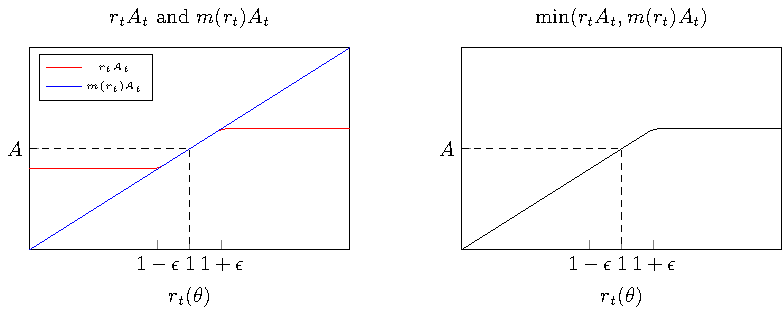
\includegraphics[page=1, scale=0.6]{clip_graph/clip_graph}
                \caption{Case $A > 0$}
            \end{figure}
            \begin{figure}[H]
                \includegraphics[page=2, scale=0.6]{clip_graph/clip_graph}
                \caption{Case $A > 0$}
            \end{figure}
        \end{center}
        % NOTE we can think of the clipped-off area as a replacement for the
        % penalty term in the original TRPO
        \framebreak
        \item Research question: how can we more precisely control penalties 
            introduced through the clipping objective?
    \end{itemize}
\end{frame}

\begin{frame}[noframenumbering, allowframebreaks]{Potential Shortcoming of PPO}
    \begin{itemize}
        \item We can separate the loss into its positive and negative
            components:
        \begin{align*}
            L^{CLIP}(\theta) &= \mathbb{E}_t\left[ 
            \min\left(r_tA_t, \text{clip}
            (r_t, 1 - \epsilon, 1 + \epsilon)A_t\right)\right]\\
            &= \mathbb{E}_t\left[ 
            \begin{cases}
                \min\left(r_t, \text{clip}
                (r_t, 1 + \epsilon)\right)A_t & A_t > 0\\
                \max\left(r_t, \text{clip}
                (r_t, 1 - \epsilon)\right)A_t & A_t < 0
            \end{cases}\right]
        \end{align*}
        \item Let:
        \begin{align*}
            r_{t, CLIP}^+ &= 
            \min\left(r_t, \text{clip}
            (r_t, 1 + \epsilon)\right)\\
            r_{t, CLIP}^- &= 
            \max\left(r_t, \text{clip}
            (r_t, 1 - \epsilon)\right)
        \end{align*}
        \item Because $\mathbb{E}_t[r_t] = 1$, we know that:
        \begin{align*}
            \mathbb{E}_t[r_{t, CLIP}^+] &< 1\\
            \mathbb{E}_t[r_{t, CLIP}^-] &> 1\\
        \end{align*}\\

        \framebreak
        \item Now, we can define the ``expected penalty contributions'' of
            positive and negative advantages:
        \begin{align*}
            1 - \mathbb{E}_t[r_{t, CLIP}^+]
        \end{align*}
        and
        \begin{align*}
            \mathbb{E}_t[r_{t, CLIP}^-] - 1
        \end{align*}
        \item Because $r_t$ and $A_t$ are not independent, these expected
            penalty contributions do not suggest actual penalty contributions.
        \item However, they can indicate inherent imbalances in the system.
    \end{itemize}
    \framebreak
    Conceptual Example
    \begin{itemize}
        \item Consider a typical example in reinforcement learning where:
            \begin{itemize}
                \item We have an agent using a continuous action
                    space (continuous control).
                \item The policy is encoded by a gaussian with state-dependent
                    means but constant standard deviation.
                % NOTE explain this carefully
            \end{itemize}
    \end{itemize}
    \framebreak
    What happens as we learn?\\
    % NOTE note that we are restrincting our view to a particular state, but
    % this happens in general across all states
    \begin{center}
        \animategraphics[scale=0.5,autoplay,loop]{15}{discrepancy}{}{}
    \end{center}
    %NOTE mention increasing discrepancy
    \framebreak
    This discrepancy also appears empirically:
    \begin{center}
        \scalebox{0.6}{%% Creator: Matplotlib, PGF backend
%%
%% To include the figure in your LaTeX document, write
%%   \input{<filename>.pgf}
%%
%% Make sure the required packages are loaded in your preamble
%%   \usepackage{pgf}
%%
%% Figures using additional raster images can only be included by \input if
%% they are in the same directory as the main LaTeX file. For loading figures
%% from other directories you can use the `import` package
%%   \usepackage{import}
%% and then include the figures with
%%   \import{<path to file>}{<filename>.pgf}
%%
%% Matplotlib used the following preamble
%%   \usepackage{fontspec}
%%   \setmainfont{DejaVu Serif}
%%   \setsansfont{DejaVu Sans}
%%   \setmonofont{DejaVu Sans Mono}
%%
\begingroup%
\makeatletter%
\begin{pgfpicture}%
\pgfpathrectangle{\pgfpointorigin}{\pgfqpoint{6.400000in}{4.800000in}}%
\pgfusepath{use as bounding box, clip}%
\begin{pgfscope}%
\pgfsetbuttcap%
\pgfsetmiterjoin%
\definecolor{currentfill}{rgb}{1.000000,1.000000,1.000000}%
\pgfsetfillcolor{currentfill}%
\pgfsetlinewidth{0.000000pt}%
\definecolor{currentstroke}{rgb}{1.000000,1.000000,1.000000}%
\pgfsetstrokecolor{currentstroke}%
\pgfsetdash{}{0pt}%
\pgfpathmoveto{\pgfqpoint{0.000000in}{0.000000in}}%
\pgfpathlineto{\pgfqpoint{6.400000in}{0.000000in}}%
\pgfpathlineto{\pgfqpoint{6.400000in}{4.800000in}}%
\pgfpathlineto{\pgfqpoint{0.000000in}{4.800000in}}%
\pgfpathclose%
\pgfusepath{fill}%
\end{pgfscope}%
\begin{pgfscope}%
\pgfsetbuttcap%
\pgfsetmiterjoin%
\definecolor{currentfill}{rgb}{1.000000,1.000000,1.000000}%
\pgfsetfillcolor{currentfill}%
\pgfsetlinewidth{0.000000pt}%
\definecolor{currentstroke}{rgb}{0.000000,0.000000,0.000000}%
\pgfsetstrokecolor{currentstroke}%
\pgfsetstrokeopacity{0.000000}%
\pgfsetdash{}{0pt}%
\pgfpathmoveto{\pgfqpoint{0.757955in}{0.582778in}}%
\pgfpathlineto{\pgfqpoint{6.215000in}{0.582778in}}%
\pgfpathlineto{\pgfqpoint{6.215000in}{4.426667in}}%
\pgfpathlineto{\pgfqpoint{0.757955in}{4.426667in}}%
\pgfpathclose%
\pgfusepath{fill}%
\end{pgfscope}%
\begin{pgfscope}%
\pgfsetbuttcap%
\pgfsetroundjoin%
\definecolor{currentfill}{rgb}{0.000000,0.000000,0.000000}%
\pgfsetfillcolor{currentfill}%
\pgfsetlinewidth{0.803000pt}%
\definecolor{currentstroke}{rgb}{0.000000,0.000000,0.000000}%
\pgfsetstrokecolor{currentstroke}%
\pgfsetdash{}{0pt}%
\pgfsys@defobject{currentmarker}{\pgfqpoint{0.000000in}{-0.048611in}}{\pgfqpoint{0.000000in}{0.000000in}}{%
\pgfpathmoveto{\pgfqpoint{0.000000in}{0.000000in}}%
\pgfpathlineto{\pgfqpoint{0.000000in}{-0.048611in}}%
\pgfusepath{stroke,fill}%
}%
\begin{pgfscope}%
\pgfsys@transformshift{1.316062in}{0.582778in}%
\pgfsys@useobject{currentmarker}{}%
\end{pgfscope}%
\end{pgfscope}%
\begin{pgfscope}%
\pgftext[x=1.316062in,y=0.485556in,,top]{\sffamily\fontsize{10.000000}{12.000000}\selectfont \(\displaystyle 2\)}%
\end{pgfscope}%
\begin{pgfscope}%
\pgfsetbuttcap%
\pgfsetroundjoin%
\definecolor{currentfill}{rgb}{0.000000,0.000000,0.000000}%
\pgfsetfillcolor{currentfill}%
\pgfsetlinewidth{0.803000pt}%
\definecolor{currentstroke}{rgb}{0.000000,0.000000,0.000000}%
\pgfsetstrokecolor{currentstroke}%
\pgfsetdash{}{0pt}%
\pgfsys@defobject{currentmarker}{\pgfqpoint{0.000000in}{-0.048611in}}{\pgfqpoint{0.000000in}{0.000000in}}{%
\pgfpathmoveto{\pgfqpoint{0.000000in}{0.000000in}}%
\pgfpathlineto{\pgfqpoint{0.000000in}{-0.048611in}}%
\pgfusepath{stroke,fill}%
}%
\begin{pgfscope}%
\pgfsys@transformshift{1.936181in}{0.582778in}%
\pgfsys@useobject{currentmarker}{}%
\end{pgfscope}%
\end{pgfscope}%
\begin{pgfscope}%
\pgftext[x=1.936181in,y=0.485556in,,top]{\sffamily\fontsize{10.000000}{12.000000}\selectfont \(\displaystyle 4\)}%
\end{pgfscope}%
\begin{pgfscope}%
\pgfsetbuttcap%
\pgfsetroundjoin%
\definecolor{currentfill}{rgb}{0.000000,0.000000,0.000000}%
\pgfsetfillcolor{currentfill}%
\pgfsetlinewidth{0.803000pt}%
\definecolor{currentstroke}{rgb}{0.000000,0.000000,0.000000}%
\pgfsetstrokecolor{currentstroke}%
\pgfsetdash{}{0pt}%
\pgfsys@defobject{currentmarker}{\pgfqpoint{0.000000in}{-0.048611in}}{\pgfqpoint{0.000000in}{0.000000in}}{%
\pgfpathmoveto{\pgfqpoint{0.000000in}{0.000000in}}%
\pgfpathlineto{\pgfqpoint{0.000000in}{-0.048611in}}%
\pgfusepath{stroke,fill}%
}%
\begin{pgfscope}%
\pgfsys@transformshift{2.556299in}{0.582778in}%
\pgfsys@useobject{currentmarker}{}%
\end{pgfscope}%
\end{pgfscope}%
\begin{pgfscope}%
\pgftext[x=2.556299in,y=0.485556in,,top]{\sffamily\fontsize{10.000000}{12.000000}\selectfont \(\displaystyle 6\)}%
\end{pgfscope}%
\begin{pgfscope}%
\pgfsetbuttcap%
\pgfsetroundjoin%
\definecolor{currentfill}{rgb}{0.000000,0.000000,0.000000}%
\pgfsetfillcolor{currentfill}%
\pgfsetlinewidth{0.803000pt}%
\definecolor{currentstroke}{rgb}{0.000000,0.000000,0.000000}%
\pgfsetstrokecolor{currentstroke}%
\pgfsetdash{}{0pt}%
\pgfsys@defobject{currentmarker}{\pgfqpoint{0.000000in}{-0.048611in}}{\pgfqpoint{0.000000in}{0.000000in}}{%
\pgfpathmoveto{\pgfqpoint{0.000000in}{0.000000in}}%
\pgfpathlineto{\pgfqpoint{0.000000in}{-0.048611in}}%
\pgfusepath{stroke,fill}%
}%
\begin{pgfscope}%
\pgfsys@transformshift{3.176418in}{0.582778in}%
\pgfsys@useobject{currentmarker}{}%
\end{pgfscope}%
\end{pgfscope}%
\begin{pgfscope}%
\pgftext[x=3.176418in,y=0.485556in,,top]{\sffamily\fontsize{10.000000}{12.000000}\selectfont \(\displaystyle 8\)}%
\end{pgfscope}%
\begin{pgfscope}%
\pgfsetbuttcap%
\pgfsetroundjoin%
\definecolor{currentfill}{rgb}{0.000000,0.000000,0.000000}%
\pgfsetfillcolor{currentfill}%
\pgfsetlinewidth{0.803000pt}%
\definecolor{currentstroke}{rgb}{0.000000,0.000000,0.000000}%
\pgfsetstrokecolor{currentstroke}%
\pgfsetdash{}{0pt}%
\pgfsys@defobject{currentmarker}{\pgfqpoint{0.000000in}{-0.048611in}}{\pgfqpoint{0.000000in}{0.000000in}}{%
\pgfpathmoveto{\pgfqpoint{0.000000in}{0.000000in}}%
\pgfpathlineto{\pgfqpoint{0.000000in}{-0.048611in}}%
\pgfusepath{stroke,fill}%
}%
\begin{pgfscope}%
\pgfsys@transformshift{3.796537in}{0.582778in}%
\pgfsys@useobject{currentmarker}{}%
\end{pgfscope}%
\end{pgfscope}%
\begin{pgfscope}%
\pgftext[x=3.796537in,y=0.485556in,,top]{\sffamily\fontsize{10.000000}{12.000000}\selectfont \(\displaystyle 10\)}%
\end{pgfscope}%
\begin{pgfscope}%
\pgfsetbuttcap%
\pgfsetroundjoin%
\definecolor{currentfill}{rgb}{0.000000,0.000000,0.000000}%
\pgfsetfillcolor{currentfill}%
\pgfsetlinewidth{0.803000pt}%
\definecolor{currentstroke}{rgb}{0.000000,0.000000,0.000000}%
\pgfsetstrokecolor{currentstroke}%
\pgfsetdash{}{0pt}%
\pgfsys@defobject{currentmarker}{\pgfqpoint{0.000000in}{-0.048611in}}{\pgfqpoint{0.000000in}{0.000000in}}{%
\pgfpathmoveto{\pgfqpoint{0.000000in}{0.000000in}}%
\pgfpathlineto{\pgfqpoint{0.000000in}{-0.048611in}}%
\pgfusepath{stroke,fill}%
}%
\begin{pgfscope}%
\pgfsys@transformshift{4.416656in}{0.582778in}%
\pgfsys@useobject{currentmarker}{}%
\end{pgfscope}%
\end{pgfscope}%
\begin{pgfscope}%
\pgftext[x=4.416656in,y=0.485556in,,top]{\sffamily\fontsize{10.000000}{12.000000}\selectfont \(\displaystyle 12\)}%
\end{pgfscope}%
\begin{pgfscope}%
\pgfsetbuttcap%
\pgfsetroundjoin%
\definecolor{currentfill}{rgb}{0.000000,0.000000,0.000000}%
\pgfsetfillcolor{currentfill}%
\pgfsetlinewidth{0.803000pt}%
\definecolor{currentstroke}{rgb}{0.000000,0.000000,0.000000}%
\pgfsetstrokecolor{currentstroke}%
\pgfsetdash{}{0pt}%
\pgfsys@defobject{currentmarker}{\pgfqpoint{0.000000in}{-0.048611in}}{\pgfqpoint{0.000000in}{0.000000in}}{%
\pgfpathmoveto{\pgfqpoint{0.000000in}{0.000000in}}%
\pgfpathlineto{\pgfqpoint{0.000000in}{-0.048611in}}%
\pgfusepath{stroke,fill}%
}%
\begin{pgfscope}%
\pgfsys@transformshift{5.036774in}{0.582778in}%
\pgfsys@useobject{currentmarker}{}%
\end{pgfscope}%
\end{pgfscope}%
\begin{pgfscope}%
\pgftext[x=5.036774in,y=0.485556in,,top]{\sffamily\fontsize{10.000000}{12.000000}\selectfont \(\displaystyle 14\)}%
\end{pgfscope}%
\begin{pgfscope}%
\pgfsetbuttcap%
\pgfsetroundjoin%
\definecolor{currentfill}{rgb}{0.000000,0.000000,0.000000}%
\pgfsetfillcolor{currentfill}%
\pgfsetlinewidth{0.803000pt}%
\definecolor{currentstroke}{rgb}{0.000000,0.000000,0.000000}%
\pgfsetstrokecolor{currentstroke}%
\pgfsetdash{}{0pt}%
\pgfsys@defobject{currentmarker}{\pgfqpoint{0.000000in}{-0.048611in}}{\pgfqpoint{0.000000in}{0.000000in}}{%
\pgfpathmoveto{\pgfqpoint{0.000000in}{0.000000in}}%
\pgfpathlineto{\pgfqpoint{0.000000in}{-0.048611in}}%
\pgfusepath{stroke,fill}%
}%
\begin{pgfscope}%
\pgfsys@transformshift{5.656893in}{0.582778in}%
\pgfsys@useobject{currentmarker}{}%
\end{pgfscope}%
\end{pgfscope}%
\begin{pgfscope}%
\pgftext[x=5.656893in,y=0.485556in,,top]{\sffamily\fontsize{10.000000}{12.000000}\selectfont \(\displaystyle 16\)}%
\end{pgfscope}%
\begin{pgfscope}%
\pgftext[x=3.486477in,y=0.295587in,,top]{\sffamily\fontsize{10.000000}{12.000000}\selectfont Number of Iterations}%
\end{pgfscope}%
\begin{pgfscope}%
\pgfsetbuttcap%
\pgfsetroundjoin%
\definecolor{currentfill}{rgb}{0.000000,0.000000,0.000000}%
\pgfsetfillcolor{currentfill}%
\pgfsetlinewidth{0.803000pt}%
\definecolor{currentstroke}{rgb}{0.000000,0.000000,0.000000}%
\pgfsetstrokecolor{currentstroke}%
\pgfsetdash{}{0pt}%
\pgfsys@defobject{currentmarker}{\pgfqpoint{-0.048611in}{0.000000in}}{\pgfqpoint{0.000000in}{0.000000in}}{%
\pgfpathmoveto{\pgfqpoint{0.000000in}{0.000000in}}%
\pgfpathlineto{\pgfqpoint{-0.048611in}{0.000000in}}%
\pgfusepath{stroke,fill}%
}%
\begin{pgfscope}%
\pgfsys@transformshift{0.757955in}{0.711952in}%
\pgfsys@useobject{currentmarker}{}%
\end{pgfscope}%
\end{pgfscope}%
\begin{pgfscope}%
\pgftext[x=0.344374in,y=0.659191in,left,base]{\sffamily\fontsize{10.000000}{12.000000}\selectfont \(\displaystyle 0.000\)}%
\end{pgfscope}%
\begin{pgfscope}%
\pgfsetbuttcap%
\pgfsetroundjoin%
\definecolor{currentfill}{rgb}{0.000000,0.000000,0.000000}%
\pgfsetfillcolor{currentfill}%
\pgfsetlinewidth{0.803000pt}%
\definecolor{currentstroke}{rgb}{0.000000,0.000000,0.000000}%
\pgfsetstrokecolor{currentstroke}%
\pgfsetdash{}{0pt}%
\pgfsys@defobject{currentmarker}{\pgfqpoint{-0.048611in}{0.000000in}}{\pgfqpoint{0.000000in}{0.000000in}}{%
\pgfpathmoveto{\pgfqpoint{0.000000in}{0.000000in}}%
\pgfpathlineto{\pgfqpoint{-0.048611in}{0.000000in}}%
\pgfusepath{stroke,fill}%
}%
\begin{pgfscope}%
\pgfsys@transformshift{0.757955in}{1.532636in}%
\pgfsys@useobject{currentmarker}{}%
\end{pgfscope}%
\end{pgfscope}%
\begin{pgfscope}%
\pgftext[x=0.344374in,y=1.479874in,left,base]{\sffamily\fontsize{10.000000}{12.000000}\selectfont \(\displaystyle 0.005\)}%
\end{pgfscope}%
\begin{pgfscope}%
\pgfsetbuttcap%
\pgfsetroundjoin%
\definecolor{currentfill}{rgb}{0.000000,0.000000,0.000000}%
\pgfsetfillcolor{currentfill}%
\pgfsetlinewidth{0.803000pt}%
\definecolor{currentstroke}{rgb}{0.000000,0.000000,0.000000}%
\pgfsetstrokecolor{currentstroke}%
\pgfsetdash{}{0pt}%
\pgfsys@defobject{currentmarker}{\pgfqpoint{-0.048611in}{0.000000in}}{\pgfqpoint{0.000000in}{0.000000in}}{%
\pgfpathmoveto{\pgfqpoint{0.000000in}{0.000000in}}%
\pgfpathlineto{\pgfqpoint{-0.048611in}{0.000000in}}%
\pgfusepath{stroke,fill}%
}%
\begin{pgfscope}%
\pgfsys@transformshift{0.757955in}{2.353319in}%
\pgfsys@useobject{currentmarker}{}%
\end{pgfscope}%
\end{pgfscope}%
\begin{pgfscope}%
\pgftext[x=0.344374in,y=2.300557in,left,base]{\sffamily\fontsize{10.000000}{12.000000}\selectfont \(\displaystyle 0.010\)}%
\end{pgfscope}%
\begin{pgfscope}%
\pgfsetbuttcap%
\pgfsetroundjoin%
\definecolor{currentfill}{rgb}{0.000000,0.000000,0.000000}%
\pgfsetfillcolor{currentfill}%
\pgfsetlinewidth{0.803000pt}%
\definecolor{currentstroke}{rgb}{0.000000,0.000000,0.000000}%
\pgfsetstrokecolor{currentstroke}%
\pgfsetdash{}{0pt}%
\pgfsys@defobject{currentmarker}{\pgfqpoint{-0.048611in}{0.000000in}}{\pgfqpoint{0.000000in}{0.000000in}}{%
\pgfpathmoveto{\pgfqpoint{0.000000in}{0.000000in}}%
\pgfpathlineto{\pgfqpoint{-0.048611in}{0.000000in}}%
\pgfusepath{stroke,fill}%
}%
\begin{pgfscope}%
\pgfsys@transformshift{0.757955in}{3.174002in}%
\pgfsys@useobject{currentmarker}{}%
\end{pgfscope}%
\end{pgfscope}%
\begin{pgfscope}%
\pgftext[x=0.344374in,y=3.121241in,left,base]{\sffamily\fontsize{10.000000}{12.000000}\selectfont \(\displaystyle 0.015\)}%
\end{pgfscope}%
\begin{pgfscope}%
\pgfsetbuttcap%
\pgfsetroundjoin%
\definecolor{currentfill}{rgb}{0.000000,0.000000,0.000000}%
\pgfsetfillcolor{currentfill}%
\pgfsetlinewidth{0.803000pt}%
\definecolor{currentstroke}{rgb}{0.000000,0.000000,0.000000}%
\pgfsetstrokecolor{currentstroke}%
\pgfsetdash{}{0pt}%
\pgfsys@defobject{currentmarker}{\pgfqpoint{-0.048611in}{0.000000in}}{\pgfqpoint{0.000000in}{0.000000in}}{%
\pgfpathmoveto{\pgfqpoint{0.000000in}{0.000000in}}%
\pgfpathlineto{\pgfqpoint{-0.048611in}{0.000000in}}%
\pgfusepath{stroke,fill}%
}%
\begin{pgfscope}%
\pgfsys@transformshift{0.757955in}{3.994686in}%
\pgfsys@useobject{currentmarker}{}%
\end{pgfscope}%
\end{pgfscope}%
\begin{pgfscope}%
\pgftext[x=0.344374in,y=3.941924in,left,base]{\sffamily\fontsize{10.000000}{12.000000}\selectfont \(\displaystyle 0.020\)}%
\end{pgfscope}%
\begin{pgfscope}%
\pgftext[x=0.288818in,y=2.504722in,,bottom,rotate=90.000000]{\sffamily\fontsize{10.000000}{12.000000}\selectfont Proportional Contribution}%
\end{pgfscope}%
\begin{pgfscope}%
\pgfpathrectangle{\pgfqpoint{0.757955in}{0.582778in}}{\pgfqpoint{5.457045in}{3.843889in}}%
\pgfusepath{clip}%
\pgfsetrectcap%
\pgfsetroundjoin%
\pgfsetlinewidth{1.505625pt}%
\definecolor{currentstroke}{rgb}{0.000000,0.000000,0.000000}%
\pgfsetstrokecolor{currentstroke}%
\pgfsetdash{}{0pt}%
\pgfpathmoveto{\pgfqpoint{1.006002in}{3.533677in}}%
\pgfpathlineto{\pgfqpoint{1.316062in}{4.251944in}}%
\pgfpathlineto{\pgfqpoint{1.626121in}{3.569340in}}%
\pgfpathlineto{\pgfqpoint{1.936181in}{2.765420in}}%
\pgfpathlineto{\pgfqpoint{2.246240in}{1.871555in}}%
\pgfpathlineto{\pgfqpoint{2.556299in}{1.553503in}}%
\pgfpathlineto{\pgfqpoint{2.866359in}{1.431250in}}%
\pgfpathlineto{\pgfqpoint{3.176418in}{1.416363in}}%
\pgfpathlineto{\pgfqpoint{3.486477in}{1.508206in}}%
\pgfpathlineto{\pgfqpoint{3.796537in}{1.204933in}}%
\pgfpathlineto{\pgfqpoint{4.106596in}{1.108082in}}%
\pgfpathlineto{\pgfqpoint{4.416656in}{0.865045in}}%
\pgfpathlineto{\pgfqpoint{4.726715in}{0.938093in}}%
\pgfpathlineto{\pgfqpoint{5.036774in}{0.893178in}}%
\pgfpathlineto{\pgfqpoint{5.346834in}{0.949233in}}%
\pgfpathlineto{\pgfqpoint{5.656893in}{0.924012in}}%
\pgfpathlineto{\pgfqpoint{5.966952in}{0.822725in}}%
\pgfusepath{stroke}%
\end{pgfscope}%
\begin{pgfscope}%
\pgfpathrectangle{\pgfqpoint{0.757955in}{0.582778in}}{\pgfqpoint{5.457045in}{3.843889in}}%
\pgfusepath{clip}%
\pgfsetrectcap%
\pgfsetroundjoin%
\pgfsetlinewidth{1.505625pt}%
\definecolor{currentstroke}{rgb}{0.000000,0.000000,0.000000}%
\pgfsetstrokecolor{currentstroke}%
\pgfsetdash{}{0pt}%
\pgfpathmoveto{\pgfqpoint{1.006002in}{2.308621in}}%
\pgfpathlineto{\pgfqpoint{1.316062in}{2.810948in}}%
\pgfpathlineto{\pgfqpoint{1.626121in}{2.537687in}}%
\pgfpathlineto{\pgfqpoint{1.936181in}{1.963244in}}%
\pgfpathlineto{\pgfqpoint{2.246240in}{1.341394in}}%
\pgfpathlineto{\pgfqpoint{2.556299in}{1.120764in}}%
\pgfpathlineto{\pgfqpoint{2.866359in}{1.080235in}}%
\pgfpathlineto{\pgfqpoint{3.176418in}{1.067171in}}%
\pgfpathlineto{\pgfqpoint{3.486477in}{1.170607in}}%
\pgfpathlineto{\pgfqpoint{3.796537in}{0.954125in}}%
\pgfpathlineto{\pgfqpoint{4.106596in}{0.909487in}}%
\pgfpathlineto{\pgfqpoint{4.416656in}{0.773956in}}%
\pgfpathlineto{\pgfqpoint{4.726715in}{0.804567in}}%
\pgfpathlineto{\pgfqpoint{5.036774in}{0.817436in}}%
\pgfpathlineto{\pgfqpoint{5.346834in}{0.809981in}}%
\pgfpathlineto{\pgfqpoint{5.656893in}{0.815870in}}%
\pgfpathlineto{\pgfqpoint{5.966952in}{0.757500in}}%
\pgfusepath{stroke}%
\end{pgfscope}%
\begin{pgfscope}%
\pgfsetrectcap%
\pgfsetmiterjoin%
\pgfsetlinewidth{0.803000pt}%
\definecolor{currentstroke}{rgb}{0.000000,0.000000,0.000000}%
\pgfsetstrokecolor{currentstroke}%
\pgfsetdash{}{0pt}%
\pgfpathmoveto{\pgfqpoint{0.757955in}{0.582778in}}%
\pgfpathlineto{\pgfqpoint{0.757955in}{4.426667in}}%
\pgfusepath{stroke}%
\end{pgfscope}%
\begin{pgfscope}%
\pgfsetrectcap%
\pgfsetmiterjoin%
\pgfsetlinewidth{0.803000pt}%
\definecolor{currentstroke}{rgb}{0.000000,0.000000,0.000000}%
\pgfsetstrokecolor{currentstroke}%
\pgfsetdash{}{0pt}%
\pgfpathmoveto{\pgfqpoint{6.215000in}{0.582778in}}%
\pgfpathlineto{\pgfqpoint{6.215000in}{4.426667in}}%
\pgfusepath{stroke}%
\end{pgfscope}%
\begin{pgfscope}%
\pgfsetrectcap%
\pgfsetmiterjoin%
\pgfsetlinewidth{0.803000pt}%
\definecolor{currentstroke}{rgb}{0.000000,0.000000,0.000000}%
\pgfsetstrokecolor{currentstroke}%
\pgfsetdash{}{0pt}%
\pgfpathmoveto{\pgfqpoint{0.757955in}{0.582778in}}%
\pgfpathlineto{\pgfqpoint{6.215000in}{0.582778in}}%
\pgfusepath{stroke}%
\end{pgfscope}%
\begin{pgfscope}%
\pgfsetrectcap%
\pgfsetmiterjoin%
\pgfsetlinewidth{0.803000pt}%
\definecolor{currentstroke}{rgb}{0.000000,0.000000,0.000000}%
\pgfsetstrokecolor{currentstroke}%
\pgfsetdash{}{0pt}%
\pgfpathmoveto{\pgfqpoint{0.757955in}{4.426667in}}%
\pgfpathlineto{\pgfqpoint{6.215000in}{4.426667in}}%
\pgfusepath{stroke}%
\end{pgfscope}%
\begin{pgfscope}%
\pgftext[x=3.486477in,y=4.510000in,,base]{\sffamily\fontsize{12.000000}{14.400000}\selectfont Expected Penalty Contributions}%
\end{pgfscope}%
\begin{pgfscope}%
\pgfsetbuttcap%
\pgfsetmiterjoin%
\definecolor{currentfill}{rgb}{1.000000,1.000000,1.000000}%
\pgfsetfillcolor{currentfill}%
\pgfsetfillopacity{0.800000}%
\pgfsetlinewidth{1.003750pt}%
\definecolor{currentstroke}{rgb}{0.800000,0.800000,0.800000}%
\pgfsetstrokecolor{currentstroke}%
\pgfsetstrokeopacity{0.800000}%
\pgfsetdash{}{0pt}%
\pgfpathmoveto{\pgfqpoint{4.796785in}{3.818027in}}%
\pgfpathlineto{\pgfqpoint{6.117778in}{3.818027in}}%
\pgfpathquadraticcurveto{\pgfqpoint{6.145556in}{3.818027in}}{\pgfqpoint{6.145556in}{3.845804in}}%
\pgfpathlineto{\pgfqpoint{6.145556in}{4.329444in}}%
\pgfpathquadraticcurveto{\pgfqpoint{6.145556in}{4.357222in}}{\pgfqpoint{6.117778in}{4.357222in}}%
\pgfpathlineto{\pgfqpoint{4.796785in}{4.357222in}}%
\pgfpathquadraticcurveto{\pgfqpoint{4.769007in}{4.357222in}}{\pgfqpoint{4.769007in}{4.329444in}}%
\pgfpathlineto{\pgfqpoint{4.769007in}{3.845804in}}%
\pgfpathquadraticcurveto{\pgfqpoint{4.769007in}{3.818027in}}{\pgfqpoint{4.796785in}{3.818027in}}%
\pgfpathclose%
\pgfusepath{stroke,fill}%
\end{pgfscope}%
\begin{pgfscope}%
\pgfsetrectcap%
\pgfsetroundjoin%
\pgfsetlinewidth{1.505625pt}%
\definecolor{currentstroke}{rgb}{0.000000,0.000000,0.000000}%
\pgfsetstrokecolor{currentstroke}%
\pgfsetdash{}{0pt}%
\pgfpathmoveto{\pgfqpoint{4.824562in}{4.230679in}}%
\pgfpathlineto{\pgfqpoint{5.102340in}{4.230679in}}%
\pgfusepath{stroke}%
\end{pgfscope}%
\begin{pgfscope}%
\pgftext[x=5.213451in,y=4.182068in,left,base]{\sffamily\fontsize{10.000000}{12.000000}\selectfont \(\displaystyle 1 - E[r_{t, CLIP}^+]\)}%
\end{pgfscope}%
\begin{pgfscope}%
\pgfsetrectcap%
\pgfsetroundjoin%
\pgfsetlinewidth{1.505625pt}%
\definecolor{currentstroke}{rgb}{0.000000,0.000000,0.000000}%
\pgfsetstrokecolor{currentstroke}%
\pgfsetdash{}{0pt}%
\pgfpathmoveto{\pgfqpoint{4.824562in}{3.981915in}}%
\pgfpathlineto{\pgfqpoint{5.102340in}{3.981915in}}%
\pgfusepath{stroke}%
\end{pgfscope}%
\begin{pgfscope}%
\pgftext[x=5.213451in,y=3.933303in,left,base]{\sffamily\fontsize{10.000000}{12.000000}\selectfont \(\displaystyle E[r_{t, CLIP}^-] - 1\)}%
\end{pgfscope}%
\end{pgfpicture}%
\makeatother%
\endgroup%
}\\
    \end{center}
    \framebreak
    \begin{itemize}
        \item The discrepancy between positive and negative penalty
            contributions is unintentional and highly dependent on the shape of
            the distribution.
        \item The goal of this project is to investigate the effects of
            controlling this discrepancy directly.
    \end{itemize}
\end{frame}

\begin{frame}[noframenumbering, allowframebreaks]{Idea}
    \begin{itemize}
        \item In the gaussian example, we can precisely calculate the
            discrepancy at a particular state using the equation:
        \scriptsize
        \begin{align*}
            (1 - E[r_{t, CLIP}^{+}]) - (E[r_{t, CLIP}^{-}] - 1)
            &=
            \epsilon
            + 
            (1 - \epsilon)
            \int_{x^{-}}^{x^{+}}p(\mu_{old}, x)dx
            \\
            &-\left(\int_{x^{-}}^{x^{+}}p(\mu, x)dx 
            +2\epsilon
            \int_{x^{+}}^{\infty}p(\mu_{old}, x)dx\right)\\
        \end{align*}
        \normalsize
        where
        \begin{align*}
            x^{+} &=
            \frac{(\mu^2 - \mu_{old}^2)
                + 2\sigma^2\ln\left(1 + \epsilon\right)}
                {2(\mu - \mu_{old})}
        \end{align*}
        and
        \begin{align*}
            x^{-} &=
            \frac{(\mu^2 - \mu_{old}^2)
                + 2\sigma^2\ln\left(1 - \epsilon\right)}
                {2(\mu - \mu_{old})}
        \end{align*}
        \framebreak
        \item If we want to minimize this using $\epsilon$, this equation
            doesn't give us very much control.
        \item Generalizing to two $\epsilon$ by redefining the clipping
            function as $\text{clip} (r_t, 1 - \epsilon^-, 1 + \epsilon^+)$:
        \scriptsize
        \begin{align*}
            (1 - E[r_{t, CLIP}^{+}]) - (E[r_{t, CLIP}^{-}] - 1)
            &=
            \epsilon^-
            + 
            (1 - \epsilon^-)
            \int_{x^{-}}^{x^{+}}p(\mu_{old}, x)dx
            \\
            &-\left(\int_{x^{-}}^{x^{+}}p(\mu, x)dx 
            +(\epsilon^+ + \epsilon^-)
            \int_{x^{+}}^{\infty}p(\mu_{old}, x)dx\right)\\
        \end{align*}
        % NOTE increasing e^- will tend to increase the value, and decreasing
        % e^+ will tend to decrease the value
        \normalsize
        \item We can also define the total expected penalty contributions:
        \tiny
        \begin{align*}
            (1 - E[r_{t, CLIP}^{+}]) + (E[r_{t, CLIP}^{-}] - 1)
            &=
            2\int_{x^{+}}^{\infty}
            p(\mu, x)
            dx -
            (2 + \epsilon^+ - \epsilon^-)
            \int_{x^{+}}^{\infty}p(\mu_{old}, x)dx\\
            &-
            \epsilon^-
            - 
            (1 - \epsilon^-)
            \int_{x^{-}}^{x^{+}}p(\mu_{old}, x)dx + 
            \int_{x^{-}}^{x^{+}}p(\mu, x)dx
            \\
        \end{align*}
        \normalsize
        \framebreak
        \item The new algorithm is identical to PPO, except we use two
            $\epsilon$, and at the end of every model update, we optimize
            $\epsilon^-$ and $\epsilon^+$ so that:
        \begin{itemize}
            \item $(1 - E[r_{t, CLIP}^{+}]) - (E[r_{t, CLIP}^{-}] - 1)$ is
                minimized.
            \item $(1 - E[r_{t, CLIP}^{+}]) + (E[r_{t, CLIP}^{-}] - 1)$ remains
                the same.
        \end{itemize}
    \end{itemize}
\end{frame}

\begin{frame}[noframenumbering, allowframebreaks]{Results}
    \begin{itemize}
        \item Overall, we observed approximately the same performance or modest
            improvements.
        \item The optimization was always successful in reducing the empirical
            discrepancy.
    \end{itemize}
    \framebreak
    Example: Walker2d-v2 environment
    \scalebox{0.6}{%% Creator: Matplotlib, PGF backend
%%
%% To include the figure in your LaTeX document, write
%%   \input{<filename>.pgf}
%%
%% Make sure the required packages are loaded in your preamble
%%   \usepackage{pgf}
%%
%% Figures using additional raster images can only be included by \input if
%% they are in the same directory as the main LaTeX file. For loading figures
%% from other directories you can use the `import` package
%%   \usepackage{import}
%% and then include the figures with
%%   \import{<path to file>}{<filename>.pgf}
%%
%% Matplotlib used the following preamble
%%   \usepackage{fontspec}
%%   \setmainfont{DejaVu Serif}
%%   \setsansfont{DejaVu Sans}
%%   \setmonofont{DejaVu Sans Mono}
%%
\begingroup%
\makeatletter%
\begin{pgfpicture}%
\pgfpathrectangle{\pgfpointorigin}{\pgfqpoint{6.400000in}{4.800000in}}%
\pgfusepath{use as bounding box, clip}%
\begin{pgfscope}%
\pgfsetbuttcap%
\pgfsetmiterjoin%
\definecolor{currentfill}{rgb}{1.000000,1.000000,1.000000}%
\pgfsetfillcolor{currentfill}%
\pgfsetlinewidth{0.000000pt}%
\definecolor{currentstroke}{rgb}{1.000000,1.000000,1.000000}%
\pgfsetstrokecolor{currentstroke}%
\pgfsetdash{}{0pt}%
\pgfpathmoveto{\pgfqpoint{0.000000in}{0.000000in}}%
\pgfpathlineto{\pgfqpoint{6.400000in}{0.000000in}}%
\pgfpathlineto{\pgfqpoint{6.400000in}{4.800000in}}%
\pgfpathlineto{\pgfqpoint{0.000000in}{4.800000in}}%
\pgfpathclose%
\pgfusepath{fill}%
\end{pgfscope}%
\begin{pgfscope}%
\pgfsetbuttcap%
\pgfsetmiterjoin%
\definecolor{currentfill}{rgb}{1.000000,1.000000,1.000000}%
\pgfsetfillcolor{currentfill}%
\pgfsetlinewidth{0.000000pt}%
\definecolor{currentstroke}{rgb}{0.000000,0.000000,0.000000}%
\pgfsetstrokecolor{currentstroke}%
\pgfsetstrokeopacity{0.000000}%
\pgfsetdash{}{0pt}%
\pgfpathmoveto{\pgfqpoint{0.757955in}{2.907778in}}%
\pgfpathlineto{\pgfqpoint{6.215000in}{2.907778in}}%
\pgfpathlineto{\pgfqpoint{6.215000in}{4.426667in}}%
\pgfpathlineto{\pgfqpoint{0.757955in}{4.426667in}}%
\pgfpathclose%
\pgfusepath{fill}%
\end{pgfscope}%
\begin{pgfscope}%
\pgfsetbuttcap%
\pgfsetroundjoin%
\definecolor{currentfill}{rgb}{0.000000,0.000000,0.000000}%
\pgfsetfillcolor{currentfill}%
\pgfsetlinewidth{0.803000pt}%
\definecolor{currentstroke}{rgb}{0.000000,0.000000,0.000000}%
\pgfsetstrokecolor{currentstroke}%
\pgfsetdash{}{0pt}%
\pgfsys@defobject{currentmarker}{\pgfqpoint{0.000000in}{-0.048611in}}{\pgfqpoint{0.000000in}{0.000000in}}{%
\pgfpathmoveto{\pgfqpoint{0.000000in}{0.000000in}}%
\pgfpathlineto{\pgfqpoint{0.000000in}{-0.048611in}}%
\pgfusepath{stroke,fill}%
}%
\begin{pgfscope}%
\pgfsys@transformshift{1.327175in}{2.907778in}%
\pgfsys@useobject{currentmarker}{}%
\end{pgfscope}%
\end{pgfscope}%
\begin{pgfscope}%
\pgftext[x=1.327175in,y=2.810556in,,top]{\sffamily\fontsize{10.000000}{12.000000}\selectfont \(\displaystyle 25000\)}%
\end{pgfscope}%
\begin{pgfscope}%
\pgfsetbuttcap%
\pgfsetroundjoin%
\definecolor{currentfill}{rgb}{0.000000,0.000000,0.000000}%
\pgfsetfillcolor{currentfill}%
\pgfsetlinewidth{0.803000pt}%
\definecolor{currentstroke}{rgb}{0.000000,0.000000,0.000000}%
\pgfsetstrokecolor{currentstroke}%
\pgfsetdash{}{0pt}%
\pgfsys@defobject{currentmarker}{\pgfqpoint{0.000000in}{-0.048611in}}{\pgfqpoint{0.000000in}{0.000000in}}{%
\pgfpathmoveto{\pgfqpoint{0.000000in}{0.000000in}}%
\pgfpathlineto{\pgfqpoint{0.000000in}{-0.048611in}}%
\pgfusepath{stroke,fill}%
}%
\begin{pgfscope}%
\pgfsys@transformshift{1.958542in}{2.907778in}%
\pgfsys@useobject{currentmarker}{}%
\end{pgfscope}%
\end{pgfscope}%
\begin{pgfscope}%
\pgftext[x=1.958542in,y=2.810556in,,top]{\sffamily\fontsize{10.000000}{12.000000}\selectfont \(\displaystyle 50000\)}%
\end{pgfscope}%
\begin{pgfscope}%
\pgfsetbuttcap%
\pgfsetroundjoin%
\definecolor{currentfill}{rgb}{0.000000,0.000000,0.000000}%
\pgfsetfillcolor{currentfill}%
\pgfsetlinewidth{0.803000pt}%
\definecolor{currentstroke}{rgb}{0.000000,0.000000,0.000000}%
\pgfsetstrokecolor{currentstroke}%
\pgfsetdash{}{0pt}%
\pgfsys@defobject{currentmarker}{\pgfqpoint{0.000000in}{-0.048611in}}{\pgfqpoint{0.000000in}{0.000000in}}{%
\pgfpathmoveto{\pgfqpoint{0.000000in}{0.000000in}}%
\pgfpathlineto{\pgfqpoint{0.000000in}{-0.048611in}}%
\pgfusepath{stroke,fill}%
}%
\begin{pgfscope}%
\pgfsys@transformshift{2.589910in}{2.907778in}%
\pgfsys@useobject{currentmarker}{}%
\end{pgfscope}%
\end{pgfscope}%
\begin{pgfscope}%
\pgftext[x=2.589910in,y=2.810556in,,top]{\sffamily\fontsize{10.000000}{12.000000}\selectfont \(\displaystyle 75000\)}%
\end{pgfscope}%
\begin{pgfscope}%
\pgfsetbuttcap%
\pgfsetroundjoin%
\definecolor{currentfill}{rgb}{0.000000,0.000000,0.000000}%
\pgfsetfillcolor{currentfill}%
\pgfsetlinewidth{0.803000pt}%
\definecolor{currentstroke}{rgb}{0.000000,0.000000,0.000000}%
\pgfsetstrokecolor{currentstroke}%
\pgfsetdash{}{0pt}%
\pgfsys@defobject{currentmarker}{\pgfqpoint{0.000000in}{-0.048611in}}{\pgfqpoint{0.000000in}{0.000000in}}{%
\pgfpathmoveto{\pgfqpoint{0.000000in}{0.000000in}}%
\pgfpathlineto{\pgfqpoint{0.000000in}{-0.048611in}}%
\pgfusepath{stroke,fill}%
}%
\begin{pgfscope}%
\pgfsys@transformshift{3.221278in}{2.907778in}%
\pgfsys@useobject{currentmarker}{}%
\end{pgfscope}%
\end{pgfscope}%
\begin{pgfscope}%
\pgftext[x=3.221278in,y=2.810556in,,top]{\sffamily\fontsize{10.000000}{12.000000}\selectfont \(\displaystyle 100000\)}%
\end{pgfscope}%
\begin{pgfscope}%
\pgfsetbuttcap%
\pgfsetroundjoin%
\definecolor{currentfill}{rgb}{0.000000,0.000000,0.000000}%
\pgfsetfillcolor{currentfill}%
\pgfsetlinewidth{0.803000pt}%
\definecolor{currentstroke}{rgb}{0.000000,0.000000,0.000000}%
\pgfsetstrokecolor{currentstroke}%
\pgfsetdash{}{0pt}%
\pgfsys@defobject{currentmarker}{\pgfqpoint{0.000000in}{-0.048611in}}{\pgfqpoint{0.000000in}{0.000000in}}{%
\pgfpathmoveto{\pgfqpoint{0.000000in}{0.000000in}}%
\pgfpathlineto{\pgfqpoint{0.000000in}{-0.048611in}}%
\pgfusepath{stroke,fill}%
}%
\begin{pgfscope}%
\pgfsys@transformshift{3.852645in}{2.907778in}%
\pgfsys@useobject{currentmarker}{}%
\end{pgfscope}%
\end{pgfscope}%
\begin{pgfscope}%
\pgftext[x=3.852645in,y=2.810556in,,top]{\sffamily\fontsize{10.000000}{12.000000}\selectfont \(\displaystyle 125000\)}%
\end{pgfscope}%
\begin{pgfscope}%
\pgfsetbuttcap%
\pgfsetroundjoin%
\definecolor{currentfill}{rgb}{0.000000,0.000000,0.000000}%
\pgfsetfillcolor{currentfill}%
\pgfsetlinewidth{0.803000pt}%
\definecolor{currentstroke}{rgb}{0.000000,0.000000,0.000000}%
\pgfsetstrokecolor{currentstroke}%
\pgfsetdash{}{0pt}%
\pgfsys@defobject{currentmarker}{\pgfqpoint{0.000000in}{-0.048611in}}{\pgfqpoint{0.000000in}{0.000000in}}{%
\pgfpathmoveto{\pgfqpoint{0.000000in}{0.000000in}}%
\pgfpathlineto{\pgfqpoint{0.000000in}{-0.048611in}}%
\pgfusepath{stroke,fill}%
}%
\begin{pgfscope}%
\pgfsys@transformshift{4.484013in}{2.907778in}%
\pgfsys@useobject{currentmarker}{}%
\end{pgfscope}%
\end{pgfscope}%
\begin{pgfscope}%
\pgftext[x=4.484013in,y=2.810556in,,top]{\sffamily\fontsize{10.000000}{12.000000}\selectfont \(\displaystyle 150000\)}%
\end{pgfscope}%
\begin{pgfscope}%
\pgfsetbuttcap%
\pgfsetroundjoin%
\definecolor{currentfill}{rgb}{0.000000,0.000000,0.000000}%
\pgfsetfillcolor{currentfill}%
\pgfsetlinewidth{0.803000pt}%
\definecolor{currentstroke}{rgb}{0.000000,0.000000,0.000000}%
\pgfsetstrokecolor{currentstroke}%
\pgfsetdash{}{0pt}%
\pgfsys@defobject{currentmarker}{\pgfqpoint{0.000000in}{-0.048611in}}{\pgfqpoint{0.000000in}{0.000000in}}{%
\pgfpathmoveto{\pgfqpoint{0.000000in}{0.000000in}}%
\pgfpathlineto{\pgfqpoint{0.000000in}{-0.048611in}}%
\pgfusepath{stroke,fill}%
}%
\begin{pgfscope}%
\pgfsys@transformshift{5.115381in}{2.907778in}%
\pgfsys@useobject{currentmarker}{}%
\end{pgfscope}%
\end{pgfscope}%
\begin{pgfscope}%
\pgftext[x=5.115381in,y=2.810556in,,top]{\sffamily\fontsize{10.000000}{12.000000}\selectfont \(\displaystyle 175000\)}%
\end{pgfscope}%
\begin{pgfscope}%
\pgfsetbuttcap%
\pgfsetroundjoin%
\definecolor{currentfill}{rgb}{0.000000,0.000000,0.000000}%
\pgfsetfillcolor{currentfill}%
\pgfsetlinewidth{0.803000pt}%
\definecolor{currentstroke}{rgb}{0.000000,0.000000,0.000000}%
\pgfsetstrokecolor{currentstroke}%
\pgfsetdash{}{0pt}%
\pgfsys@defobject{currentmarker}{\pgfqpoint{0.000000in}{-0.048611in}}{\pgfqpoint{0.000000in}{0.000000in}}{%
\pgfpathmoveto{\pgfqpoint{0.000000in}{0.000000in}}%
\pgfpathlineto{\pgfqpoint{0.000000in}{-0.048611in}}%
\pgfusepath{stroke,fill}%
}%
\begin{pgfscope}%
\pgfsys@transformshift{5.746748in}{2.907778in}%
\pgfsys@useobject{currentmarker}{}%
\end{pgfscope}%
\end{pgfscope}%
\begin{pgfscope}%
\pgftext[x=5.746748in,y=2.810556in,,top]{\sffamily\fontsize{10.000000}{12.000000}\selectfont \(\displaystyle 200000\)}%
\end{pgfscope}%
\begin{pgfscope}%
\pgftext[x=3.486477in,y=2.620587in,,top]{\sffamily\fontsize{10.000000}{12.000000}\selectfont Timestep}%
\end{pgfscope}%
\begin{pgfscope}%
\pgfsetbuttcap%
\pgfsetroundjoin%
\definecolor{currentfill}{rgb}{0.000000,0.000000,0.000000}%
\pgfsetfillcolor{currentfill}%
\pgfsetlinewidth{0.803000pt}%
\definecolor{currentstroke}{rgb}{0.000000,0.000000,0.000000}%
\pgfsetstrokecolor{currentstroke}%
\pgfsetdash{}{0pt}%
\pgfsys@defobject{currentmarker}{\pgfqpoint{-0.048611in}{0.000000in}}{\pgfqpoint{0.000000in}{0.000000in}}{%
\pgfpathmoveto{\pgfqpoint{0.000000in}{0.000000in}}%
\pgfpathlineto{\pgfqpoint{-0.048611in}{0.000000in}}%
\pgfusepath{stroke,fill}%
}%
\begin{pgfscope}%
\pgfsys@transformshift{0.757955in}{2.980264in}%
\pgfsys@useobject{currentmarker}{}%
\end{pgfscope}%
\end{pgfscope}%
\begin{pgfscope}%
\pgftext[x=0.591288in,y=2.927503in,left,base]{\sffamily\fontsize{10.000000}{12.000000}\selectfont \(\displaystyle 0\)}%
\end{pgfscope}%
\begin{pgfscope}%
\pgfsetbuttcap%
\pgfsetroundjoin%
\definecolor{currentfill}{rgb}{0.000000,0.000000,0.000000}%
\pgfsetfillcolor{currentfill}%
\pgfsetlinewidth{0.803000pt}%
\definecolor{currentstroke}{rgb}{0.000000,0.000000,0.000000}%
\pgfsetstrokecolor{currentstroke}%
\pgfsetdash{}{0pt}%
\pgfsys@defobject{currentmarker}{\pgfqpoint{-0.048611in}{0.000000in}}{\pgfqpoint{0.000000in}{0.000000in}}{%
\pgfpathmoveto{\pgfqpoint{0.000000in}{0.000000in}}%
\pgfpathlineto{\pgfqpoint{-0.048611in}{0.000000in}}%
\pgfusepath{stroke,fill}%
}%
\begin{pgfscope}%
\pgfsys@transformshift{0.757955in}{3.493674in}%
\pgfsys@useobject{currentmarker}{}%
\end{pgfscope}%
\end{pgfscope}%
\begin{pgfscope}%
\pgftext[x=0.452399in,y=3.440913in,left,base]{\sffamily\fontsize{10.000000}{12.000000}\selectfont \(\displaystyle 100\)}%
\end{pgfscope}%
\begin{pgfscope}%
\pgfsetbuttcap%
\pgfsetroundjoin%
\definecolor{currentfill}{rgb}{0.000000,0.000000,0.000000}%
\pgfsetfillcolor{currentfill}%
\pgfsetlinewidth{0.803000pt}%
\definecolor{currentstroke}{rgb}{0.000000,0.000000,0.000000}%
\pgfsetstrokecolor{currentstroke}%
\pgfsetdash{}{0pt}%
\pgfsys@defobject{currentmarker}{\pgfqpoint{-0.048611in}{0.000000in}}{\pgfqpoint{0.000000in}{0.000000in}}{%
\pgfpathmoveto{\pgfqpoint{0.000000in}{0.000000in}}%
\pgfpathlineto{\pgfqpoint{-0.048611in}{0.000000in}}%
\pgfusepath{stroke,fill}%
}%
\begin{pgfscope}%
\pgfsys@transformshift{0.757955in}{4.007084in}%
\pgfsys@useobject{currentmarker}{}%
\end{pgfscope}%
\end{pgfscope}%
\begin{pgfscope}%
\pgftext[x=0.452399in,y=3.954322in,left,base]{\sffamily\fontsize{10.000000}{12.000000}\selectfont \(\displaystyle 200\)}%
\end{pgfscope}%
\begin{pgfscope}%
\pgftext[x=0.396843in,y=3.667222in,,bottom,rotate=90.000000]{\sffamily\fontsize{10.000000}{12.000000}\selectfont Average Return}%
\end{pgfscope}%
\begin{pgfscope}%
\pgfpathrectangle{\pgfqpoint{0.757955in}{2.907778in}}{\pgfqpoint{5.457045in}{1.518889in}}%
\pgfusepath{clip}%
\pgfsetrectcap%
\pgfsetroundjoin%
\pgfsetlinewidth{1.505625pt}%
\definecolor{currentstroke}{rgb}{0.000000,0.000000,0.000000}%
\pgfsetstrokecolor{currentstroke}%
\pgfsetdash{}{0pt}%
\pgfpathmoveto{\pgfqpoint{1.006002in}{2.976818in}}%
\pgfpathlineto{\pgfqpoint{1.316189in}{2.991880in}}%
\pgfpathlineto{\pgfqpoint{1.626468in}{3.023311in}}%
\pgfpathlineto{\pgfqpoint{1.936781in}{3.056617in}}%
\pgfpathlineto{\pgfqpoint{2.245470in}{3.135658in}}%
\pgfpathlineto{\pgfqpoint{2.557222in}{3.221526in}}%
\pgfpathlineto{\pgfqpoint{2.866146in}{3.348895in}}%
\pgfpathlineto{\pgfqpoint{3.175205in}{3.530144in}}%
\pgfpathlineto{\pgfqpoint{3.485964in}{3.639726in}}%
\pgfpathlineto{\pgfqpoint{3.797834in}{3.823914in}}%
\pgfpathlineto{\pgfqpoint{4.108038in}{3.982646in}}%
\pgfpathlineto{\pgfqpoint{4.414175in}{4.147617in}}%
\pgfpathlineto{\pgfqpoint{4.722552in}{4.181009in}}%
\pgfpathlineto{\pgfqpoint{5.039356in}{4.247288in}}%
\pgfpathlineto{\pgfqpoint{5.349618in}{4.268838in}}%
\pgfpathlineto{\pgfqpoint{5.659780in}{4.273110in}}%
\pgfpathlineto{\pgfqpoint{5.966952in}{4.287775in}}%
\pgfusepath{stroke}%
\end{pgfscope}%
\begin{pgfscope}%
\pgfpathrectangle{\pgfqpoint{0.757955in}{2.907778in}}{\pgfqpoint{5.457045in}{1.518889in}}%
\pgfusepath{clip}%
\pgfsetbuttcap%
\pgfsetroundjoin%
\pgfsetlinewidth{1.505625pt}%
\definecolor{currentstroke}{rgb}{0.000000,0.000000,0.000000}%
\pgfsetstrokecolor{currentstroke}%
\pgfsetdash{{5.550000pt}{2.400000pt}}{0.000000pt}%
\pgfpathmoveto{\pgfqpoint{1.006002in}{2.976818in}}%
\pgfpathlineto{\pgfqpoint{1.316290in}{2.991341in}}%
\pgfpathlineto{\pgfqpoint{1.626485in}{3.023221in}}%
\pgfpathlineto{\pgfqpoint{1.936739in}{3.061152in}}%
\pgfpathlineto{\pgfqpoint{2.245688in}{3.158181in}}%
\pgfpathlineto{\pgfqpoint{2.555749in}{3.269237in}}%
\pgfpathlineto{\pgfqpoint{2.866340in}{3.420145in}}%
\pgfpathlineto{\pgfqpoint{3.176956in}{3.586848in}}%
\pgfpathlineto{\pgfqpoint{3.482588in}{3.752633in}}%
\pgfpathlineto{\pgfqpoint{3.797641in}{3.837631in}}%
\pgfpathlineto{\pgfqpoint{4.106388in}{4.111199in}}%
\pgfpathlineto{\pgfqpoint{4.416263in}{4.130744in}}%
\pgfpathlineto{\pgfqpoint{4.729640in}{4.181882in}}%
\pgfpathlineto{\pgfqpoint{5.036216in}{4.174309in}}%
\pgfpathlineto{\pgfqpoint{5.346689in}{4.224468in}}%
\pgfpathlineto{\pgfqpoint{5.659224in}{4.333582in}}%
\pgfpathlineto{\pgfqpoint{5.966506in}{4.357626in}}%
\pgfusepath{stroke}%
\end{pgfscope}%
\begin{pgfscope}%
\pgfsetrectcap%
\pgfsetmiterjoin%
\pgfsetlinewidth{0.803000pt}%
\definecolor{currentstroke}{rgb}{0.000000,0.000000,0.000000}%
\pgfsetstrokecolor{currentstroke}%
\pgfsetdash{}{0pt}%
\pgfpathmoveto{\pgfqpoint{0.757955in}{2.907778in}}%
\pgfpathlineto{\pgfqpoint{0.757955in}{4.426667in}}%
\pgfusepath{stroke}%
\end{pgfscope}%
\begin{pgfscope}%
\pgfsetrectcap%
\pgfsetmiterjoin%
\pgfsetlinewidth{0.803000pt}%
\definecolor{currentstroke}{rgb}{0.000000,0.000000,0.000000}%
\pgfsetstrokecolor{currentstroke}%
\pgfsetdash{}{0pt}%
\pgfpathmoveto{\pgfqpoint{6.215000in}{2.907778in}}%
\pgfpathlineto{\pgfqpoint{6.215000in}{4.426667in}}%
\pgfusepath{stroke}%
\end{pgfscope}%
\begin{pgfscope}%
\pgfsetrectcap%
\pgfsetmiterjoin%
\pgfsetlinewidth{0.803000pt}%
\definecolor{currentstroke}{rgb}{0.000000,0.000000,0.000000}%
\pgfsetstrokecolor{currentstroke}%
\pgfsetdash{}{0pt}%
\pgfpathmoveto{\pgfqpoint{0.757955in}{2.907778in}}%
\pgfpathlineto{\pgfqpoint{6.215000in}{2.907778in}}%
\pgfusepath{stroke}%
\end{pgfscope}%
\begin{pgfscope}%
\pgfsetrectcap%
\pgfsetmiterjoin%
\pgfsetlinewidth{0.803000pt}%
\definecolor{currentstroke}{rgb}{0.000000,0.000000,0.000000}%
\pgfsetstrokecolor{currentstroke}%
\pgfsetdash{}{0pt}%
\pgfpathmoveto{\pgfqpoint{0.757955in}{4.426667in}}%
\pgfpathlineto{\pgfqpoint{6.215000in}{4.426667in}}%
\pgfusepath{stroke}%
\end{pgfscope}%
\begin{pgfscope}%
\pgftext[x=3.486477in,y=4.510000in,,base]{\sffamily\fontsize{12.000000}{14.400000}\selectfont Performance}%
\end{pgfscope}%
\begin{pgfscope}%
\pgfsetbuttcap%
\pgfsetmiterjoin%
\definecolor{currentfill}{rgb}{1.000000,1.000000,1.000000}%
\pgfsetfillcolor{currentfill}%
\pgfsetfillopacity{0.800000}%
\pgfsetlinewidth{1.003750pt}%
\definecolor{currentstroke}{rgb}{0.800000,0.800000,0.800000}%
\pgfsetstrokecolor{currentstroke}%
\pgfsetstrokeopacity{0.800000}%
\pgfsetdash{}{0pt}%
\pgfpathmoveto{\pgfqpoint{0.855177in}{3.907841in}}%
\pgfpathlineto{\pgfqpoint{2.221049in}{3.907841in}}%
\pgfpathquadraticcurveto{\pgfqpoint{2.248827in}{3.907841in}}{\pgfqpoint{2.248827in}{3.935619in}}%
\pgfpathlineto{\pgfqpoint{2.248827in}{4.329444in}}%
\pgfpathquadraticcurveto{\pgfqpoint{2.248827in}{4.357222in}}{\pgfqpoint{2.221049in}{4.357222in}}%
\pgfpathlineto{\pgfqpoint{0.855177in}{4.357222in}}%
\pgfpathquadraticcurveto{\pgfqpoint{0.827399in}{4.357222in}}{\pgfqpoint{0.827399in}{4.329444in}}%
\pgfpathlineto{\pgfqpoint{0.827399in}{3.935619in}}%
\pgfpathquadraticcurveto{\pgfqpoint{0.827399in}{3.907841in}}{\pgfqpoint{0.855177in}{3.907841in}}%
\pgfpathclose%
\pgfusepath{stroke,fill}%
\end{pgfscope}%
\begin{pgfscope}%
\pgfsetrectcap%
\pgfsetroundjoin%
\pgfsetlinewidth{1.505625pt}%
\definecolor{currentstroke}{rgb}{0.000000,0.000000,0.000000}%
\pgfsetstrokecolor{currentstroke}%
\pgfsetdash{}{0pt}%
\pgfpathmoveto{\pgfqpoint{0.882955in}{4.244755in}}%
\pgfpathlineto{\pgfqpoint{1.160733in}{4.244755in}}%
\pgfusepath{stroke}%
\end{pgfscope}%
\begin{pgfscope}%
\pgftext[x=1.271844in,y=4.196144in,left,base]{\sffamily\fontsize{10.000000}{12.000000}\selectfont control}%
\end{pgfscope}%
\begin{pgfscope}%
\pgfsetbuttcap%
\pgfsetroundjoin%
\pgfsetlinewidth{1.505625pt}%
\definecolor{currentstroke}{rgb}{0.000000,0.000000,0.000000}%
\pgfsetstrokecolor{currentstroke}%
\pgfsetdash{{5.550000pt}{2.400000pt}}{0.000000pt}%
\pgfpathmoveto{\pgfqpoint{0.882955in}{4.040897in}}%
\pgfpathlineto{\pgfqpoint{1.160733in}{4.040897in}}%
\pgfusepath{stroke}%
\end{pgfscope}%
\begin{pgfscope}%
\pgftext[x=1.271844in,y=3.992286in,left,base]{\sffamily\fontsize{10.000000}{12.000000}\selectfont experimental}%
\end{pgfscope}%
\begin{pgfscope}%
\pgfsetbuttcap%
\pgfsetmiterjoin%
\definecolor{currentfill}{rgb}{1.000000,1.000000,1.000000}%
\pgfsetfillcolor{currentfill}%
\pgfsetlinewidth{0.000000pt}%
\definecolor{currentstroke}{rgb}{0.000000,0.000000,0.000000}%
\pgfsetstrokecolor{currentstroke}%
\pgfsetstrokeopacity{0.000000}%
\pgfsetdash{}{0pt}%
\pgfpathmoveto{\pgfqpoint{0.757955in}{0.582778in}}%
\pgfpathlineto{\pgfqpoint{6.215000in}{0.582778in}}%
\pgfpathlineto{\pgfqpoint{6.215000in}{2.101667in}}%
\pgfpathlineto{\pgfqpoint{0.757955in}{2.101667in}}%
\pgfpathclose%
\pgfusepath{fill}%
\end{pgfscope}%
\begin{pgfscope}%
\pgfsetbuttcap%
\pgfsetroundjoin%
\definecolor{currentfill}{rgb}{0.000000,0.000000,0.000000}%
\pgfsetfillcolor{currentfill}%
\pgfsetlinewidth{0.803000pt}%
\definecolor{currentstroke}{rgb}{0.000000,0.000000,0.000000}%
\pgfsetstrokecolor{currentstroke}%
\pgfsetdash{}{0pt}%
\pgfsys@defobject{currentmarker}{\pgfqpoint{0.000000in}{-0.048611in}}{\pgfqpoint{0.000000in}{0.000000in}}{%
\pgfpathmoveto{\pgfqpoint{0.000000in}{0.000000in}}%
\pgfpathlineto{\pgfqpoint{0.000000in}{-0.048611in}}%
\pgfusepath{stroke,fill}%
}%
\begin{pgfscope}%
\pgfsys@transformshift{1.316062in}{0.582778in}%
\pgfsys@useobject{currentmarker}{}%
\end{pgfscope}%
\end{pgfscope}%
\begin{pgfscope}%
\pgftext[x=1.316062in,y=0.485556in,,top]{\sffamily\fontsize{10.000000}{12.000000}\selectfont \(\displaystyle 2\)}%
\end{pgfscope}%
\begin{pgfscope}%
\pgfsetbuttcap%
\pgfsetroundjoin%
\definecolor{currentfill}{rgb}{0.000000,0.000000,0.000000}%
\pgfsetfillcolor{currentfill}%
\pgfsetlinewidth{0.803000pt}%
\definecolor{currentstroke}{rgb}{0.000000,0.000000,0.000000}%
\pgfsetstrokecolor{currentstroke}%
\pgfsetdash{}{0pt}%
\pgfsys@defobject{currentmarker}{\pgfqpoint{0.000000in}{-0.048611in}}{\pgfqpoint{0.000000in}{0.000000in}}{%
\pgfpathmoveto{\pgfqpoint{0.000000in}{0.000000in}}%
\pgfpathlineto{\pgfqpoint{0.000000in}{-0.048611in}}%
\pgfusepath{stroke,fill}%
}%
\begin{pgfscope}%
\pgfsys@transformshift{1.936181in}{0.582778in}%
\pgfsys@useobject{currentmarker}{}%
\end{pgfscope}%
\end{pgfscope}%
\begin{pgfscope}%
\pgftext[x=1.936181in,y=0.485556in,,top]{\sffamily\fontsize{10.000000}{12.000000}\selectfont \(\displaystyle 4\)}%
\end{pgfscope}%
\begin{pgfscope}%
\pgfsetbuttcap%
\pgfsetroundjoin%
\definecolor{currentfill}{rgb}{0.000000,0.000000,0.000000}%
\pgfsetfillcolor{currentfill}%
\pgfsetlinewidth{0.803000pt}%
\definecolor{currentstroke}{rgb}{0.000000,0.000000,0.000000}%
\pgfsetstrokecolor{currentstroke}%
\pgfsetdash{}{0pt}%
\pgfsys@defobject{currentmarker}{\pgfqpoint{0.000000in}{-0.048611in}}{\pgfqpoint{0.000000in}{0.000000in}}{%
\pgfpathmoveto{\pgfqpoint{0.000000in}{0.000000in}}%
\pgfpathlineto{\pgfqpoint{0.000000in}{-0.048611in}}%
\pgfusepath{stroke,fill}%
}%
\begin{pgfscope}%
\pgfsys@transformshift{2.556299in}{0.582778in}%
\pgfsys@useobject{currentmarker}{}%
\end{pgfscope}%
\end{pgfscope}%
\begin{pgfscope}%
\pgftext[x=2.556299in,y=0.485556in,,top]{\sffamily\fontsize{10.000000}{12.000000}\selectfont \(\displaystyle 6\)}%
\end{pgfscope}%
\begin{pgfscope}%
\pgfsetbuttcap%
\pgfsetroundjoin%
\definecolor{currentfill}{rgb}{0.000000,0.000000,0.000000}%
\pgfsetfillcolor{currentfill}%
\pgfsetlinewidth{0.803000pt}%
\definecolor{currentstroke}{rgb}{0.000000,0.000000,0.000000}%
\pgfsetstrokecolor{currentstroke}%
\pgfsetdash{}{0pt}%
\pgfsys@defobject{currentmarker}{\pgfqpoint{0.000000in}{-0.048611in}}{\pgfqpoint{0.000000in}{0.000000in}}{%
\pgfpathmoveto{\pgfqpoint{0.000000in}{0.000000in}}%
\pgfpathlineto{\pgfqpoint{0.000000in}{-0.048611in}}%
\pgfusepath{stroke,fill}%
}%
\begin{pgfscope}%
\pgfsys@transformshift{3.176418in}{0.582778in}%
\pgfsys@useobject{currentmarker}{}%
\end{pgfscope}%
\end{pgfscope}%
\begin{pgfscope}%
\pgftext[x=3.176418in,y=0.485556in,,top]{\sffamily\fontsize{10.000000}{12.000000}\selectfont \(\displaystyle 8\)}%
\end{pgfscope}%
\begin{pgfscope}%
\pgfsetbuttcap%
\pgfsetroundjoin%
\definecolor{currentfill}{rgb}{0.000000,0.000000,0.000000}%
\pgfsetfillcolor{currentfill}%
\pgfsetlinewidth{0.803000pt}%
\definecolor{currentstroke}{rgb}{0.000000,0.000000,0.000000}%
\pgfsetstrokecolor{currentstroke}%
\pgfsetdash{}{0pt}%
\pgfsys@defobject{currentmarker}{\pgfqpoint{0.000000in}{-0.048611in}}{\pgfqpoint{0.000000in}{0.000000in}}{%
\pgfpathmoveto{\pgfqpoint{0.000000in}{0.000000in}}%
\pgfpathlineto{\pgfqpoint{0.000000in}{-0.048611in}}%
\pgfusepath{stroke,fill}%
}%
\begin{pgfscope}%
\pgfsys@transformshift{3.796537in}{0.582778in}%
\pgfsys@useobject{currentmarker}{}%
\end{pgfscope}%
\end{pgfscope}%
\begin{pgfscope}%
\pgftext[x=3.796537in,y=0.485556in,,top]{\sffamily\fontsize{10.000000}{12.000000}\selectfont \(\displaystyle 10\)}%
\end{pgfscope}%
\begin{pgfscope}%
\pgfsetbuttcap%
\pgfsetroundjoin%
\definecolor{currentfill}{rgb}{0.000000,0.000000,0.000000}%
\pgfsetfillcolor{currentfill}%
\pgfsetlinewidth{0.803000pt}%
\definecolor{currentstroke}{rgb}{0.000000,0.000000,0.000000}%
\pgfsetstrokecolor{currentstroke}%
\pgfsetdash{}{0pt}%
\pgfsys@defobject{currentmarker}{\pgfqpoint{0.000000in}{-0.048611in}}{\pgfqpoint{0.000000in}{0.000000in}}{%
\pgfpathmoveto{\pgfqpoint{0.000000in}{0.000000in}}%
\pgfpathlineto{\pgfqpoint{0.000000in}{-0.048611in}}%
\pgfusepath{stroke,fill}%
}%
\begin{pgfscope}%
\pgfsys@transformshift{4.416656in}{0.582778in}%
\pgfsys@useobject{currentmarker}{}%
\end{pgfscope}%
\end{pgfscope}%
\begin{pgfscope}%
\pgftext[x=4.416656in,y=0.485556in,,top]{\sffamily\fontsize{10.000000}{12.000000}\selectfont \(\displaystyle 12\)}%
\end{pgfscope}%
\begin{pgfscope}%
\pgfsetbuttcap%
\pgfsetroundjoin%
\definecolor{currentfill}{rgb}{0.000000,0.000000,0.000000}%
\pgfsetfillcolor{currentfill}%
\pgfsetlinewidth{0.803000pt}%
\definecolor{currentstroke}{rgb}{0.000000,0.000000,0.000000}%
\pgfsetstrokecolor{currentstroke}%
\pgfsetdash{}{0pt}%
\pgfsys@defobject{currentmarker}{\pgfqpoint{0.000000in}{-0.048611in}}{\pgfqpoint{0.000000in}{0.000000in}}{%
\pgfpathmoveto{\pgfqpoint{0.000000in}{0.000000in}}%
\pgfpathlineto{\pgfqpoint{0.000000in}{-0.048611in}}%
\pgfusepath{stroke,fill}%
}%
\begin{pgfscope}%
\pgfsys@transformshift{5.036774in}{0.582778in}%
\pgfsys@useobject{currentmarker}{}%
\end{pgfscope}%
\end{pgfscope}%
\begin{pgfscope}%
\pgftext[x=5.036774in,y=0.485556in,,top]{\sffamily\fontsize{10.000000}{12.000000}\selectfont \(\displaystyle 14\)}%
\end{pgfscope}%
\begin{pgfscope}%
\pgfsetbuttcap%
\pgfsetroundjoin%
\definecolor{currentfill}{rgb}{0.000000,0.000000,0.000000}%
\pgfsetfillcolor{currentfill}%
\pgfsetlinewidth{0.803000pt}%
\definecolor{currentstroke}{rgb}{0.000000,0.000000,0.000000}%
\pgfsetstrokecolor{currentstroke}%
\pgfsetdash{}{0pt}%
\pgfsys@defobject{currentmarker}{\pgfqpoint{0.000000in}{-0.048611in}}{\pgfqpoint{0.000000in}{0.000000in}}{%
\pgfpathmoveto{\pgfqpoint{0.000000in}{0.000000in}}%
\pgfpathlineto{\pgfqpoint{0.000000in}{-0.048611in}}%
\pgfusepath{stroke,fill}%
}%
\begin{pgfscope}%
\pgfsys@transformshift{5.656893in}{0.582778in}%
\pgfsys@useobject{currentmarker}{}%
\end{pgfscope}%
\end{pgfscope}%
\begin{pgfscope}%
\pgftext[x=5.656893in,y=0.485556in,,top]{\sffamily\fontsize{10.000000}{12.000000}\selectfont \(\displaystyle 16\)}%
\end{pgfscope}%
\begin{pgfscope}%
\pgftext[x=3.486477in,y=0.295587in,,top]{\sffamily\fontsize{10.000000}{12.000000}\selectfont Number of Iterations}%
\end{pgfscope}%
\begin{pgfscope}%
\pgfsetbuttcap%
\pgfsetroundjoin%
\definecolor{currentfill}{rgb}{0.000000,0.000000,0.000000}%
\pgfsetfillcolor{currentfill}%
\pgfsetlinewidth{0.803000pt}%
\definecolor{currentstroke}{rgb}{0.000000,0.000000,0.000000}%
\pgfsetstrokecolor{currentstroke}%
\pgfsetdash{}{0pt}%
\pgfsys@defobject{currentmarker}{\pgfqpoint{-0.048611in}{0.000000in}}{\pgfqpoint{0.000000in}{0.000000in}}{%
\pgfpathmoveto{\pgfqpoint{0.000000in}{0.000000in}}%
\pgfpathlineto{\pgfqpoint{-0.048611in}{0.000000in}}%
\pgfusepath{stroke,fill}%
}%
\begin{pgfscope}%
\pgfsys@transformshift{0.757955in}{0.813817in}%
\pgfsys@useobject{currentmarker}{}%
\end{pgfscope}%
\end{pgfscope}%
\begin{pgfscope}%
\pgftext[x=0.344374in,y=0.761056in,left,base]{\sffamily\fontsize{10.000000}{12.000000}\selectfont \(\displaystyle 0.005\)}%
\end{pgfscope}%
\begin{pgfscope}%
\pgfsetbuttcap%
\pgfsetroundjoin%
\definecolor{currentfill}{rgb}{0.000000,0.000000,0.000000}%
\pgfsetfillcolor{currentfill}%
\pgfsetlinewidth{0.803000pt}%
\definecolor{currentstroke}{rgb}{0.000000,0.000000,0.000000}%
\pgfsetstrokecolor{currentstroke}%
\pgfsetdash{}{0pt}%
\pgfsys@defobject{currentmarker}{\pgfqpoint{-0.048611in}{0.000000in}}{\pgfqpoint{0.000000in}{0.000000in}}{%
\pgfpathmoveto{\pgfqpoint{0.000000in}{0.000000in}}%
\pgfpathlineto{\pgfqpoint{-0.048611in}{0.000000in}}%
\pgfusepath{stroke,fill}%
}%
\begin{pgfscope}%
\pgfsys@transformshift{0.757955in}{1.242682in}%
\pgfsys@useobject{currentmarker}{}%
\end{pgfscope}%
\end{pgfscope}%
\begin{pgfscope}%
\pgftext[x=0.344374in,y=1.189921in,left,base]{\sffamily\fontsize{10.000000}{12.000000}\selectfont \(\displaystyle 0.010\)}%
\end{pgfscope}%
\begin{pgfscope}%
\pgfsetbuttcap%
\pgfsetroundjoin%
\definecolor{currentfill}{rgb}{0.000000,0.000000,0.000000}%
\pgfsetfillcolor{currentfill}%
\pgfsetlinewidth{0.803000pt}%
\definecolor{currentstroke}{rgb}{0.000000,0.000000,0.000000}%
\pgfsetstrokecolor{currentstroke}%
\pgfsetdash{}{0pt}%
\pgfsys@defobject{currentmarker}{\pgfqpoint{-0.048611in}{0.000000in}}{\pgfqpoint{0.000000in}{0.000000in}}{%
\pgfpathmoveto{\pgfqpoint{0.000000in}{0.000000in}}%
\pgfpathlineto{\pgfqpoint{-0.048611in}{0.000000in}}%
\pgfusepath{stroke,fill}%
}%
\begin{pgfscope}%
\pgfsys@transformshift{0.757955in}{1.671547in}%
\pgfsys@useobject{currentmarker}{}%
\end{pgfscope}%
\end{pgfscope}%
\begin{pgfscope}%
\pgftext[x=0.344374in,y=1.618786in,left,base]{\sffamily\fontsize{10.000000}{12.000000}\selectfont \(\displaystyle 0.015\)}%
\end{pgfscope}%
\begin{pgfscope}%
\pgfsetbuttcap%
\pgfsetroundjoin%
\definecolor{currentfill}{rgb}{0.000000,0.000000,0.000000}%
\pgfsetfillcolor{currentfill}%
\pgfsetlinewidth{0.803000pt}%
\definecolor{currentstroke}{rgb}{0.000000,0.000000,0.000000}%
\pgfsetstrokecolor{currentstroke}%
\pgfsetdash{}{0pt}%
\pgfsys@defobject{currentmarker}{\pgfqpoint{-0.048611in}{0.000000in}}{\pgfqpoint{0.000000in}{0.000000in}}{%
\pgfpathmoveto{\pgfqpoint{0.000000in}{0.000000in}}%
\pgfpathlineto{\pgfqpoint{-0.048611in}{0.000000in}}%
\pgfusepath{stroke,fill}%
}%
\begin{pgfscope}%
\pgfsys@transformshift{0.757955in}{2.100412in}%
\pgfsys@useobject{currentmarker}{}%
\end{pgfscope}%
\end{pgfscope}%
\begin{pgfscope}%
\pgftext[x=0.344374in,y=2.047651in,left,base]{\sffamily\fontsize{10.000000}{12.000000}\selectfont \(\displaystyle 0.020\)}%
\end{pgfscope}%
\begin{pgfscope}%
\pgftext[x=0.288818in,y=1.342222in,,bottom,rotate=90.000000]{\sffamily\fontsize{10.000000}{12.000000}\selectfont Proportional Contribution}%
\end{pgfscope}%
\begin{pgfscope}%
\pgfpathrectangle{\pgfqpoint{0.757955in}{0.582778in}}{\pgfqpoint{5.457045in}{1.518889in}}%
\pgfusepath{clip}%
\pgfsetrectcap%
\pgfsetroundjoin%
\pgfsetlinewidth{1.505625pt}%
\definecolor{currentstroke}{rgb}{0.000000,0.000000,0.000000}%
\pgfsetstrokecolor{currentstroke}%
\pgfsetdash{}{0pt}%
\pgfpathmoveto{\pgfqpoint{1.006002in}{1.977084in}}%
\pgfpathlineto{\pgfqpoint{1.316062in}{2.032626in}}%
\pgfpathlineto{\pgfqpoint{1.626121in}{1.965031in}}%
\pgfpathlineto{\pgfqpoint{1.936181in}{1.683651in}}%
\pgfpathlineto{\pgfqpoint{2.246240in}{1.314715in}}%
\pgfpathlineto{\pgfqpoint{2.556299in}{1.202421in}}%
\pgfpathlineto{\pgfqpoint{2.866359in}{1.156087in}}%
\pgfpathlineto{\pgfqpoint{3.176418in}{1.049355in}}%
\pgfpathlineto{\pgfqpoint{3.486477in}{0.902871in}}%
\pgfpathlineto{\pgfqpoint{3.796537in}{1.086797in}}%
\pgfpathlineto{\pgfqpoint{4.106596in}{0.904911in}}%
\pgfpathlineto{\pgfqpoint{4.416656in}{1.013239in}}%
\pgfpathlineto{\pgfqpoint{4.726715in}{0.981884in}}%
\pgfpathlineto{\pgfqpoint{5.036774in}{0.917580in}}%
\pgfpathlineto{\pgfqpoint{5.346834in}{0.893026in}}%
\pgfpathlineto{\pgfqpoint{5.656893in}{0.910393in}}%
\pgfpathlineto{\pgfqpoint{5.966952in}{0.944683in}}%
\pgfusepath{stroke}%
\end{pgfscope}%
\begin{pgfscope}%
\pgfpathrectangle{\pgfqpoint{0.757955in}{0.582778in}}{\pgfqpoint{5.457045in}{1.518889in}}%
\pgfusepath{clip}%
\pgfsetrectcap%
\pgfsetroundjoin%
\pgfsetlinewidth{1.505625pt}%
\definecolor{currentstroke}{rgb}{0.500000,0.500000,0.500000}%
\pgfsetstrokecolor{currentstroke}%
\pgfsetdash{}{0pt}%
\pgfpathmoveto{\pgfqpoint{1.006002in}{1.354067in}}%
\pgfpathlineto{\pgfqpoint{1.316062in}{1.340868in}}%
\pgfpathlineto{\pgfqpoint{1.626121in}{1.303387in}}%
\pgfpathlineto{\pgfqpoint{1.936181in}{1.163111in}}%
\pgfpathlineto{\pgfqpoint{2.246240in}{0.921000in}}%
\pgfpathlineto{\pgfqpoint{2.556299in}{0.842968in}}%
\pgfpathlineto{\pgfqpoint{2.866359in}{0.813716in}}%
\pgfpathlineto{\pgfqpoint{3.176418in}{0.758507in}}%
\pgfpathlineto{\pgfqpoint{3.486477in}{0.667882in}}%
\pgfpathlineto{\pgfqpoint{3.796537in}{0.771314in}}%
\pgfpathlineto{\pgfqpoint{4.106596in}{0.651818in}}%
\pgfpathlineto{\pgfqpoint{4.416656in}{0.713742in}}%
\pgfpathlineto{\pgfqpoint{4.726715in}{0.703476in}}%
\pgfpathlineto{\pgfqpoint{5.036774in}{0.672024in}}%
\pgfpathlineto{\pgfqpoint{5.346834in}{0.657612in}}%
\pgfpathlineto{\pgfqpoint{5.656893in}{0.675339in}}%
\pgfpathlineto{\pgfqpoint{5.966952in}{0.684921in}}%
\pgfusepath{stroke}%
\end{pgfscope}%
\begin{pgfscope}%
\pgfpathrectangle{\pgfqpoint{0.757955in}{0.582778in}}{\pgfqpoint{5.457045in}{1.518889in}}%
\pgfusepath{clip}%
\pgfsetbuttcap%
\pgfsetroundjoin%
\pgfsetlinewidth{1.505625pt}%
\definecolor{currentstroke}{rgb}{0.000000,0.000000,0.000000}%
\pgfsetstrokecolor{currentstroke}%
\pgfsetdash{{5.550000pt}{2.400000pt}}{0.000000pt}%
\pgfpathmoveto{\pgfqpoint{1.006002in}{1.701800in}}%
\pgfpathlineto{\pgfqpoint{1.316062in}{1.832834in}}%
\pgfpathlineto{\pgfqpoint{1.626121in}{1.643826in}}%
\pgfpathlineto{\pgfqpoint{1.936181in}{1.479038in}}%
\pgfpathlineto{\pgfqpoint{2.246240in}{1.127699in}}%
\pgfpathlineto{\pgfqpoint{2.556299in}{1.104122in}}%
\pgfpathlineto{\pgfqpoint{2.866359in}{0.950577in}}%
\pgfpathlineto{\pgfqpoint{3.176418in}{0.932643in}}%
\pgfpathlineto{\pgfqpoint{3.486477in}{0.865652in}}%
\pgfpathlineto{\pgfqpoint{3.796537in}{0.839458in}}%
\pgfpathlineto{\pgfqpoint{4.106596in}{0.806600in}}%
\pgfpathlineto{\pgfqpoint{4.416656in}{0.817154in}}%
\pgfpathlineto{\pgfqpoint{4.726715in}{0.842367in}}%
\pgfpathlineto{\pgfqpoint{5.036774in}{0.871204in}}%
\pgfpathlineto{\pgfqpoint{5.346834in}{0.898423in}}%
\pgfpathlineto{\pgfqpoint{5.656893in}{0.850888in}}%
\pgfpathlineto{\pgfqpoint{5.966952in}{0.825915in}}%
\pgfusepath{stroke}%
\end{pgfscope}%
\begin{pgfscope}%
\pgfpathrectangle{\pgfqpoint{0.757955in}{0.582778in}}{\pgfqpoint{5.457045in}{1.518889in}}%
\pgfusepath{clip}%
\pgfsetbuttcap%
\pgfsetroundjoin%
\pgfsetlinewidth{1.505625pt}%
\definecolor{currentstroke}{rgb}{0.500000,0.500000,0.500000}%
\pgfsetstrokecolor{currentstroke}%
\pgfsetdash{{5.550000pt}{2.400000pt}}{0.000000pt}%
\pgfpathmoveto{\pgfqpoint{1.006002in}{1.587582in}}%
\pgfpathlineto{\pgfqpoint{1.316062in}{1.640996in}}%
\pgfpathlineto{\pgfqpoint{1.626121in}{1.479072in}}%
\pgfpathlineto{\pgfqpoint{1.936181in}{1.378438in}}%
\pgfpathlineto{\pgfqpoint{2.246240in}{1.035047in}}%
\pgfpathlineto{\pgfqpoint{2.556299in}{1.024493in}}%
\pgfpathlineto{\pgfqpoint{2.866359in}{0.940196in}}%
\pgfpathlineto{\pgfqpoint{3.176418in}{0.856496in}}%
\pgfpathlineto{\pgfqpoint{3.486477in}{0.816941in}}%
\pgfpathlineto{\pgfqpoint{3.796537in}{0.772994in}}%
\pgfpathlineto{\pgfqpoint{4.106596in}{0.749197in}}%
\pgfpathlineto{\pgfqpoint{4.416656in}{0.774667in}}%
\pgfpathlineto{\pgfqpoint{4.726715in}{0.766244in}}%
\pgfpathlineto{\pgfqpoint{5.036774in}{0.805095in}}%
\pgfpathlineto{\pgfqpoint{5.346834in}{0.801632in}}%
\pgfpathlineto{\pgfqpoint{5.656893in}{0.794897in}}%
\pgfpathlineto{\pgfqpoint{5.966952in}{0.773728in}}%
\pgfusepath{stroke}%
\end{pgfscope}%
\begin{pgfscope}%
\pgfsetrectcap%
\pgfsetmiterjoin%
\pgfsetlinewidth{0.803000pt}%
\definecolor{currentstroke}{rgb}{0.000000,0.000000,0.000000}%
\pgfsetstrokecolor{currentstroke}%
\pgfsetdash{}{0pt}%
\pgfpathmoveto{\pgfqpoint{0.757955in}{0.582778in}}%
\pgfpathlineto{\pgfqpoint{0.757955in}{2.101667in}}%
\pgfusepath{stroke}%
\end{pgfscope}%
\begin{pgfscope}%
\pgfsetrectcap%
\pgfsetmiterjoin%
\pgfsetlinewidth{0.803000pt}%
\definecolor{currentstroke}{rgb}{0.000000,0.000000,0.000000}%
\pgfsetstrokecolor{currentstroke}%
\pgfsetdash{}{0pt}%
\pgfpathmoveto{\pgfqpoint{6.215000in}{0.582778in}}%
\pgfpathlineto{\pgfqpoint{6.215000in}{2.101667in}}%
\pgfusepath{stroke}%
\end{pgfscope}%
\begin{pgfscope}%
\pgfsetrectcap%
\pgfsetmiterjoin%
\pgfsetlinewidth{0.803000pt}%
\definecolor{currentstroke}{rgb}{0.000000,0.000000,0.000000}%
\pgfsetstrokecolor{currentstroke}%
\pgfsetdash{}{0pt}%
\pgfpathmoveto{\pgfqpoint{0.757955in}{0.582778in}}%
\pgfpathlineto{\pgfqpoint{6.215000in}{0.582778in}}%
\pgfusepath{stroke}%
\end{pgfscope}%
\begin{pgfscope}%
\pgfsetrectcap%
\pgfsetmiterjoin%
\pgfsetlinewidth{0.803000pt}%
\definecolor{currentstroke}{rgb}{0.000000,0.000000,0.000000}%
\pgfsetstrokecolor{currentstroke}%
\pgfsetdash{}{0pt}%
\pgfpathmoveto{\pgfqpoint{0.757955in}{2.101667in}}%
\pgfpathlineto{\pgfqpoint{6.215000in}{2.101667in}}%
\pgfusepath{stroke}%
\end{pgfscope}%
\begin{pgfscope}%
\pgftext[x=3.486477in,y=2.185000in,,base]{\sffamily\fontsize{12.000000}{14.400000}\selectfont Expected Penalty Contributions}%
\end{pgfscope}%
\begin{pgfscope}%
\pgfsetbuttcap%
\pgfsetmiterjoin%
\definecolor{currentfill}{rgb}{1.000000,1.000000,1.000000}%
\pgfsetfillcolor{currentfill}%
\pgfsetfillopacity{0.800000}%
\pgfsetlinewidth{1.003750pt}%
\definecolor{currentstroke}{rgb}{0.800000,0.800000,0.800000}%
\pgfsetstrokecolor{currentstroke}%
\pgfsetstrokeopacity{0.800000}%
\pgfsetdash{}{0pt}%
\pgfpathmoveto{\pgfqpoint{3.787060in}{0.995498in}}%
\pgfpathlineto{\pgfqpoint{6.117778in}{0.995498in}}%
\pgfpathquadraticcurveto{\pgfqpoint{6.145556in}{0.995498in}}{\pgfqpoint{6.145556in}{1.023276in}}%
\pgfpathlineto{\pgfqpoint{6.145556in}{2.004444in}}%
\pgfpathquadraticcurveto{\pgfqpoint{6.145556in}{2.032222in}}{\pgfqpoint{6.117778in}{2.032222in}}%
\pgfpathlineto{\pgfqpoint{3.787060in}{2.032222in}}%
\pgfpathquadraticcurveto{\pgfqpoint{3.759282in}{2.032222in}}{\pgfqpoint{3.759282in}{2.004444in}}%
\pgfpathlineto{\pgfqpoint{3.759282in}{1.023276in}}%
\pgfpathquadraticcurveto{\pgfqpoint{3.759282in}{0.995498in}}{\pgfqpoint{3.787060in}{0.995498in}}%
\pgfpathclose%
\pgfusepath{stroke,fill}%
\end{pgfscope}%
\begin{pgfscope}%
\pgfsetrectcap%
\pgfsetroundjoin%
\pgfsetlinewidth{1.505625pt}%
\definecolor{currentstroke}{rgb}{0.000000,0.000000,0.000000}%
\pgfsetstrokecolor{currentstroke}%
\pgfsetdash{}{0pt}%
\pgfpathmoveto{\pgfqpoint{3.814837in}{1.905679in}}%
\pgfpathlineto{\pgfqpoint{4.092615in}{1.905679in}}%
\pgfusepath{stroke}%
\end{pgfscope}%
\begin{pgfscope}%
\pgftext[x=4.203726in,y=1.857068in,left,base]{\sffamily\fontsize{10.000000}{12.000000}\selectfont \(\displaystyle 1 - E[r_{t, CLIP}^+]\), control}%
\end{pgfscope}%
\begin{pgfscope}%
\pgfsetrectcap%
\pgfsetroundjoin%
\pgfsetlinewidth{1.505625pt}%
\definecolor{currentstroke}{rgb}{0.500000,0.500000,0.500000}%
\pgfsetstrokecolor{currentstroke}%
\pgfsetdash{}{0pt}%
\pgfpathmoveto{\pgfqpoint{3.814837in}{1.656915in}}%
\pgfpathlineto{\pgfqpoint{4.092615in}{1.656915in}}%
\pgfusepath{stroke}%
\end{pgfscope}%
\begin{pgfscope}%
\pgftext[x=4.203726in,y=1.608303in,left,base]{\sffamily\fontsize{10.000000}{12.000000}\selectfont \(\displaystyle E[r_{t, CLIP}^-] - 1\), control}%
\end{pgfscope}%
\begin{pgfscope}%
\pgfsetbuttcap%
\pgfsetroundjoin%
\pgfsetlinewidth{1.505625pt}%
\definecolor{currentstroke}{rgb}{0.000000,0.000000,0.000000}%
\pgfsetstrokecolor{currentstroke}%
\pgfsetdash{{5.550000pt}{2.400000pt}}{0.000000pt}%
\pgfpathmoveto{\pgfqpoint{3.814837in}{1.408150in}}%
\pgfpathlineto{\pgfqpoint{4.092615in}{1.408150in}}%
\pgfusepath{stroke}%
\end{pgfscope}%
\begin{pgfscope}%
\pgftext[x=4.203726in,y=1.359539in,left,base]{\sffamily\fontsize{10.000000}{12.000000}\selectfont \(\displaystyle 1 - E[r_{t, CLIP}^+]\), experimental}%
\end{pgfscope}%
\begin{pgfscope}%
\pgfsetbuttcap%
\pgfsetroundjoin%
\pgfsetlinewidth{1.505625pt}%
\definecolor{currentstroke}{rgb}{0.500000,0.500000,0.500000}%
\pgfsetstrokecolor{currentstroke}%
\pgfsetdash{{5.550000pt}{2.400000pt}}{0.000000pt}%
\pgfpathmoveto{\pgfqpoint{3.814837in}{1.159386in}}%
\pgfpathlineto{\pgfqpoint{4.092615in}{1.159386in}}%
\pgfusepath{stroke}%
\end{pgfscope}%
\begin{pgfscope}%
\pgftext[x=4.203726in,y=1.110775in,left,base]{\sffamily\fontsize{10.000000}{12.000000}\selectfont \(\displaystyle E[r_{t, CLIP}^-] - 1 \), experimental}%
\end{pgfscope}%
\end{pgfpicture}%
\makeatother%
\endgroup%
}\\
    Example: Hopper-v2 environment
    \scalebox{0.6}{%% Creator: Matplotlib, PGF backend
%%
%% To include the figure in your LaTeX document, write
%%   \input{<filename>.pgf}
%%
%% Make sure the required packages are loaded in your preamble
%%   \usepackage{pgf}
%%
%% Figures using additional raster images can only be included by \input if
%% they are in the same directory as the main LaTeX file. For loading figures
%% from other directories you can use the `import` package
%%   \usepackage{import}
%% and then include the figures with
%%   \import{<path to file>}{<filename>.pgf}
%%
%% Matplotlib used the following preamble
%%   \usepackage{fontspec}
%%   \setmainfont{DejaVu Serif}
%%   \setsansfont{DejaVu Sans}
%%   \setmonofont{DejaVu Sans Mono}
%%
\begingroup%
\makeatletter%
\begin{pgfpicture}%
\pgfpathrectangle{\pgfpointorigin}{\pgfqpoint{6.400000in}{4.800000in}}%
\pgfusepath{use as bounding box, clip}%
\begin{pgfscope}%
\pgfsetbuttcap%
\pgfsetmiterjoin%
\definecolor{currentfill}{rgb}{1.000000,1.000000,1.000000}%
\pgfsetfillcolor{currentfill}%
\pgfsetlinewidth{0.000000pt}%
\definecolor{currentstroke}{rgb}{1.000000,1.000000,1.000000}%
\pgfsetstrokecolor{currentstroke}%
\pgfsetdash{}{0pt}%
\pgfpathmoveto{\pgfqpoint{0.000000in}{0.000000in}}%
\pgfpathlineto{\pgfqpoint{6.400000in}{0.000000in}}%
\pgfpathlineto{\pgfqpoint{6.400000in}{4.800000in}}%
\pgfpathlineto{\pgfqpoint{0.000000in}{4.800000in}}%
\pgfpathclose%
\pgfusepath{fill}%
\end{pgfscope}%
\begin{pgfscope}%
\pgfsetbuttcap%
\pgfsetmiterjoin%
\definecolor{currentfill}{rgb}{1.000000,1.000000,1.000000}%
\pgfsetfillcolor{currentfill}%
\pgfsetlinewidth{0.000000pt}%
\definecolor{currentstroke}{rgb}{0.000000,0.000000,0.000000}%
\pgfsetstrokecolor{currentstroke}%
\pgfsetstrokeopacity{0.000000}%
\pgfsetdash{}{0pt}%
\pgfpathmoveto{\pgfqpoint{0.757955in}{2.907778in}}%
\pgfpathlineto{\pgfqpoint{6.215000in}{2.907778in}}%
\pgfpathlineto{\pgfqpoint{6.215000in}{4.426667in}}%
\pgfpathlineto{\pgfqpoint{0.757955in}{4.426667in}}%
\pgfpathclose%
\pgfusepath{fill}%
\end{pgfscope}%
\begin{pgfscope}%
\pgfsetbuttcap%
\pgfsetroundjoin%
\definecolor{currentfill}{rgb}{0.000000,0.000000,0.000000}%
\pgfsetfillcolor{currentfill}%
\pgfsetlinewidth{0.803000pt}%
\definecolor{currentstroke}{rgb}{0.000000,0.000000,0.000000}%
\pgfsetstrokecolor{currentstroke}%
\pgfsetdash{}{0pt}%
\pgfsys@defobject{currentmarker}{\pgfqpoint{0.000000in}{-0.048611in}}{\pgfqpoint{0.000000in}{0.000000in}}{%
\pgfpathmoveto{\pgfqpoint{0.000000in}{0.000000in}}%
\pgfpathlineto{\pgfqpoint{0.000000in}{-0.048611in}}%
\pgfusepath{stroke,fill}%
}%
\begin{pgfscope}%
\pgfsys@transformshift{1.327403in}{2.907778in}%
\pgfsys@useobject{currentmarker}{}%
\end{pgfscope}%
\end{pgfscope}%
\begin{pgfscope}%
\pgftext[x=1.327403in,y=2.810556in,,top]{\sffamily\fontsize{10.000000}{12.000000}\selectfont \(\displaystyle 25000\)}%
\end{pgfscope}%
\begin{pgfscope}%
\pgfsetbuttcap%
\pgfsetroundjoin%
\definecolor{currentfill}{rgb}{0.000000,0.000000,0.000000}%
\pgfsetfillcolor{currentfill}%
\pgfsetlinewidth{0.803000pt}%
\definecolor{currentstroke}{rgb}{0.000000,0.000000,0.000000}%
\pgfsetstrokecolor{currentstroke}%
\pgfsetdash{}{0pt}%
\pgfsys@defobject{currentmarker}{\pgfqpoint{0.000000in}{-0.048611in}}{\pgfqpoint{0.000000in}{0.000000in}}{%
\pgfpathmoveto{\pgfqpoint{0.000000in}{0.000000in}}%
\pgfpathlineto{\pgfqpoint{0.000000in}{-0.048611in}}%
\pgfusepath{stroke,fill}%
}%
\begin{pgfscope}%
\pgfsys@transformshift{1.958375in}{2.907778in}%
\pgfsys@useobject{currentmarker}{}%
\end{pgfscope}%
\end{pgfscope}%
\begin{pgfscope}%
\pgftext[x=1.958375in,y=2.810556in,,top]{\sffamily\fontsize{10.000000}{12.000000}\selectfont \(\displaystyle 50000\)}%
\end{pgfscope}%
\begin{pgfscope}%
\pgfsetbuttcap%
\pgfsetroundjoin%
\definecolor{currentfill}{rgb}{0.000000,0.000000,0.000000}%
\pgfsetfillcolor{currentfill}%
\pgfsetlinewidth{0.803000pt}%
\definecolor{currentstroke}{rgb}{0.000000,0.000000,0.000000}%
\pgfsetstrokecolor{currentstroke}%
\pgfsetdash{}{0pt}%
\pgfsys@defobject{currentmarker}{\pgfqpoint{0.000000in}{-0.048611in}}{\pgfqpoint{0.000000in}{0.000000in}}{%
\pgfpathmoveto{\pgfqpoint{0.000000in}{0.000000in}}%
\pgfpathlineto{\pgfqpoint{0.000000in}{-0.048611in}}%
\pgfusepath{stroke,fill}%
}%
\begin{pgfscope}%
\pgfsys@transformshift{2.589348in}{2.907778in}%
\pgfsys@useobject{currentmarker}{}%
\end{pgfscope}%
\end{pgfscope}%
\begin{pgfscope}%
\pgftext[x=2.589348in,y=2.810556in,,top]{\sffamily\fontsize{10.000000}{12.000000}\selectfont \(\displaystyle 75000\)}%
\end{pgfscope}%
\begin{pgfscope}%
\pgfsetbuttcap%
\pgfsetroundjoin%
\definecolor{currentfill}{rgb}{0.000000,0.000000,0.000000}%
\pgfsetfillcolor{currentfill}%
\pgfsetlinewidth{0.803000pt}%
\definecolor{currentstroke}{rgb}{0.000000,0.000000,0.000000}%
\pgfsetstrokecolor{currentstroke}%
\pgfsetdash{}{0pt}%
\pgfsys@defobject{currentmarker}{\pgfqpoint{0.000000in}{-0.048611in}}{\pgfqpoint{0.000000in}{0.000000in}}{%
\pgfpathmoveto{\pgfqpoint{0.000000in}{0.000000in}}%
\pgfpathlineto{\pgfqpoint{0.000000in}{-0.048611in}}%
\pgfusepath{stroke,fill}%
}%
\begin{pgfscope}%
\pgfsys@transformshift{3.220321in}{2.907778in}%
\pgfsys@useobject{currentmarker}{}%
\end{pgfscope}%
\end{pgfscope}%
\begin{pgfscope}%
\pgftext[x=3.220321in,y=2.810556in,,top]{\sffamily\fontsize{10.000000}{12.000000}\selectfont \(\displaystyle 100000\)}%
\end{pgfscope}%
\begin{pgfscope}%
\pgfsetbuttcap%
\pgfsetroundjoin%
\definecolor{currentfill}{rgb}{0.000000,0.000000,0.000000}%
\pgfsetfillcolor{currentfill}%
\pgfsetlinewidth{0.803000pt}%
\definecolor{currentstroke}{rgb}{0.000000,0.000000,0.000000}%
\pgfsetstrokecolor{currentstroke}%
\pgfsetdash{}{0pt}%
\pgfsys@defobject{currentmarker}{\pgfqpoint{0.000000in}{-0.048611in}}{\pgfqpoint{0.000000in}{0.000000in}}{%
\pgfpathmoveto{\pgfqpoint{0.000000in}{0.000000in}}%
\pgfpathlineto{\pgfqpoint{0.000000in}{-0.048611in}}%
\pgfusepath{stroke,fill}%
}%
\begin{pgfscope}%
\pgfsys@transformshift{3.851293in}{2.907778in}%
\pgfsys@useobject{currentmarker}{}%
\end{pgfscope}%
\end{pgfscope}%
\begin{pgfscope}%
\pgftext[x=3.851293in,y=2.810556in,,top]{\sffamily\fontsize{10.000000}{12.000000}\selectfont \(\displaystyle 125000\)}%
\end{pgfscope}%
\begin{pgfscope}%
\pgfsetbuttcap%
\pgfsetroundjoin%
\definecolor{currentfill}{rgb}{0.000000,0.000000,0.000000}%
\pgfsetfillcolor{currentfill}%
\pgfsetlinewidth{0.803000pt}%
\definecolor{currentstroke}{rgb}{0.000000,0.000000,0.000000}%
\pgfsetstrokecolor{currentstroke}%
\pgfsetdash{}{0pt}%
\pgfsys@defobject{currentmarker}{\pgfqpoint{0.000000in}{-0.048611in}}{\pgfqpoint{0.000000in}{0.000000in}}{%
\pgfpathmoveto{\pgfqpoint{0.000000in}{0.000000in}}%
\pgfpathlineto{\pgfqpoint{0.000000in}{-0.048611in}}%
\pgfusepath{stroke,fill}%
}%
\begin{pgfscope}%
\pgfsys@transformshift{4.482266in}{2.907778in}%
\pgfsys@useobject{currentmarker}{}%
\end{pgfscope}%
\end{pgfscope}%
\begin{pgfscope}%
\pgftext[x=4.482266in,y=2.810556in,,top]{\sffamily\fontsize{10.000000}{12.000000}\selectfont \(\displaystyle 150000\)}%
\end{pgfscope}%
\begin{pgfscope}%
\pgfsetbuttcap%
\pgfsetroundjoin%
\definecolor{currentfill}{rgb}{0.000000,0.000000,0.000000}%
\pgfsetfillcolor{currentfill}%
\pgfsetlinewidth{0.803000pt}%
\definecolor{currentstroke}{rgb}{0.000000,0.000000,0.000000}%
\pgfsetstrokecolor{currentstroke}%
\pgfsetdash{}{0pt}%
\pgfsys@defobject{currentmarker}{\pgfqpoint{0.000000in}{-0.048611in}}{\pgfqpoint{0.000000in}{0.000000in}}{%
\pgfpathmoveto{\pgfqpoint{0.000000in}{0.000000in}}%
\pgfpathlineto{\pgfqpoint{0.000000in}{-0.048611in}}%
\pgfusepath{stroke,fill}%
}%
\begin{pgfscope}%
\pgfsys@transformshift{5.113238in}{2.907778in}%
\pgfsys@useobject{currentmarker}{}%
\end{pgfscope}%
\end{pgfscope}%
\begin{pgfscope}%
\pgftext[x=5.113238in,y=2.810556in,,top]{\sffamily\fontsize{10.000000}{12.000000}\selectfont \(\displaystyle 175000\)}%
\end{pgfscope}%
\begin{pgfscope}%
\pgfsetbuttcap%
\pgfsetroundjoin%
\definecolor{currentfill}{rgb}{0.000000,0.000000,0.000000}%
\pgfsetfillcolor{currentfill}%
\pgfsetlinewidth{0.803000pt}%
\definecolor{currentstroke}{rgb}{0.000000,0.000000,0.000000}%
\pgfsetstrokecolor{currentstroke}%
\pgfsetdash{}{0pt}%
\pgfsys@defobject{currentmarker}{\pgfqpoint{0.000000in}{-0.048611in}}{\pgfqpoint{0.000000in}{0.000000in}}{%
\pgfpathmoveto{\pgfqpoint{0.000000in}{0.000000in}}%
\pgfpathlineto{\pgfqpoint{0.000000in}{-0.048611in}}%
\pgfusepath{stroke,fill}%
}%
\begin{pgfscope}%
\pgfsys@transformshift{5.744211in}{2.907778in}%
\pgfsys@useobject{currentmarker}{}%
\end{pgfscope}%
\end{pgfscope}%
\begin{pgfscope}%
\pgftext[x=5.744211in,y=2.810556in,,top]{\sffamily\fontsize{10.000000}{12.000000}\selectfont \(\displaystyle 200000\)}%
\end{pgfscope}%
\begin{pgfscope}%
\pgftext[x=3.486477in,y=2.620587in,,top]{\sffamily\fontsize{10.000000}{12.000000}\selectfont Timestep}%
\end{pgfscope}%
\begin{pgfscope}%
\pgfsetbuttcap%
\pgfsetroundjoin%
\definecolor{currentfill}{rgb}{0.000000,0.000000,0.000000}%
\pgfsetfillcolor{currentfill}%
\pgfsetlinewidth{0.803000pt}%
\definecolor{currentstroke}{rgb}{0.000000,0.000000,0.000000}%
\pgfsetstrokecolor{currentstroke}%
\pgfsetdash{}{0pt}%
\pgfsys@defobject{currentmarker}{\pgfqpoint{-0.048611in}{0.000000in}}{\pgfqpoint{0.000000in}{0.000000in}}{%
\pgfpathmoveto{\pgfqpoint{0.000000in}{0.000000in}}%
\pgfpathlineto{\pgfqpoint{-0.048611in}{0.000000in}}%
\pgfusepath{stroke,fill}%
}%
\begin{pgfscope}%
\pgfsys@transformshift{0.757955in}{2.907778in}%
\pgfsys@useobject{currentmarker}{}%
\end{pgfscope}%
\end{pgfscope}%
\begin{pgfscope}%
\pgftext[x=0.591288in,y=2.855016in,left,base]{\sffamily\fontsize{10.000000}{12.000000}\selectfont \(\displaystyle 0\)}%
\end{pgfscope}%
\begin{pgfscope}%
\pgfsetbuttcap%
\pgfsetroundjoin%
\definecolor{currentfill}{rgb}{0.000000,0.000000,0.000000}%
\pgfsetfillcolor{currentfill}%
\pgfsetlinewidth{0.803000pt}%
\definecolor{currentstroke}{rgb}{0.000000,0.000000,0.000000}%
\pgfsetstrokecolor{currentstroke}%
\pgfsetdash{}{0pt}%
\pgfsys@defobject{currentmarker}{\pgfqpoint{-0.048611in}{0.000000in}}{\pgfqpoint{0.000000in}{0.000000in}}{%
\pgfpathmoveto{\pgfqpoint{0.000000in}{0.000000in}}%
\pgfpathlineto{\pgfqpoint{-0.048611in}{0.000000in}}%
\pgfusepath{stroke,fill}%
}%
\begin{pgfscope}%
\pgfsys@transformshift{0.757955in}{3.491966in}%
\pgfsys@useobject{currentmarker}{}%
\end{pgfscope}%
\end{pgfscope}%
\begin{pgfscope}%
\pgftext[x=0.452399in,y=3.439204in,left,base]{\sffamily\fontsize{10.000000}{12.000000}\selectfont \(\displaystyle 500\)}%
\end{pgfscope}%
\begin{pgfscope}%
\pgfsetbuttcap%
\pgfsetroundjoin%
\definecolor{currentfill}{rgb}{0.000000,0.000000,0.000000}%
\pgfsetfillcolor{currentfill}%
\pgfsetlinewidth{0.803000pt}%
\definecolor{currentstroke}{rgb}{0.000000,0.000000,0.000000}%
\pgfsetstrokecolor{currentstroke}%
\pgfsetdash{}{0pt}%
\pgfsys@defobject{currentmarker}{\pgfqpoint{-0.048611in}{0.000000in}}{\pgfqpoint{0.000000in}{0.000000in}}{%
\pgfpathmoveto{\pgfqpoint{0.000000in}{0.000000in}}%
\pgfpathlineto{\pgfqpoint{-0.048611in}{0.000000in}}%
\pgfusepath{stroke,fill}%
}%
\begin{pgfscope}%
\pgfsys@transformshift{0.757955in}{4.076154in}%
\pgfsys@useobject{currentmarker}{}%
\end{pgfscope}%
\end{pgfscope}%
\begin{pgfscope}%
\pgftext[x=0.382954in,y=4.023392in,left,base]{\sffamily\fontsize{10.000000}{12.000000}\selectfont \(\displaystyle 1000\)}%
\end{pgfscope}%
\begin{pgfscope}%
\pgftext[x=0.327398in,y=3.667222in,,bottom,rotate=90.000000]{\sffamily\fontsize{10.000000}{12.000000}\selectfont Average Return}%
\end{pgfscope}%
\begin{pgfscope}%
\pgfpathrectangle{\pgfqpoint{0.757955in}{2.907778in}}{\pgfqpoint{5.457045in}{1.518889in}}%
\pgfusepath{clip}%
\pgfsetrectcap%
\pgfsetroundjoin%
\pgfsetlinewidth{1.505625pt}%
\definecolor{currentstroke}{rgb}{0.000000,0.000000,0.000000}%
\pgfsetstrokecolor{currentstroke}%
\pgfsetdash{}{0pt}%
\pgfpathmoveto{\pgfqpoint{1.006002in}{2.924127in}}%
\pgfpathlineto{\pgfqpoint{1.316626in}{2.928915in}}%
\pgfpathlineto{\pgfqpoint{1.626568in}{2.937317in}}%
\pgfpathlineto{\pgfqpoint{1.936300in}{2.944384in}}%
\pgfpathlineto{\pgfqpoint{2.246696in}{2.957522in}}%
\pgfpathlineto{\pgfqpoint{2.556664in}{2.988705in}}%
\pgfpathlineto{\pgfqpoint{2.866505in}{3.010417in}}%
\pgfpathlineto{\pgfqpoint{3.177305in}{3.040382in}}%
\pgfpathlineto{\pgfqpoint{3.486313in}{3.058257in}}%
\pgfpathlineto{\pgfqpoint{3.796331in}{3.085433in}}%
\pgfpathlineto{\pgfqpoint{4.106551in}{3.129431in}}%
\pgfpathlineto{\pgfqpoint{4.416502in}{3.142019in}}%
\pgfpathlineto{\pgfqpoint{4.727369in}{3.158471in}}%
\pgfpathlineto{\pgfqpoint{5.036335in}{3.175415in}}%
\pgfpathlineto{\pgfqpoint{5.347203in}{3.193566in}}%
\pgfpathlineto{\pgfqpoint{5.657389in}{3.203982in}}%
\pgfpathlineto{\pgfqpoint{5.966952in}{3.214860in}}%
\pgfusepath{stroke}%
\end{pgfscope}%
\begin{pgfscope}%
\pgfpathrectangle{\pgfqpoint{0.757955in}{2.907778in}}{\pgfqpoint{5.457045in}{1.518889in}}%
\pgfusepath{clip}%
\pgfsetbuttcap%
\pgfsetroundjoin%
\pgfsetlinewidth{1.505625pt}%
\definecolor{currentstroke}{rgb}{0.000000,0.000000,0.000000}%
\pgfsetstrokecolor{currentstroke}%
\pgfsetdash{{5.550000pt}{2.400000pt}}{0.000000pt}%
\pgfpathmoveto{\pgfqpoint{1.006002in}{2.924127in}}%
\pgfpathlineto{\pgfqpoint{1.316584in}{2.930430in}}%
\pgfpathlineto{\pgfqpoint{1.626189in}{2.941263in}}%
\pgfpathlineto{\pgfqpoint{1.936746in}{2.950889in}}%
\pgfpathlineto{\pgfqpoint{2.246713in}{2.968994in}}%
\pgfpathlineto{\pgfqpoint{2.556537in}{3.003944in}}%
\pgfpathlineto{\pgfqpoint{2.866345in}{3.042583in}}%
\pgfpathlineto{\pgfqpoint{3.175816in}{3.076594in}}%
\pgfpathlineto{\pgfqpoint{3.486179in}{3.094130in}}%
\pgfpathlineto{\pgfqpoint{3.795456in}{3.123260in}}%
\pgfpathlineto{\pgfqpoint{4.106930in}{3.149485in}}%
\pgfpathlineto{\pgfqpoint{4.417351in}{3.159311in}}%
\pgfpathlineto{\pgfqpoint{4.726612in}{3.174500in}}%
\pgfpathlineto{\pgfqpoint{5.036705in}{3.190986in}}%
\pgfpathlineto{\pgfqpoint{5.347783in}{3.208308in}}%
\pgfpathlineto{\pgfqpoint{5.656994in}{3.217569in}}%
\pgfpathlineto{\pgfqpoint{5.966204in}{3.229683in}}%
\pgfusepath{stroke}%
\end{pgfscope}%
\begin{pgfscope}%
\pgfsetrectcap%
\pgfsetmiterjoin%
\pgfsetlinewidth{0.803000pt}%
\definecolor{currentstroke}{rgb}{0.000000,0.000000,0.000000}%
\pgfsetstrokecolor{currentstroke}%
\pgfsetdash{}{0pt}%
\pgfpathmoveto{\pgfqpoint{0.757955in}{2.907778in}}%
\pgfpathlineto{\pgfqpoint{0.757955in}{4.426667in}}%
\pgfusepath{stroke}%
\end{pgfscope}%
\begin{pgfscope}%
\pgfsetrectcap%
\pgfsetmiterjoin%
\pgfsetlinewidth{0.803000pt}%
\definecolor{currentstroke}{rgb}{0.000000,0.000000,0.000000}%
\pgfsetstrokecolor{currentstroke}%
\pgfsetdash{}{0pt}%
\pgfpathmoveto{\pgfqpoint{6.215000in}{2.907778in}}%
\pgfpathlineto{\pgfqpoint{6.215000in}{4.426667in}}%
\pgfusepath{stroke}%
\end{pgfscope}%
\begin{pgfscope}%
\pgfsetrectcap%
\pgfsetmiterjoin%
\pgfsetlinewidth{0.803000pt}%
\definecolor{currentstroke}{rgb}{0.000000,0.000000,0.000000}%
\pgfsetstrokecolor{currentstroke}%
\pgfsetdash{}{0pt}%
\pgfpathmoveto{\pgfqpoint{0.757955in}{2.907778in}}%
\pgfpathlineto{\pgfqpoint{6.215000in}{2.907778in}}%
\pgfusepath{stroke}%
\end{pgfscope}%
\begin{pgfscope}%
\pgfsetrectcap%
\pgfsetmiterjoin%
\pgfsetlinewidth{0.803000pt}%
\definecolor{currentstroke}{rgb}{0.000000,0.000000,0.000000}%
\pgfsetstrokecolor{currentstroke}%
\pgfsetdash{}{0pt}%
\pgfpathmoveto{\pgfqpoint{0.757955in}{4.426667in}}%
\pgfpathlineto{\pgfqpoint{6.215000in}{4.426667in}}%
\pgfusepath{stroke}%
\end{pgfscope}%
\begin{pgfscope}%
\pgftext[x=3.486477in,y=4.510000in,,base]{\sffamily\fontsize{12.000000}{14.400000}\selectfont Performance}%
\end{pgfscope}%
\begin{pgfscope}%
\pgfsetbuttcap%
\pgfsetmiterjoin%
\definecolor{currentfill}{rgb}{1.000000,1.000000,1.000000}%
\pgfsetfillcolor{currentfill}%
\pgfsetfillopacity{0.800000}%
\pgfsetlinewidth{1.003750pt}%
\definecolor{currentstroke}{rgb}{0.800000,0.800000,0.800000}%
\pgfsetstrokecolor{currentstroke}%
\pgfsetstrokeopacity{0.800000}%
\pgfsetdash{}{0pt}%
\pgfpathmoveto{\pgfqpoint{4.751906in}{3.907841in}}%
\pgfpathlineto{\pgfqpoint{6.117778in}{3.907841in}}%
\pgfpathquadraticcurveto{\pgfqpoint{6.145556in}{3.907841in}}{\pgfqpoint{6.145556in}{3.935619in}}%
\pgfpathlineto{\pgfqpoint{6.145556in}{4.329444in}}%
\pgfpathquadraticcurveto{\pgfqpoint{6.145556in}{4.357222in}}{\pgfqpoint{6.117778in}{4.357222in}}%
\pgfpathlineto{\pgfqpoint{4.751906in}{4.357222in}}%
\pgfpathquadraticcurveto{\pgfqpoint{4.724128in}{4.357222in}}{\pgfqpoint{4.724128in}{4.329444in}}%
\pgfpathlineto{\pgfqpoint{4.724128in}{3.935619in}}%
\pgfpathquadraticcurveto{\pgfqpoint{4.724128in}{3.907841in}}{\pgfqpoint{4.751906in}{3.907841in}}%
\pgfpathclose%
\pgfusepath{stroke,fill}%
\end{pgfscope}%
\begin{pgfscope}%
\pgfsetrectcap%
\pgfsetroundjoin%
\pgfsetlinewidth{1.505625pt}%
\definecolor{currentstroke}{rgb}{0.000000,0.000000,0.000000}%
\pgfsetstrokecolor{currentstroke}%
\pgfsetdash{}{0pt}%
\pgfpathmoveto{\pgfqpoint{4.779684in}{4.244755in}}%
\pgfpathlineto{\pgfqpoint{5.057462in}{4.244755in}}%
\pgfusepath{stroke}%
\end{pgfscope}%
\begin{pgfscope}%
\pgftext[x=5.168573in,y=4.196144in,left,base]{\sffamily\fontsize{10.000000}{12.000000}\selectfont control}%
\end{pgfscope}%
\begin{pgfscope}%
\pgfsetbuttcap%
\pgfsetroundjoin%
\pgfsetlinewidth{1.505625pt}%
\definecolor{currentstroke}{rgb}{0.000000,0.000000,0.000000}%
\pgfsetstrokecolor{currentstroke}%
\pgfsetdash{{5.550000pt}{2.400000pt}}{0.000000pt}%
\pgfpathmoveto{\pgfqpoint{4.779684in}{4.040897in}}%
\pgfpathlineto{\pgfqpoint{5.057462in}{4.040897in}}%
\pgfusepath{stroke}%
\end{pgfscope}%
\begin{pgfscope}%
\pgftext[x=5.168573in,y=3.992286in,left,base]{\sffamily\fontsize{10.000000}{12.000000}\selectfont experimental}%
\end{pgfscope}%
\begin{pgfscope}%
\pgfsetbuttcap%
\pgfsetmiterjoin%
\definecolor{currentfill}{rgb}{1.000000,1.000000,1.000000}%
\pgfsetfillcolor{currentfill}%
\pgfsetlinewidth{0.000000pt}%
\definecolor{currentstroke}{rgb}{0.000000,0.000000,0.000000}%
\pgfsetstrokecolor{currentstroke}%
\pgfsetstrokeopacity{0.000000}%
\pgfsetdash{}{0pt}%
\pgfpathmoveto{\pgfqpoint{0.757955in}{0.582778in}}%
\pgfpathlineto{\pgfqpoint{6.215000in}{0.582778in}}%
\pgfpathlineto{\pgfqpoint{6.215000in}{2.101667in}}%
\pgfpathlineto{\pgfqpoint{0.757955in}{2.101667in}}%
\pgfpathclose%
\pgfusepath{fill}%
\end{pgfscope}%
\begin{pgfscope}%
\pgfsetbuttcap%
\pgfsetroundjoin%
\definecolor{currentfill}{rgb}{0.000000,0.000000,0.000000}%
\pgfsetfillcolor{currentfill}%
\pgfsetlinewidth{0.803000pt}%
\definecolor{currentstroke}{rgb}{0.000000,0.000000,0.000000}%
\pgfsetstrokecolor{currentstroke}%
\pgfsetdash{}{0pt}%
\pgfsys@defobject{currentmarker}{\pgfqpoint{0.000000in}{-0.048611in}}{\pgfqpoint{0.000000in}{0.000000in}}{%
\pgfpathmoveto{\pgfqpoint{0.000000in}{0.000000in}}%
\pgfpathlineto{\pgfqpoint{0.000000in}{-0.048611in}}%
\pgfusepath{stroke,fill}%
}%
\begin{pgfscope}%
\pgfsys@transformshift{1.316062in}{0.582778in}%
\pgfsys@useobject{currentmarker}{}%
\end{pgfscope}%
\end{pgfscope}%
\begin{pgfscope}%
\pgftext[x=1.316062in,y=0.485556in,,top]{\sffamily\fontsize{10.000000}{12.000000}\selectfont \(\displaystyle 2\)}%
\end{pgfscope}%
\begin{pgfscope}%
\pgfsetbuttcap%
\pgfsetroundjoin%
\definecolor{currentfill}{rgb}{0.000000,0.000000,0.000000}%
\pgfsetfillcolor{currentfill}%
\pgfsetlinewidth{0.803000pt}%
\definecolor{currentstroke}{rgb}{0.000000,0.000000,0.000000}%
\pgfsetstrokecolor{currentstroke}%
\pgfsetdash{}{0pt}%
\pgfsys@defobject{currentmarker}{\pgfqpoint{0.000000in}{-0.048611in}}{\pgfqpoint{0.000000in}{0.000000in}}{%
\pgfpathmoveto{\pgfqpoint{0.000000in}{0.000000in}}%
\pgfpathlineto{\pgfqpoint{0.000000in}{-0.048611in}}%
\pgfusepath{stroke,fill}%
}%
\begin{pgfscope}%
\pgfsys@transformshift{1.936181in}{0.582778in}%
\pgfsys@useobject{currentmarker}{}%
\end{pgfscope}%
\end{pgfscope}%
\begin{pgfscope}%
\pgftext[x=1.936181in,y=0.485556in,,top]{\sffamily\fontsize{10.000000}{12.000000}\selectfont \(\displaystyle 4\)}%
\end{pgfscope}%
\begin{pgfscope}%
\pgfsetbuttcap%
\pgfsetroundjoin%
\definecolor{currentfill}{rgb}{0.000000,0.000000,0.000000}%
\pgfsetfillcolor{currentfill}%
\pgfsetlinewidth{0.803000pt}%
\definecolor{currentstroke}{rgb}{0.000000,0.000000,0.000000}%
\pgfsetstrokecolor{currentstroke}%
\pgfsetdash{}{0pt}%
\pgfsys@defobject{currentmarker}{\pgfqpoint{0.000000in}{-0.048611in}}{\pgfqpoint{0.000000in}{0.000000in}}{%
\pgfpathmoveto{\pgfqpoint{0.000000in}{0.000000in}}%
\pgfpathlineto{\pgfqpoint{0.000000in}{-0.048611in}}%
\pgfusepath{stroke,fill}%
}%
\begin{pgfscope}%
\pgfsys@transformshift{2.556299in}{0.582778in}%
\pgfsys@useobject{currentmarker}{}%
\end{pgfscope}%
\end{pgfscope}%
\begin{pgfscope}%
\pgftext[x=2.556299in,y=0.485556in,,top]{\sffamily\fontsize{10.000000}{12.000000}\selectfont \(\displaystyle 6\)}%
\end{pgfscope}%
\begin{pgfscope}%
\pgfsetbuttcap%
\pgfsetroundjoin%
\definecolor{currentfill}{rgb}{0.000000,0.000000,0.000000}%
\pgfsetfillcolor{currentfill}%
\pgfsetlinewidth{0.803000pt}%
\definecolor{currentstroke}{rgb}{0.000000,0.000000,0.000000}%
\pgfsetstrokecolor{currentstroke}%
\pgfsetdash{}{0pt}%
\pgfsys@defobject{currentmarker}{\pgfqpoint{0.000000in}{-0.048611in}}{\pgfqpoint{0.000000in}{0.000000in}}{%
\pgfpathmoveto{\pgfqpoint{0.000000in}{0.000000in}}%
\pgfpathlineto{\pgfqpoint{0.000000in}{-0.048611in}}%
\pgfusepath{stroke,fill}%
}%
\begin{pgfscope}%
\pgfsys@transformshift{3.176418in}{0.582778in}%
\pgfsys@useobject{currentmarker}{}%
\end{pgfscope}%
\end{pgfscope}%
\begin{pgfscope}%
\pgftext[x=3.176418in,y=0.485556in,,top]{\sffamily\fontsize{10.000000}{12.000000}\selectfont \(\displaystyle 8\)}%
\end{pgfscope}%
\begin{pgfscope}%
\pgfsetbuttcap%
\pgfsetroundjoin%
\definecolor{currentfill}{rgb}{0.000000,0.000000,0.000000}%
\pgfsetfillcolor{currentfill}%
\pgfsetlinewidth{0.803000pt}%
\definecolor{currentstroke}{rgb}{0.000000,0.000000,0.000000}%
\pgfsetstrokecolor{currentstroke}%
\pgfsetdash{}{0pt}%
\pgfsys@defobject{currentmarker}{\pgfqpoint{0.000000in}{-0.048611in}}{\pgfqpoint{0.000000in}{0.000000in}}{%
\pgfpathmoveto{\pgfqpoint{0.000000in}{0.000000in}}%
\pgfpathlineto{\pgfqpoint{0.000000in}{-0.048611in}}%
\pgfusepath{stroke,fill}%
}%
\begin{pgfscope}%
\pgfsys@transformshift{3.796537in}{0.582778in}%
\pgfsys@useobject{currentmarker}{}%
\end{pgfscope}%
\end{pgfscope}%
\begin{pgfscope}%
\pgftext[x=3.796537in,y=0.485556in,,top]{\sffamily\fontsize{10.000000}{12.000000}\selectfont \(\displaystyle 10\)}%
\end{pgfscope}%
\begin{pgfscope}%
\pgfsetbuttcap%
\pgfsetroundjoin%
\definecolor{currentfill}{rgb}{0.000000,0.000000,0.000000}%
\pgfsetfillcolor{currentfill}%
\pgfsetlinewidth{0.803000pt}%
\definecolor{currentstroke}{rgb}{0.000000,0.000000,0.000000}%
\pgfsetstrokecolor{currentstroke}%
\pgfsetdash{}{0pt}%
\pgfsys@defobject{currentmarker}{\pgfqpoint{0.000000in}{-0.048611in}}{\pgfqpoint{0.000000in}{0.000000in}}{%
\pgfpathmoveto{\pgfqpoint{0.000000in}{0.000000in}}%
\pgfpathlineto{\pgfqpoint{0.000000in}{-0.048611in}}%
\pgfusepath{stroke,fill}%
}%
\begin{pgfscope}%
\pgfsys@transformshift{4.416656in}{0.582778in}%
\pgfsys@useobject{currentmarker}{}%
\end{pgfscope}%
\end{pgfscope}%
\begin{pgfscope}%
\pgftext[x=4.416656in,y=0.485556in,,top]{\sffamily\fontsize{10.000000}{12.000000}\selectfont \(\displaystyle 12\)}%
\end{pgfscope}%
\begin{pgfscope}%
\pgfsetbuttcap%
\pgfsetroundjoin%
\definecolor{currentfill}{rgb}{0.000000,0.000000,0.000000}%
\pgfsetfillcolor{currentfill}%
\pgfsetlinewidth{0.803000pt}%
\definecolor{currentstroke}{rgb}{0.000000,0.000000,0.000000}%
\pgfsetstrokecolor{currentstroke}%
\pgfsetdash{}{0pt}%
\pgfsys@defobject{currentmarker}{\pgfqpoint{0.000000in}{-0.048611in}}{\pgfqpoint{0.000000in}{0.000000in}}{%
\pgfpathmoveto{\pgfqpoint{0.000000in}{0.000000in}}%
\pgfpathlineto{\pgfqpoint{0.000000in}{-0.048611in}}%
\pgfusepath{stroke,fill}%
}%
\begin{pgfscope}%
\pgfsys@transformshift{5.036774in}{0.582778in}%
\pgfsys@useobject{currentmarker}{}%
\end{pgfscope}%
\end{pgfscope}%
\begin{pgfscope}%
\pgftext[x=5.036774in,y=0.485556in,,top]{\sffamily\fontsize{10.000000}{12.000000}\selectfont \(\displaystyle 14\)}%
\end{pgfscope}%
\begin{pgfscope}%
\pgfsetbuttcap%
\pgfsetroundjoin%
\definecolor{currentfill}{rgb}{0.000000,0.000000,0.000000}%
\pgfsetfillcolor{currentfill}%
\pgfsetlinewidth{0.803000pt}%
\definecolor{currentstroke}{rgb}{0.000000,0.000000,0.000000}%
\pgfsetstrokecolor{currentstroke}%
\pgfsetdash{}{0pt}%
\pgfsys@defobject{currentmarker}{\pgfqpoint{0.000000in}{-0.048611in}}{\pgfqpoint{0.000000in}{0.000000in}}{%
\pgfpathmoveto{\pgfqpoint{0.000000in}{0.000000in}}%
\pgfpathlineto{\pgfqpoint{0.000000in}{-0.048611in}}%
\pgfusepath{stroke,fill}%
}%
\begin{pgfscope}%
\pgfsys@transformshift{5.656893in}{0.582778in}%
\pgfsys@useobject{currentmarker}{}%
\end{pgfscope}%
\end{pgfscope}%
\begin{pgfscope}%
\pgftext[x=5.656893in,y=0.485556in,,top]{\sffamily\fontsize{10.000000}{12.000000}\selectfont \(\displaystyle 16\)}%
\end{pgfscope}%
\begin{pgfscope}%
\pgftext[x=3.486477in,y=0.295587in,,top]{\sffamily\fontsize{10.000000}{12.000000}\selectfont Number of Iterations}%
\end{pgfscope}%
\begin{pgfscope}%
\pgfsetbuttcap%
\pgfsetroundjoin%
\definecolor{currentfill}{rgb}{0.000000,0.000000,0.000000}%
\pgfsetfillcolor{currentfill}%
\pgfsetlinewidth{0.803000pt}%
\definecolor{currentstroke}{rgb}{0.000000,0.000000,0.000000}%
\pgfsetstrokecolor{currentstroke}%
\pgfsetdash{}{0pt}%
\pgfsys@defobject{currentmarker}{\pgfqpoint{-0.048611in}{0.000000in}}{\pgfqpoint{0.000000in}{0.000000in}}{%
\pgfpathmoveto{\pgfqpoint{0.000000in}{0.000000in}}%
\pgfpathlineto{\pgfqpoint{-0.048611in}{0.000000in}}%
\pgfusepath{stroke,fill}%
}%
\begin{pgfscope}%
\pgfsys@transformshift{0.757955in}{0.703621in}%
\pgfsys@useobject{currentmarker}{}%
\end{pgfscope}%
\end{pgfscope}%
\begin{pgfscope}%
\pgftext[x=0.344374in,y=0.650860in,left,base]{\sffamily\fontsize{10.000000}{12.000000}\selectfont \(\displaystyle 0.002\)}%
\end{pgfscope}%
\begin{pgfscope}%
\pgfsetbuttcap%
\pgfsetroundjoin%
\definecolor{currentfill}{rgb}{0.000000,0.000000,0.000000}%
\pgfsetfillcolor{currentfill}%
\pgfsetlinewidth{0.803000pt}%
\definecolor{currentstroke}{rgb}{0.000000,0.000000,0.000000}%
\pgfsetstrokecolor{currentstroke}%
\pgfsetdash{}{0pt}%
\pgfsys@defobject{currentmarker}{\pgfqpoint{-0.048611in}{0.000000in}}{\pgfqpoint{0.000000in}{0.000000in}}{%
\pgfpathmoveto{\pgfqpoint{0.000000in}{0.000000in}}%
\pgfpathlineto{\pgfqpoint{-0.048611in}{0.000000in}}%
\pgfusepath{stroke,fill}%
}%
\begin{pgfscope}%
\pgfsys@transformshift{0.757955in}{1.139509in}%
\pgfsys@useobject{currentmarker}{}%
\end{pgfscope}%
\end{pgfscope}%
\begin{pgfscope}%
\pgftext[x=0.344374in,y=1.086747in,left,base]{\sffamily\fontsize{10.000000}{12.000000}\selectfont \(\displaystyle 0.004\)}%
\end{pgfscope}%
\begin{pgfscope}%
\pgfsetbuttcap%
\pgfsetroundjoin%
\definecolor{currentfill}{rgb}{0.000000,0.000000,0.000000}%
\pgfsetfillcolor{currentfill}%
\pgfsetlinewidth{0.803000pt}%
\definecolor{currentstroke}{rgb}{0.000000,0.000000,0.000000}%
\pgfsetstrokecolor{currentstroke}%
\pgfsetdash{}{0pt}%
\pgfsys@defobject{currentmarker}{\pgfqpoint{-0.048611in}{0.000000in}}{\pgfqpoint{0.000000in}{0.000000in}}{%
\pgfpathmoveto{\pgfqpoint{0.000000in}{0.000000in}}%
\pgfpathlineto{\pgfqpoint{-0.048611in}{0.000000in}}%
\pgfusepath{stroke,fill}%
}%
\begin{pgfscope}%
\pgfsys@transformshift{0.757955in}{1.575396in}%
\pgfsys@useobject{currentmarker}{}%
\end{pgfscope}%
\end{pgfscope}%
\begin{pgfscope}%
\pgftext[x=0.344374in,y=1.522635in,left,base]{\sffamily\fontsize{10.000000}{12.000000}\selectfont \(\displaystyle 0.006\)}%
\end{pgfscope}%
\begin{pgfscope}%
\pgfsetbuttcap%
\pgfsetroundjoin%
\definecolor{currentfill}{rgb}{0.000000,0.000000,0.000000}%
\pgfsetfillcolor{currentfill}%
\pgfsetlinewidth{0.803000pt}%
\definecolor{currentstroke}{rgb}{0.000000,0.000000,0.000000}%
\pgfsetstrokecolor{currentstroke}%
\pgfsetdash{}{0pt}%
\pgfsys@defobject{currentmarker}{\pgfqpoint{-0.048611in}{0.000000in}}{\pgfqpoint{0.000000in}{0.000000in}}{%
\pgfpathmoveto{\pgfqpoint{0.000000in}{0.000000in}}%
\pgfpathlineto{\pgfqpoint{-0.048611in}{0.000000in}}%
\pgfusepath{stroke,fill}%
}%
\begin{pgfscope}%
\pgfsys@transformshift{0.757955in}{2.011284in}%
\pgfsys@useobject{currentmarker}{}%
\end{pgfscope}%
\end{pgfscope}%
\begin{pgfscope}%
\pgftext[x=0.344374in,y=1.958522in,left,base]{\sffamily\fontsize{10.000000}{12.000000}\selectfont \(\displaystyle 0.008\)}%
\end{pgfscope}%
\begin{pgfscope}%
\pgftext[x=0.288818in,y=1.342222in,,bottom,rotate=90.000000]{\sffamily\fontsize{10.000000}{12.000000}\selectfont Proportional Contribution}%
\end{pgfscope}%
\begin{pgfscope}%
\pgfpathrectangle{\pgfqpoint{0.757955in}{0.582778in}}{\pgfqpoint{5.457045in}{1.518889in}}%
\pgfusepath{clip}%
\pgfsetrectcap%
\pgfsetroundjoin%
\pgfsetlinewidth{1.505625pt}%
\definecolor{currentstroke}{rgb}{0.000000,0.000000,0.000000}%
\pgfsetstrokecolor{currentstroke}%
\pgfsetdash{}{0pt}%
\pgfpathmoveto{\pgfqpoint{1.006002in}{1.343963in}}%
\pgfpathlineto{\pgfqpoint{1.316062in}{1.439980in}}%
\pgfpathlineto{\pgfqpoint{1.626121in}{2.022398in}}%
\pgfpathlineto{\pgfqpoint{1.936181in}{1.726004in}}%
\pgfpathlineto{\pgfqpoint{2.246240in}{1.786028in}}%
\pgfpathlineto{\pgfqpoint{2.556299in}{1.357850in}}%
\pgfpathlineto{\pgfqpoint{2.866359in}{1.189251in}}%
\pgfpathlineto{\pgfqpoint{3.176418in}{1.067348in}}%
\pgfpathlineto{\pgfqpoint{3.486477in}{1.163378in}}%
\pgfpathlineto{\pgfqpoint{3.796537in}{0.996650in}}%
\pgfpathlineto{\pgfqpoint{4.106596in}{0.864316in}}%
\pgfpathlineto{\pgfqpoint{4.416656in}{0.840331in}}%
\pgfpathlineto{\pgfqpoint{4.726715in}{0.906760in}}%
\pgfpathlineto{\pgfqpoint{5.036774in}{0.763350in}}%
\pgfpathlineto{\pgfqpoint{5.346834in}{0.939544in}}%
\pgfpathlineto{\pgfqpoint{5.656893in}{0.968101in}}%
\pgfpathlineto{\pgfqpoint{5.966952in}{0.743583in}}%
\pgfusepath{stroke}%
\end{pgfscope}%
\begin{pgfscope}%
\pgfpathrectangle{\pgfqpoint{0.757955in}{0.582778in}}{\pgfqpoint{5.457045in}{1.518889in}}%
\pgfusepath{clip}%
\pgfsetrectcap%
\pgfsetroundjoin%
\pgfsetlinewidth{1.505625pt}%
\definecolor{currentstroke}{rgb}{0.500000,0.500000,0.500000}%
\pgfsetstrokecolor{currentstroke}%
\pgfsetdash{}{0pt}%
\pgfpathmoveto{\pgfqpoint{1.006002in}{1.066699in}}%
\pgfpathlineto{\pgfqpoint{1.316062in}{1.133903in}}%
\pgfpathlineto{\pgfqpoint{1.626121in}{1.576349in}}%
\pgfpathlineto{\pgfqpoint{1.936181in}{1.377751in}}%
\pgfpathlineto{\pgfqpoint{2.246240in}{1.428821in}}%
\pgfpathlineto{\pgfqpoint{2.556299in}{1.053258in}}%
\pgfpathlineto{\pgfqpoint{2.866359in}{0.926055in}}%
\pgfpathlineto{\pgfqpoint{3.176418in}{0.902335in}}%
\pgfpathlineto{\pgfqpoint{3.486477in}{1.009753in}}%
\pgfpathlineto{\pgfqpoint{3.796537in}{0.835482in}}%
\pgfpathlineto{\pgfqpoint{4.106596in}{0.746389in}}%
\pgfpathlineto{\pgfqpoint{4.416656in}{0.696562in}}%
\pgfpathlineto{\pgfqpoint{4.726715in}{0.772872in}}%
\pgfpathlineto{\pgfqpoint{5.036774in}{0.666103in}}%
\pgfpathlineto{\pgfqpoint{5.346834in}{0.788474in}}%
\pgfpathlineto{\pgfqpoint{5.656893in}{0.809431in}}%
\pgfpathlineto{\pgfqpoint{5.966952in}{0.651818in}}%
\pgfusepath{stroke}%
\end{pgfscope}%
\begin{pgfscope}%
\pgfpathrectangle{\pgfqpoint{0.757955in}{0.582778in}}{\pgfqpoint{5.457045in}{1.518889in}}%
\pgfusepath{clip}%
\pgfsetbuttcap%
\pgfsetroundjoin%
\pgfsetlinewidth{1.505625pt}%
\definecolor{currentstroke}{rgb}{0.000000,0.000000,0.000000}%
\pgfsetstrokecolor{currentstroke}%
\pgfsetdash{{5.550000pt}{2.400000pt}}{0.000000pt}%
\pgfpathmoveto{\pgfqpoint{1.006002in}{1.387303in}}%
\pgfpathlineto{\pgfqpoint{1.316062in}{1.620335in}}%
\pgfpathlineto{\pgfqpoint{1.626121in}{2.032626in}}%
\pgfpathlineto{\pgfqpoint{1.936181in}{1.753518in}}%
\pgfpathlineto{\pgfqpoint{2.246240in}{1.611657in}}%
\pgfpathlineto{\pgfqpoint{2.556299in}{1.352974in}}%
\pgfpathlineto{\pgfqpoint{2.866359in}{1.125303in}}%
\pgfpathlineto{\pgfqpoint{3.176418in}{1.027355in}}%
\pgfpathlineto{\pgfqpoint{3.486477in}{0.997157in}}%
\pgfpathlineto{\pgfqpoint{3.796537in}{0.759994in}}%
\pgfpathlineto{\pgfqpoint{4.106596in}{0.742777in}}%
\pgfpathlineto{\pgfqpoint{4.416656in}{0.705798in}}%
\pgfpathlineto{\pgfqpoint{4.726715in}{0.853365in}}%
\pgfpathlineto{\pgfqpoint{5.036774in}{0.760557in}}%
\pgfpathlineto{\pgfqpoint{5.346834in}{0.675950in}}%
\pgfpathlineto{\pgfqpoint{5.656893in}{0.887959in}}%
\pgfpathlineto{\pgfqpoint{5.966952in}{0.850434in}}%
\pgfusepath{stroke}%
\end{pgfscope}%
\begin{pgfscope}%
\pgfpathrectangle{\pgfqpoint{0.757955in}{0.582778in}}{\pgfqpoint{5.457045in}{1.518889in}}%
\pgfusepath{clip}%
\pgfsetbuttcap%
\pgfsetroundjoin%
\pgfsetlinewidth{1.505625pt}%
\definecolor{currentstroke}{rgb}{0.500000,0.500000,0.500000}%
\pgfsetstrokecolor{currentstroke}%
\pgfsetdash{{5.550000pt}{2.400000pt}}{0.000000pt}%
\pgfpathmoveto{\pgfqpoint{1.006002in}{1.337892in}}%
\pgfpathlineto{\pgfqpoint{1.316062in}{1.589288in}}%
\pgfpathlineto{\pgfqpoint{1.626121in}{1.879070in}}%
\pgfpathlineto{\pgfqpoint{1.936181in}{1.637967in}}%
\pgfpathlineto{\pgfqpoint{2.246240in}{1.453390in}}%
\pgfpathlineto{\pgfqpoint{2.556299in}{1.251809in}}%
\pgfpathlineto{\pgfqpoint{2.866359in}{1.058922in}}%
\pgfpathlineto{\pgfqpoint{3.176418in}{1.048820in}}%
\pgfpathlineto{\pgfqpoint{3.486477in}{0.982088in}}%
\pgfpathlineto{\pgfqpoint{3.796537in}{0.786066in}}%
\pgfpathlineto{\pgfqpoint{4.106596in}{0.764662in}}%
\pgfpathlineto{\pgfqpoint{4.416656in}{0.728834in}}%
\pgfpathlineto{\pgfqpoint{4.726715in}{0.816290in}}%
\pgfpathlineto{\pgfqpoint{5.036774in}{0.745445in}}%
\pgfpathlineto{\pgfqpoint{5.346834in}{0.672257in}}%
\pgfpathlineto{\pgfqpoint{5.656893in}{0.867326in}}%
\pgfpathlineto{\pgfqpoint{5.966952in}{0.833221in}}%
\pgfusepath{stroke}%
\end{pgfscope}%
\begin{pgfscope}%
\pgfsetrectcap%
\pgfsetmiterjoin%
\pgfsetlinewidth{0.803000pt}%
\definecolor{currentstroke}{rgb}{0.000000,0.000000,0.000000}%
\pgfsetstrokecolor{currentstroke}%
\pgfsetdash{}{0pt}%
\pgfpathmoveto{\pgfqpoint{0.757955in}{0.582778in}}%
\pgfpathlineto{\pgfqpoint{0.757955in}{2.101667in}}%
\pgfusepath{stroke}%
\end{pgfscope}%
\begin{pgfscope}%
\pgfsetrectcap%
\pgfsetmiterjoin%
\pgfsetlinewidth{0.803000pt}%
\definecolor{currentstroke}{rgb}{0.000000,0.000000,0.000000}%
\pgfsetstrokecolor{currentstroke}%
\pgfsetdash{}{0pt}%
\pgfpathmoveto{\pgfqpoint{6.215000in}{0.582778in}}%
\pgfpathlineto{\pgfqpoint{6.215000in}{2.101667in}}%
\pgfusepath{stroke}%
\end{pgfscope}%
\begin{pgfscope}%
\pgfsetrectcap%
\pgfsetmiterjoin%
\pgfsetlinewidth{0.803000pt}%
\definecolor{currentstroke}{rgb}{0.000000,0.000000,0.000000}%
\pgfsetstrokecolor{currentstroke}%
\pgfsetdash{}{0pt}%
\pgfpathmoveto{\pgfqpoint{0.757955in}{0.582778in}}%
\pgfpathlineto{\pgfqpoint{6.215000in}{0.582778in}}%
\pgfusepath{stroke}%
\end{pgfscope}%
\begin{pgfscope}%
\pgfsetrectcap%
\pgfsetmiterjoin%
\pgfsetlinewidth{0.803000pt}%
\definecolor{currentstroke}{rgb}{0.000000,0.000000,0.000000}%
\pgfsetstrokecolor{currentstroke}%
\pgfsetdash{}{0pt}%
\pgfpathmoveto{\pgfqpoint{0.757955in}{2.101667in}}%
\pgfpathlineto{\pgfqpoint{6.215000in}{2.101667in}}%
\pgfusepath{stroke}%
\end{pgfscope}%
\begin{pgfscope}%
\pgftext[x=3.486477in,y=2.185000in,,base]{\sffamily\fontsize{12.000000}{14.400000}\selectfont Expected Penalty Contributions}%
\end{pgfscope}%
\begin{pgfscope}%
\pgfsetbuttcap%
\pgfsetmiterjoin%
\definecolor{currentfill}{rgb}{1.000000,1.000000,1.000000}%
\pgfsetfillcolor{currentfill}%
\pgfsetfillopacity{0.800000}%
\pgfsetlinewidth{1.003750pt}%
\definecolor{currentstroke}{rgb}{0.800000,0.800000,0.800000}%
\pgfsetstrokecolor{currentstroke}%
\pgfsetstrokeopacity{0.800000}%
\pgfsetdash{}{0pt}%
\pgfpathmoveto{\pgfqpoint{3.787060in}{0.995498in}}%
\pgfpathlineto{\pgfqpoint{6.117778in}{0.995498in}}%
\pgfpathquadraticcurveto{\pgfqpoint{6.145556in}{0.995498in}}{\pgfqpoint{6.145556in}{1.023276in}}%
\pgfpathlineto{\pgfqpoint{6.145556in}{2.004444in}}%
\pgfpathquadraticcurveto{\pgfqpoint{6.145556in}{2.032222in}}{\pgfqpoint{6.117778in}{2.032222in}}%
\pgfpathlineto{\pgfqpoint{3.787060in}{2.032222in}}%
\pgfpathquadraticcurveto{\pgfqpoint{3.759282in}{2.032222in}}{\pgfqpoint{3.759282in}{2.004444in}}%
\pgfpathlineto{\pgfqpoint{3.759282in}{1.023276in}}%
\pgfpathquadraticcurveto{\pgfqpoint{3.759282in}{0.995498in}}{\pgfqpoint{3.787060in}{0.995498in}}%
\pgfpathclose%
\pgfusepath{stroke,fill}%
\end{pgfscope}%
\begin{pgfscope}%
\pgfsetrectcap%
\pgfsetroundjoin%
\pgfsetlinewidth{1.505625pt}%
\definecolor{currentstroke}{rgb}{0.000000,0.000000,0.000000}%
\pgfsetstrokecolor{currentstroke}%
\pgfsetdash{}{0pt}%
\pgfpathmoveto{\pgfqpoint{3.814837in}{1.905679in}}%
\pgfpathlineto{\pgfqpoint{4.092615in}{1.905679in}}%
\pgfusepath{stroke}%
\end{pgfscope}%
\begin{pgfscope}%
\pgftext[x=4.203726in,y=1.857068in,left,base]{\sffamily\fontsize{10.000000}{12.000000}\selectfont \(\displaystyle 1 - E[r_{t, CLIP}^+]\), control}%
\end{pgfscope}%
\begin{pgfscope}%
\pgfsetrectcap%
\pgfsetroundjoin%
\pgfsetlinewidth{1.505625pt}%
\definecolor{currentstroke}{rgb}{0.500000,0.500000,0.500000}%
\pgfsetstrokecolor{currentstroke}%
\pgfsetdash{}{0pt}%
\pgfpathmoveto{\pgfqpoint{3.814837in}{1.656915in}}%
\pgfpathlineto{\pgfqpoint{4.092615in}{1.656915in}}%
\pgfusepath{stroke}%
\end{pgfscope}%
\begin{pgfscope}%
\pgftext[x=4.203726in,y=1.608303in,left,base]{\sffamily\fontsize{10.000000}{12.000000}\selectfont \(\displaystyle E[r_{t, CLIP}^-] - 1\), control}%
\end{pgfscope}%
\begin{pgfscope}%
\pgfsetbuttcap%
\pgfsetroundjoin%
\pgfsetlinewidth{1.505625pt}%
\definecolor{currentstroke}{rgb}{0.000000,0.000000,0.000000}%
\pgfsetstrokecolor{currentstroke}%
\pgfsetdash{{5.550000pt}{2.400000pt}}{0.000000pt}%
\pgfpathmoveto{\pgfqpoint{3.814837in}{1.408150in}}%
\pgfpathlineto{\pgfqpoint{4.092615in}{1.408150in}}%
\pgfusepath{stroke}%
\end{pgfscope}%
\begin{pgfscope}%
\pgftext[x=4.203726in,y=1.359539in,left,base]{\sffamily\fontsize{10.000000}{12.000000}\selectfont \(\displaystyle 1 - E[r_{t, CLIP}^+]\), experimental}%
\end{pgfscope}%
\begin{pgfscope}%
\pgfsetbuttcap%
\pgfsetroundjoin%
\pgfsetlinewidth{1.505625pt}%
\definecolor{currentstroke}{rgb}{0.500000,0.500000,0.500000}%
\pgfsetstrokecolor{currentstroke}%
\pgfsetdash{{5.550000pt}{2.400000pt}}{0.000000pt}%
\pgfpathmoveto{\pgfqpoint{3.814837in}{1.159386in}}%
\pgfpathlineto{\pgfqpoint{4.092615in}{1.159386in}}%
\pgfusepath{stroke}%
\end{pgfscope}%
\begin{pgfscope}%
\pgftext[x=4.203726in,y=1.110775in,left,base]{\sffamily\fontsize{10.000000}{12.000000}\selectfont \(\displaystyle E[r_{t, CLIP}^-] - 1 \), experimental}%
\end{pgfscope}%
\end{pgfpicture}%
\makeatother%
\endgroup%
}\\
    Example: Swimmer-v2 environment
    \scalebox{0.6}{%% Creator: Matplotlib, PGF backend
%%
%% To include the figure in your LaTeX document, write
%%   \input{<filename>.pgf}
%%
%% Make sure the required packages are loaded in your preamble
%%   \usepackage{pgf}
%%
%% Figures using additional raster images can only be included by \input if
%% they are in the same directory as the main LaTeX file. For loading figures
%% from other directories you can use the `import` package
%%   \usepackage{import}
%% and then include the figures with
%%   \import{<path to file>}{<filename>.pgf}
%%
%% Matplotlib used the following preamble
%%   \usepackage{fontspec}
%%   \setmainfont{DejaVu Serif}
%%   \setsansfont{DejaVu Sans}
%%   \setmonofont{DejaVu Sans Mono}
%%
\begingroup%
\makeatletter%
\begin{pgfpicture}%
\pgfpathrectangle{\pgfpointorigin}{\pgfqpoint{6.400000in}{4.800000in}}%
\pgfusepath{use as bounding box, clip}%
\begin{pgfscope}%
\pgfsetbuttcap%
\pgfsetmiterjoin%
\definecolor{currentfill}{rgb}{1.000000,1.000000,1.000000}%
\pgfsetfillcolor{currentfill}%
\pgfsetlinewidth{0.000000pt}%
\definecolor{currentstroke}{rgb}{1.000000,1.000000,1.000000}%
\pgfsetstrokecolor{currentstroke}%
\pgfsetdash{}{0pt}%
\pgfpathmoveto{\pgfqpoint{0.000000in}{0.000000in}}%
\pgfpathlineto{\pgfqpoint{6.400000in}{0.000000in}}%
\pgfpathlineto{\pgfqpoint{6.400000in}{4.800000in}}%
\pgfpathlineto{\pgfqpoint{0.000000in}{4.800000in}}%
\pgfpathclose%
\pgfusepath{fill}%
\end{pgfscope}%
\begin{pgfscope}%
\pgfsetbuttcap%
\pgfsetmiterjoin%
\definecolor{currentfill}{rgb}{1.000000,1.000000,1.000000}%
\pgfsetfillcolor{currentfill}%
\pgfsetlinewidth{0.000000pt}%
\definecolor{currentstroke}{rgb}{0.000000,0.000000,0.000000}%
\pgfsetstrokecolor{currentstroke}%
\pgfsetstrokeopacity{0.000000}%
\pgfsetdash{}{0pt}%
\pgfpathmoveto{\pgfqpoint{0.827140in}{2.907778in}}%
\pgfpathlineto{\pgfqpoint{6.215000in}{2.907778in}}%
\pgfpathlineto{\pgfqpoint{6.215000in}{4.426667in}}%
\pgfpathlineto{\pgfqpoint{0.827140in}{4.426667in}}%
\pgfpathclose%
\pgfusepath{fill}%
\end{pgfscope}%
\begin{pgfscope}%
\pgfsetbuttcap%
\pgfsetroundjoin%
\definecolor{currentfill}{rgb}{0.000000,0.000000,0.000000}%
\pgfsetfillcolor{currentfill}%
\pgfsetlinewidth{0.803000pt}%
\definecolor{currentstroke}{rgb}{0.000000,0.000000,0.000000}%
\pgfsetstrokecolor{currentstroke}%
\pgfsetdash{}{0pt}%
\pgfsys@defobject{currentmarker}{\pgfqpoint{0.000000in}{-0.048611in}}{\pgfqpoint{0.000000in}{0.000000in}}{%
\pgfpathmoveto{\pgfqpoint{0.000000in}{0.000000in}}%
\pgfpathlineto{\pgfqpoint{0.000000in}{-0.048611in}}%
\pgfusepath{stroke,fill}%
}%
\begin{pgfscope}%
\pgfsys@transformshift{1.022567in}{2.907778in}%
\pgfsys@useobject{currentmarker}{}%
\end{pgfscope}%
\end{pgfscope}%
\begin{pgfscope}%
\pgftext[x=1.022567in,y=2.810556in,,top]{\sffamily\fontsize{10.000000}{12.000000}\selectfont \(\displaystyle 0\)}%
\end{pgfscope}%
\begin{pgfscope}%
\pgfsetbuttcap%
\pgfsetroundjoin%
\definecolor{currentfill}{rgb}{0.000000,0.000000,0.000000}%
\pgfsetfillcolor{currentfill}%
\pgfsetlinewidth{0.803000pt}%
\definecolor{currentstroke}{rgb}{0.000000,0.000000,0.000000}%
\pgfsetstrokecolor{currentstroke}%
\pgfsetdash{}{0pt}%
\pgfsys@defobject{currentmarker}{\pgfqpoint{0.000000in}{-0.048611in}}{\pgfqpoint{0.000000in}{0.000000in}}{%
\pgfpathmoveto{\pgfqpoint{0.000000in}{0.000000in}}%
\pgfpathlineto{\pgfqpoint{0.000000in}{-0.048611in}}%
\pgfusepath{stroke,fill}%
}%
\begin{pgfscope}%
\pgfsys@transformshift{1.641009in}{2.907778in}%
\pgfsys@useobject{currentmarker}{}%
\end{pgfscope}%
\end{pgfscope}%
\begin{pgfscope}%
\pgftext[x=1.641009in,y=2.810556in,,top]{\sffamily\fontsize{10.000000}{12.000000}\selectfont \(\displaystyle 25000\)}%
\end{pgfscope}%
\begin{pgfscope}%
\pgfsetbuttcap%
\pgfsetroundjoin%
\definecolor{currentfill}{rgb}{0.000000,0.000000,0.000000}%
\pgfsetfillcolor{currentfill}%
\pgfsetlinewidth{0.803000pt}%
\definecolor{currentstroke}{rgb}{0.000000,0.000000,0.000000}%
\pgfsetstrokecolor{currentstroke}%
\pgfsetdash{}{0pt}%
\pgfsys@defobject{currentmarker}{\pgfqpoint{0.000000in}{-0.048611in}}{\pgfqpoint{0.000000in}{0.000000in}}{%
\pgfpathmoveto{\pgfqpoint{0.000000in}{0.000000in}}%
\pgfpathlineto{\pgfqpoint{0.000000in}{-0.048611in}}%
\pgfusepath{stroke,fill}%
}%
\begin{pgfscope}%
\pgfsys@transformshift{2.259450in}{2.907778in}%
\pgfsys@useobject{currentmarker}{}%
\end{pgfscope}%
\end{pgfscope}%
\begin{pgfscope}%
\pgftext[x=2.259450in,y=2.810556in,,top]{\sffamily\fontsize{10.000000}{12.000000}\selectfont \(\displaystyle 50000\)}%
\end{pgfscope}%
\begin{pgfscope}%
\pgfsetbuttcap%
\pgfsetroundjoin%
\definecolor{currentfill}{rgb}{0.000000,0.000000,0.000000}%
\pgfsetfillcolor{currentfill}%
\pgfsetlinewidth{0.803000pt}%
\definecolor{currentstroke}{rgb}{0.000000,0.000000,0.000000}%
\pgfsetstrokecolor{currentstroke}%
\pgfsetdash{}{0pt}%
\pgfsys@defobject{currentmarker}{\pgfqpoint{0.000000in}{-0.048611in}}{\pgfqpoint{0.000000in}{0.000000in}}{%
\pgfpathmoveto{\pgfqpoint{0.000000in}{0.000000in}}%
\pgfpathlineto{\pgfqpoint{0.000000in}{-0.048611in}}%
\pgfusepath{stroke,fill}%
}%
\begin{pgfscope}%
\pgfsys@transformshift{2.877891in}{2.907778in}%
\pgfsys@useobject{currentmarker}{}%
\end{pgfscope}%
\end{pgfscope}%
\begin{pgfscope}%
\pgftext[x=2.877891in,y=2.810556in,,top]{\sffamily\fontsize{10.000000}{12.000000}\selectfont \(\displaystyle 75000\)}%
\end{pgfscope}%
\begin{pgfscope}%
\pgfsetbuttcap%
\pgfsetroundjoin%
\definecolor{currentfill}{rgb}{0.000000,0.000000,0.000000}%
\pgfsetfillcolor{currentfill}%
\pgfsetlinewidth{0.803000pt}%
\definecolor{currentstroke}{rgb}{0.000000,0.000000,0.000000}%
\pgfsetstrokecolor{currentstroke}%
\pgfsetdash{}{0pt}%
\pgfsys@defobject{currentmarker}{\pgfqpoint{0.000000in}{-0.048611in}}{\pgfqpoint{0.000000in}{0.000000in}}{%
\pgfpathmoveto{\pgfqpoint{0.000000in}{0.000000in}}%
\pgfpathlineto{\pgfqpoint{0.000000in}{-0.048611in}}%
\pgfusepath{stroke,fill}%
}%
\begin{pgfscope}%
\pgfsys@transformshift{3.496332in}{2.907778in}%
\pgfsys@useobject{currentmarker}{}%
\end{pgfscope}%
\end{pgfscope}%
\begin{pgfscope}%
\pgftext[x=3.496332in,y=2.810556in,,top]{\sffamily\fontsize{10.000000}{12.000000}\selectfont \(\displaystyle 100000\)}%
\end{pgfscope}%
\begin{pgfscope}%
\pgfsetbuttcap%
\pgfsetroundjoin%
\definecolor{currentfill}{rgb}{0.000000,0.000000,0.000000}%
\pgfsetfillcolor{currentfill}%
\pgfsetlinewidth{0.803000pt}%
\definecolor{currentstroke}{rgb}{0.000000,0.000000,0.000000}%
\pgfsetstrokecolor{currentstroke}%
\pgfsetdash{}{0pt}%
\pgfsys@defobject{currentmarker}{\pgfqpoint{0.000000in}{-0.048611in}}{\pgfqpoint{0.000000in}{0.000000in}}{%
\pgfpathmoveto{\pgfqpoint{0.000000in}{0.000000in}}%
\pgfpathlineto{\pgfqpoint{0.000000in}{-0.048611in}}%
\pgfusepath{stroke,fill}%
}%
\begin{pgfscope}%
\pgfsys@transformshift{4.114774in}{2.907778in}%
\pgfsys@useobject{currentmarker}{}%
\end{pgfscope}%
\end{pgfscope}%
\begin{pgfscope}%
\pgftext[x=4.114774in,y=2.810556in,,top]{\sffamily\fontsize{10.000000}{12.000000}\selectfont \(\displaystyle 125000\)}%
\end{pgfscope}%
\begin{pgfscope}%
\pgfsetbuttcap%
\pgfsetroundjoin%
\definecolor{currentfill}{rgb}{0.000000,0.000000,0.000000}%
\pgfsetfillcolor{currentfill}%
\pgfsetlinewidth{0.803000pt}%
\definecolor{currentstroke}{rgb}{0.000000,0.000000,0.000000}%
\pgfsetstrokecolor{currentstroke}%
\pgfsetdash{}{0pt}%
\pgfsys@defobject{currentmarker}{\pgfqpoint{0.000000in}{-0.048611in}}{\pgfqpoint{0.000000in}{0.000000in}}{%
\pgfpathmoveto{\pgfqpoint{0.000000in}{0.000000in}}%
\pgfpathlineto{\pgfqpoint{0.000000in}{-0.048611in}}%
\pgfusepath{stroke,fill}%
}%
\begin{pgfscope}%
\pgfsys@transformshift{4.733215in}{2.907778in}%
\pgfsys@useobject{currentmarker}{}%
\end{pgfscope}%
\end{pgfscope}%
\begin{pgfscope}%
\pgftext[x=4.733215in,y=2.810556in,,top]{\sffamily\fontsize{10.000000}{12.000000}\selectfont \(\displaystyle 150000\)}%
\end{pgfscope}%
\begin{pgfscope}%
\pgfsetbuttcap%
\pgfsetroundjoin%
\definecolor{currentfill}{rgb}{0.000000,0.000000,0.000000}%
\pgfsetfillcolor{currentfill}%
\pgfsetlinewidth{0.803000pt}%
\definecolor{currentstroke}{rgb}{0.000000,0.000000,0.000000}%
\pgfsetstrokecolor{currentstroke}%
\pgfsetdash{}{0pt}%
\pgfsys@defobject{currentmarker}{\pgfqpoint{0.000000in}{-0.048611in}}{\pgfqpoint{0.000000in}{0.000000in}}{%
\pgfpathmoveto{\pgfqpoint{0.000000in}{0.000000in}}%
\pgfpathlineto{\pgfqpoint{0.000000in}{-0.048611in}}%
\pgfusepath{stroke,fill}%
}%
\begin{pgfscope}%
\pgfsys@transformshift{5.351656in}{2.907778in}%
\pgfsys@useobject{currentmarker}{}%
\end{pgfscope}%
\end{pgfscope}%
\begin{pgfscope}%
\pgftext[x=5.351656in,y=2.810556in,,top]{\sffamily\fontsize{10.000000}{12.000000}\selectfont \(\displaystyle 175000\)}%
\end{pgfscope}%
\begin{pgfscope}%
\pgfsetbuttcap%
\pgfsetroundjoin%
\definecolor{currentfill}{rgb}{0.000000,0.000000,0.000000}%
\pgfsetfillcolor{currentfill}%
\pgfsetlinewidth{0.803000pt}%
\definecolor{currentstroke}{rgb}{0.000000,0.000000,0.000000}%
\pgfsetstrokecolor{currentstroke}%
\pgfsetdash{}{0pt}%
\pgfsys@defobject{currentmarker}{\pgfqpoint{0.000000in}{-0.048611in}}{\pgfqpoint{0.000000in}{0.000000in}}{%
\pgfpathmoveto{\pgfqpoint{0.000000in}{0.000000in}}%
\pgfpathlineto{\pgfqpoint{0.000000in}{-0.048611in}}%
\pgfusepath{stroke,fill}%
}%
\begin{pgfscope}%
\pgfsys@transformshift{5.970097in}{2.907778in}%
\pgfsys@useobject{currentmarker}{}%
\end{pgfscope}%
\end{pgfscope}%
\begin{pgfscope}%
\pgftext[x=5.970097in,y=2.810556in,,top]{\sffamily\fontsize{10.000000}{12.000000}\selectfont \(\displaystyle 200000\)}%
\end{pgfscope}%
\begin{pgfscope}%
\pgftext[x=3.521070in,y=2.620587in,,top]{\sffamily\fontsize{10.000000}{12.000000}\selectfont Timestep}%
\end{pgfscope}%
\begin{pgfscope}%
\pgfsetbuttcap%
\pgfsetroundjoin%
\definecolor{currentfill}{rgb}{0.000000,0.000000,0.000000}%
\pgfsetfillcolor{currentfill}%
\pgfsetlinewidth{0.803000pt}%
\definecolor{currentstroke}{rgb}{0.000000,0.000000,0.000000}%
\pgfsetstrokecolor{currentstroke}%
\pgfsetdash{}{0pt}%
\pgfsys@defobject{currentmarker}{\pgfqpoint{-0.048611in}{0.000000in}}{\pgfqpoint{0.000000in}{0.000000in}}{%
\pgfpathmoveto{\pgfqpoint{0.000000in}{0.000000in}}%
\pgfpathlineto{\pgfqpoint{-0.048611in}{0.000000in}}%
\pgfusepath{stroke,fill}%
}%
\begin{pgfscope}%
\pgfsys@transformshift{0.827140in}{2.907778in}%
\pgfsys@useobject{currentmarker}{}%
\end{pgfscope}%
\end{pgfscope}%
\begin{pgfscope}%
\pgftext[x=0.660473in,y=2.855016in,left,base]{\sffamily\fontsize{10.000000}{12.000000}\selectfont \(\displaystyle 0\)}%
\end{pgfscope}%
\begin{pgfscope}%
\pgfsetbuttcap%
\pgfsetroundjoin%
\definecolor{currentfill}{rgb}{0.000000,0.000000,0.000000}%
\pgfsetfillcolor{currentfill}%
\pgfsetlinewidth{0.803000pt}%
\definecolor{currentstroke}{rgb}{0.000000,0.000000,0.000000}%
\pgfsetstrokecolor{currentstroke}%
\pgfsetdash{}{0pt}%
\pgfsys@defobject{currentmarker}{\pgfqpoint{-0.048611in}{0.000000in}}{\pgfqpoint{0.000000in}{0.000000in}}{%
\pgfpathmoveto{\pgfqpoint{0.000000in}{0.000000in}}%
\pgfpathlineto{\pgfqpoint{-0.048611in}{0.000000in}}%
\pgfusepath{stroke,fill}%
}%
\begin{pgfscope}%
\pgfsys@transformshift{0.827140in}{3.414074in}%
\pgfsys@useobject{currentmarker}{}%
\end{pgfscope}%
\end{pgfscope}%
\begin{pgfscope}%
\pgftext[x=0.591029in,y=3.361313in,left,base]{\sffamily\fontsize{10.000000}{12.000000}\selectfont \(\displaystyle 20\)}%
\end{pgfscope}%
\begin{pgfscope}%
\pgfsetbuttcap%
\pgfsetroundjoin%
\definecolor{currentfill}{rgb}{0.000000,0.000000,0.000000}%
\pgfsetfillcolor{currentfill}%
\pgfsetlinewidth{0.803000pt}%
\definecolor{currentstroke}{rgb}{0.000000,0.000000,0.000000}%
\pgfsetstrokecolor{currentstroke}%
\pgfsetdash{}{0pt}%
\pgfsys@defobject{currentmarker}{\pgfqpoint{-0.048611in}{0.000000in}}{\pgfqpoint{0.000000in}{0.000000in}}{%
\pgfpathmoveto{\pgfqpoint{0.000000in}{0.000000in}}%
\pgfpathlineto{\pgfqpoint{-0.048611in}{0.000000in}}%
\pgfusepath{stroke,fill}%
}%
\begin{pgfscope}%
\pgfsys@transformshift{0.827140in}{3.920370in}%
\pgfsys@useobject{currentmarker}{}%
\end{pgfscope}%
\end{pgfscope}%
\begin{pgfscope}%
\pgftext[x=0.591029in,y=3.867609in,left,base]{\sffamily\fontsize{10.000000}{12.000000}\selectfont \(\displaystyle 40\)}%
\end{pgfscope}%
\begin{pgfscope}%
\pgfsetbuttcap%
\pgfsetroundjoin%
\definecolor{currentfill}{rgb}{0.000000,0.000000,0.000000}%
\pgfsetfillcolor{currentfill}%
\pgfsetlinewidth{0.803000pt}%
\definecolor{currentstroke}{rgb}{0.000000,0.000000,0.000000}%
\pgfsetstrokecolor{currentstroke}%
\pgfsetdash{}{0pt}%
\pgfsys@defobject{currentmarker}{\pgfqpoint{-0.048611in}{0.000000in}}{\pgfqpoint{0.000000in}{0.000000in}}{%
\pgfpathmoveto{\pgfqpoint{0.000000in}{0.000000in}}%
\pgfpathlineto{\pgfqpoint{-0.048611in}{0.000000in}}%
\pgfusepath{stroke,fill}%
}%
\begin{pgfscope}%
\pgfsys@transformshift{0.827140in}{4.426667in}%
\pgfsys@useobject{currentmarker}{}%
\end{pgfscope}%
\end{pgfscope}%
\begin{pgfscope}%
\pgftext[x=0.591029in,y=4.373905in,left,base]{\sffamily\fontsize{10.000000}{12.000000}\selectfont \(\displaystyle 60\)}%
\end{pgfscope}%
\begin{pgfscope}%
\pgftext[x=0.535473in,y=3.667222in,,bottom,rotate=90.000000]{\sffamily\fontsize{10.000000}{12.000000}\selectfont Average Return}%
\end{pgfscope}%
\begin{pgfscope}%
\pgfpathrectangle{\pgfqpoint{0.827140in}{2.907778in}}{\pgfqpoint{5.387860in}{1.518889in}}%
\pgfusepath{clip}%
\pgfsetrectcap%
\pgfsetroundjoin%
\pgfsetlinewidth{1.505625pt}%
\definecolor{currentstroke}{rgb}{0.000000,0.000000,0.000000}%
\pgfsetstrokecolor{currentstroke}%
\pgfsetdash{}{0pt}%
\pgfpathmoveto{\pgfqpoint{1.072043in}{3.160847in}}%
\pgfpathlineto{\pgfqpoint{1.121518in}{3.326755in}}%
\pgfpathlineto{\pgfqpoint{1.170993in}{3.294393in}}%
\pgfpathlineto{\pgfqpoint{1.220469in}{3.133723in}}%
\pgfpathlineto{\pgfqpoint{1.269944in}{3.469805in}}%
\pgfpathlineto{\pgfqpoint{1.319419in}{3.378177in}}%
\pgfpathlineto{\pgfqpoint{1.368895in}{3.519417in}}%
\pgfpathlineto{\pgfqpoint{1.418370in}{3.490273in}}%
\pgfpathlineto{\pgfqpoint{1.467845in}{3.547282in}}%
\pgfpathlineto{\pgfqpoint{1.517320in}{3.464656in}}%
\pgfpathlineto{\pgfqpoint{1.566796in}{3.523730in}}%
\pgfpathlineto{\pgfqpoint{1.616271in}{3.481072in}}%
\pgfpathlineto{\pgfqpoint{1.665746in}{3.503761in}}%
\pgfpathlineto{\pgfqpoint{1.715222in}{3.556297in}}%
\pgfpathlineto{\pgfqpoint{1.764697in}{3.593183in}}%
\pgfpathlineto{\pgfqpoint{1.814172in}{3.585576in}}%
\pgfpathlineto{\pgfqpoint{1.863648in}{3.583272in}}%
\pgfpathlineto{\pgfqpoint{1.913123in}{3.711736in}}%
\pgfpathlineto{\pgfqpoint{1.962598in}{3.633398in}}%
\pgfpathlineto{\pgfqpoint{2.012073in}{3.720740in}}%
\pgfpathlineto{\pgfqpoint{2.086286in}{3.669125in}}%
\pgfpathlineto{\pgfqpoint{2.135762in}{3.785439in}}%
\pgfpathlineto{\pgfqpoint{2.185237in}{3.718045in}}%
\pgfpathlineto{\pgfqpoint{2.234712in}{3.728533in}}%
\pgfpathlineto{\pgfqpoint{2.284188in}{3.777361in}}%
\pgfpathlineto{\pgfqpoint{2.333663in}{3.780375in}}%
\pgfpathlineto{\pgfqpoint{2.383138in}{3.757546in}}%
\pgfpathlineto{\pgfqpoint{2.432613in}{3.754801in}}%
\pgfpathlineto{\pgfqpoint{2.482089in}{3.814960in}}%
\pgfpathlineto{\pgfqpoint{2.531564in}{3.804846in}}%
\pgfpathlineto{\pgfqpoint{2.581039in}{3.801345in}}%
\pgfpathlineto{\pgfqpoint{2.630515in}{3.818312in}}%
\pgfpathlineto{\pgfqpoint{2.679990in}{3.806088in}}%
\pgfpathlineto{\pgfqpoint{2.729465in}{3.795254in}}%
\pgfpathlineto{\pgfqpoint{2.778941in}{3.807997in}}%
\pgfpathlineto{\pgfqpoint{2.828416in}{3.811869in}}%
\pgfpathlineto{\pgfqpoint{2.877891in}{3.803630in}}%
\pgfpathlineto{\pgfqpoint{2.927366in}{3.826798in}}%
\pgfpathlineto{\pgfqpoint{2.976842in}{3.787457in}}%
\pgfpathlineto{\pgfqpoint{3.026317in}{3.852081in}}%
\pgfpathlineto{\pgfqpoint{3.075792in}{3.836083in}}%
\pgfpathlineto{\pgfqpoint{3.150005in}{3.824604in}}%
\pgfpathlineto{\pgfqpoint{3.199481in}{3.841031in}}%
\pgfpathlineto{\pgfqpoint{3.248956in}{3.835831in}}%
\pgfpathlineto{\pgfqpoint{3.298431in}{3.828097in}}%
\pgfpathlineto{\pgfqpoint{3.347906in}{3.890534in}}%
\pgfpathlineto{\pgfqpoint{3.397382in}{3.826169in}}%
\pgfpathlineto{\pgfqpoint{3.446857in}{3.843525in}}%
\pgfpathlineto{\pgfqpoint{3.496332in}{3.855778in}}%
\pgfpathlineto{\pgfqpoint{3.545808in}{3.887674in}}%
\pgfpathlineto{\pgfqpoint{3.595283in}{3.889584in}}%
\pgfpathlineto{\pgfqpoint{3.644758in}{3.884034in}}%
\pgfpathlineto{\pgfqpoint{3.694234in}{3.901703in}}%
\pgfpathlineto{\pgfqpoint{3.743709in}{3.845960in}}%
\pgfpathlineto{\pgfqpoint{3.793184in}{3.839132in}}%
\pgfpathlineto{\pgfqpoint{3.842659in}{3.852910in}}%
\pgfpathlineto{\pgfqpoint{3.892135in}{3.881432in}}%
\pgfpathlineto{\pgfqpoint{3.941610in}{3.866161in}}%
\pgfpathlineto{\pgfqpoint{3.991085in}{3.893480in}}%
\pgfpathlineto{\pgfqpoint{4.040561in}{3.883035in}}%
\pgfpathlineto{\pgfqpoint{4.090036in}{3.871243in}}%
\pgfpathlineto{\pgfqpoint{4.139511in}{3.883874in}}%
\pgfpathlineto{\pgfqpoint{4.213724in}{3.881926in}}%
\pgfpathlineto{\pgfqpoint{4.263200in}{3.905291in}}%
\pgfpathlineto{\pgfqpoint{4.312675in}{3.898620in}}%
\pgfpathlineto{\pgfqpoint{4.362150in}{3.940469in}}%
\pgfpathlineto{\pgfqpoint{4.411625in}{3.877473in}}%
\pgfpathlineto{\pgfqpoint{4.461101in}{3.894038in}}%
\pgfpathlineto{\pgfqpoint{4.510576in}{3.894436in}}%
\pgfpathlineto{\pgfqpoint{4.560051in}{3.898031in}}%
\pgfpathlineto{\pgfqpoint{4.609527in}{3.873747in}}%
\pgfpathlineto{\pgfqpoint{4.659002in}{3.851611in}}%
\pgfpathlineto{\pgfqpoint{4.708477in}{3.899675in}}%
\pgfpathlineto{\pgfqpoint{4.757952in}{3.870318in}}%
\pgfpathlineto{\pgfqpoint{4.807428in}{3.918579in}}%
\pgfpathlineto{\pgfqpoint{4.856903in}{3.904874in}}%
\pgfpathlineto{\pgfqpoint{4.906378in}{3.919322in}}%
\pgfpathlineto{\pgfqpoint{4.955854in}{3.976055in}}%
\pgfpathlineto{\pgfqpoint{5.005329in}{3.934165in}}%
\pgfpathlineto{\pgfqpoint{5.054804in}{3.960820in}}%
\pgfpathlineto{\pgfqpoint{5.104280in}{3.892133in}}%
\pgfpathlineto{\pgfqpoint{5.153755in}{3.904535in}}%
\pgfpathlineto{\pgfqpoint{5.203230in}{3.924512in}}%
\pgfpathlineto{\pgfqpoint{5.277443in}{3.956527in}}%
\pgfpathlineto{\pgfqpoint{5.326918in}{3.899223in}}%
\pgfpathlineto{\pgfqpoint{5.376394in}{3.940124in}}%
\pgfpathlineto{\pgfqpoint{5.425869in}{3.953750in}}%
\pgfpathlineto{\pgfqpoint{5.475344in}{3.927891in}}%
\pgfpathlineto{\pgfqpoint{5.524820in}{4.002866in}}%
\pgfpathlineto{\pgfqpoint{5.574295in}{3.999519in}}%
\pgfpathlineto{\pgfqpoint{5.623770in}{3.968040in}}%
\pgfpathlineto{\pgfqpoint{5.673245in}{3.965188in}}%
\pgfpathlineto{\pgfqpoint{5.722721in}{3.982542in}}%
\pgfpathlineto{\pgfqpoint{5.772196in}{4.023513in}}%
\pgfpathlineto{\pgfqpoint{5.821671in}{3.975728in}}%
\pgfpathlineto{\pgfqpoint{5.871147in}{3.969899in}}%
\pgfpathlineto{\pgfqpoint{5.920622in}{4.005518in}}%
\pgfpathlineto{\pgfqpoint{5.970097in}{3.969238in}}%
\pgfusepath{stroke}%
\end{pgfscope}%
\begin{pgfscope}%
\pgfpathrectangle{\pgfqpoint{0.827140in}{2.907778in}}{\pgfqpoint{5.387860in}{1.518889in}}%
\pgfusepath{clip}%
\pgfsetbuttcap%
\pgfsetroundjoin%
\pgfsetlinewidth{1.505625pt}%
\definecolor{currentstroke}{rgb}{0.000000,0.000000,0.000000}%
\pgfsetstrokecolor{currentstroke}%
\pgfsetdash{{5.550000pt}{2.400000pt}}{0.000000pt}%
\pgfpathmoveto{\pgfqpoint{1.072043in}{3.160847in}}%
\pgfpathlineto{\pgfqpoint{1.121518in}{3.269078in}}%
\pgfpathlineto{\pgfqpoint{1.170993in}{3.331977in}}%
\pgfpathlineto{\pgfqpoint{1.220469in}{3.191528in}}%
\pgfpathlineto{\pgfqpoint{1.269944in}{3.492236in}}%
\pgfpathlineto{\pgfqpoint{1.319419in}{3.398598in}}%
\pgfpathlineto{\pgfqpoint{1.368895in}{3.521912in}}%
\pgfpathlineto{\pgfqpoint{1.418370in}{3.495275in}}%
\pgfpathlineto{\pgfqpoint{1.467845in}{3.533265in}}%
\pgfpathlineto{\pgfqpoint{1.517320in}{3.432317in}}%
\pgfpathlineto{\pgfqpoint{1.566796in}{3.514277in}}%
\pgfpathlineto{\pgfqpoint{1.616271in}{3.500570in}}%
\pgfpathlineto{\pgfqpoint{1.665746in}{3.524014in}}%
\pgfpathlineto{\pgfqpoint{1.715222in}{3.571636in}}%
\pgfpathlineto{\pgfqpoint{1.764697in}{3.603124in}}%
\pgfpathlineto{\pgfqpoint{1.814172in}{3.583824in}}%
\pgfpathlineto{\pgfqpoint{1.863648in}{3.562848in}}%
\pgfpathlineto{\pgfqpoint{1.913123in}{3.685664in}}%
\pgfpathlineto{\pgfqpoint{1.962598in}{3.622299in}}%
\pgfpathlineto{\pgfqpoint{2.012073in}{3.656918in}}%
\pgfpathlineto{\pgfqpoint{2.086286in}{3.585920in}}%
\pgfpathlineto{\pgfqpoint{2.135762in}{3.644962in}}%
\pgfpathlineto{\pgfqpoint{2.185237in}{3.668956in}}%
\pgfpathlineto{\pgfqpoint{2.234712in}{3.608773in}}%
\pgfpathlineto{\pgfqpoint{2.284188in}{3.630401in}}%
\pgfpathlineto{\pgfqpoint{2.333663in}{3.664810in}}%
\pgfpathlineto{\pgfqpoint{2.383138in}{3.739752in}}%
\pgfpathlineto{\pgfqpoint{2.432613in}{3.692159in}}%
\pgfpathlineto{\pgfqpoint{2.482089in}{3.800556in}}%
\pgfpathlineto{\pgfqpoint{2.531564in}{3.750947in}}%
\pgfpathlineto{\pgfqpoint{2.581039in}{3.750870in}}%
\pgfpathlineto{\pgfqpoint{2.630515in}{3.783860in}}%
\pgfpathlineto{\pgfqpoint{2.679990in}{3.786965in}}%
\pgfpathlineto{\pgfqpoint{2.729465in}{3.777653in}}%
\pgfpathlineto{\pgfqpoint{2.778941in}{3.816123in}}%
\pgfpathlineto{\pgfqpoint{2.828416in}{3.791490in}}%
\pgfpathlineto{\pgfqpoint{2.877891in}{3.774043in}}%
\pgfpathlineto{\pgfqpoint{2.927366in}{3.820915in}}%
\pgfpathlineto{\pgfqpoint{2.976842in}{3.766112in}}%
\pgfpathlineto{\pgfqpoint{3.026317in}{3.844099in}}%
\pgfpathlineto{\pgfqpoint{3.075792in}{3.783529in}}%
\pgfpathlineto{\pgfqpoint{3.150005in}{3.785052in}}%
\pgfpathlineto{\pgfqpoint{3.199481in}{3.816180in}}%
\pgfpathlineto{\pgfqpoint{3.248956in}{3.792091in}}%
\pgfpathlineto{\pgfqpoint{3.298431in}{3.796836in}}%
\pgfpathlineto{\pgfqpoint{3.347906in}{3.864711in}}%
\pgfpathlineto{\pgfqpoint{3.397382in}{3.789120in}}%
\pgfpathlineto{\pgfqpoint{3.446857in}{3.811512in}}%
\pgfpathlineto{\pgfqpoint{3.496332in}{3.833586in}}%
\pgfpathlineto{\pgfqpoint{3.545808in}{3.854621in}}%
\pgfpathlineto{\pgfqpoint{3.595283in}{3.845851in}}%
\pgfpathlineto{\pgfqpoint{3.644758in}{3.866951in}}%
\pgfpathlineto{\pgfqpoint{3.694234in}{3.872543in}}%
\pgfpathlineto{\pgfqpoint{3.743709in}{3.816779in}}%
\pgfpathlineto{\pgfqpoint{3.793184in}{3.833295in}}%
\pgfpathlineto{\pgfqpoint{3.842659in}{3.816562in}}%
\pgfpathlineto{\pgfqpoint{3.892135in}{3.859322in}}%
\pgfpathlineto{\pgfqpoint{3.941610in}{3.807978in}}%
\pgfpathlineto{\pgfqpoint{3.991085in}{3.827628in}}%
\pgfpathlineto{\pgfqpoint{4.040561in}{3.858050in}}%
\pgfpathlineto{\pgfqpoint{4.090036in}{3.836989in}}%
\pgfpathlineto{\pgfqpoint{4.139511in}{3.878042in}}%
\pgfpathlineto{\pgfqpoint{4.213724in}{3.852935in}}%
\pgfpathlineto{\pgfqpoint{4.263200in}{3.882684in}}%
\pgfpathlineto{\pgfqpoint{4.312675in}{3.883150in}}%
\pgfpathlineto{\pgfqpoint{4.362150in}{3.880660in}}%
\pgfpathlineto{\pgfqpoint{4.411625in}{3.870120in}}%
\pgfpathlineto{\pgfqpoint{4.461101in}{3.887649in}}%
\pgfpathlineto{\pgfqpoint{4.510576in}{3.876271in}}%
\pgfpathlineto{\pgfqpoint{4.560051in}{3.890016in}}%
\pgfpathlineto{\pgfqpoint{4.609527in}{3.870762in}}%
\pgfpathlineto{\pgfqpoint{4.659002in}{3.850626in}}%
\pgfpathlineto{\pgfqpoint{4.708477in}{3.859411in}}%
\pgfpathlineto{\pgfqpoint{4.757952in}{3.861235in}}%
\pgfpathlineto{\pgfqpoint{4.807428in}{3.925134in}}%
\pgfpathlineto{\pgfqpoint{4.856903in}{3.894458in}}%
\pgfpathlineto{\pgfqpoint{4.906378in}{3.913134in}}%
\pgfpathlineto{\pgfqpoint{4.955854in}{3.949183in}}%
\pgfpathlineto{\pgfqpoint{5.005329in}{3.907580in}}%
\pgfpathlineto{\pgfqpoint{5.054804in}{3.925186in}}%
\pgfpathlineto{\pgfqpoint{5.104280in}{3.886449in}}%
\pgfpathlineto{\pgfqpoint{5.153755in}{3.922774in}}%
\pgfpathlineto{\pgfqpoint{5.203230in}{3.919319in}}%
\pgfpathlineto{\pgfqpoint{5.277443in}{3.943290in}}%
\pgfpathlineto{\pgfqpoint{5.326918in}{3.901181in}}%
\pgfpathlineto{\pgfqpoint{5.376394in}{3.937379in}}%
\pgfpathlineto{\pgfqpoint{5.425869in}{3.913116in}}%
\pgfpathlineto{\pgfqpoint{5.475344in}{3.938049in}}%
\pgfpathlineto{\pgfqpoint{5.524820in}{4.011784in}}%
\pgfpathlineto{\pgfqpoint{5.574295in}{3.961227in}}%
\pgfpathlineto{\pgfqpoint{5.623770in}{3.919860in}}%
\pgfpathlineto{\pgfqpoint{5.673245in}{3.975698in}}%
\pgfpathlineto{\pgfqpoint{5.722721in}{3.978595in}}%
\pgfpathlineto{\pgfqpoint{5.772196in}{4.018419in}}%
\pgfpathlineto{\pgfqpoint{5.821671in}{3.966628in}}%
\pgfpathlineto{\pgfqpoint{5.871147in}{3.962486in}}%
\pgfpathlineto{\pgfqpoint{5.920622in}{3.981528in}}%
\pgfpathlineto{\pgfqpoint{5.970097in}{3.937263in}}%
\pgfusepath{stroke}%
\end{pgfscope}%
\begin{pgfscope}%
\pgfsetrectcap%
\pgfsetmiterjoin%
\pgfsetlinewidth{0.803000pt}%
\definecolor{currentstroke}{rgb}{0.000000,0.000000,0.000000}%
\pgfsetstrokecolor{currentstroke}%
\pgfsetdash{}{0pt}%
\pgfpathmoveto{\pgfqpoint{0.827140in}{2.907778in}}%
\pgfpathlineto{\pgfqpoint{0.827140in}{4.426667in}}%
\pgfusepath{stroke}%
\end{pgfscope}%
\begin{pgfscope}%
\pgfsetrectcap%
\pgfsetmiterjoin%
\pgfsetlinewidth{0.803000pt}%
\definecolor{currentstroke}{rgb}{0.000000,0.000000,0.000000}%
\pgfsetstrokecolor{currentstroke}%
\pgfsetdash{}{0pt}%
\pgfpathmoveto{\pgfqpoint{6.215000in}{2.907778in}}%
\pgfpathlineto{\pgfqpoint{6.215000in}{4.426667in}}%
\pgfusepath{stroke}%
\end{pgfscope}%
\begin{pgfscope}%
\pgfsetrectcap%
\pgfsetmiterjoin%
\pgfsetlinewidth{0.803000pt}%
\definecolor{currentstroke}{rgb}{0.000000,0.000000,0.000000}%
\pgfsetstrokecolor{currentstroke}%
\pgfsetdash{}{0pt}%
\pgfpathmoveto{\pgfqpoint{0.827140in}{2.907778in}}%
\pgfpathlineto{\pgfqpoint{6.215000in}{2.907778in}}%
\pgfusepath{stroke}%
\end{pgfscope}%
\begin{pgfscope}%
\pgfsetrectcap%
\pgfsetmiterjoin%
\pgfsetlinewidth{0.803000pt}%
\definecolor{currentstroke}{rgb}{0.000000,0.000000,0.000000}%
\pgfsetstrokecolor{currentstroke}%
\pgfsetdash{}{0pt}%
\pgfpathmoveto{\pgfqpoint{0.827140in}{4.426667in}}%
\pgfpathlineto{\pgfqpoint{6.215000in}{4.426667in}}%
\pgfusepath{stroke}%
\end{pgfscope}%
\begin{pgfscope}%
\pgftext[x=3.521070in,y=4.510000in,,base]{\sffamily\fontsize{12.000000}{14.400000}\selectfont Performance}%
\end{pgfscope}%
\begin{pgfscope}%
\pgfsetbuttcap%
\pgfsetmiterjoin%
\definecolor{currentfill}{rgb}{1.000000,1.000000,1.000000}%
\pgfsetfillcolor{currentfill}%
\pgfsetfillopacity{0.800000}%
\pgfsetlinewidth{1.003750pt}%
\definecolor{currentstroke}{rgb}{0.800000,0.800000,0.800000}%
\pgfsetstrokecolor{currentstroke}%
\pgfsetstrokeopacity{0.800000}%
\pgfsetdash{}{0pt}%
\pgfpathmoveto{\pgfqpoint{0.924362in}{3.907841in}}%
\pgfpathlineto{\pgfqpoint{2.290234in}{3.907841in}}%
\pgfpathquadraticcurveto{\pgfqpoint{2.318012in}{3.907841in}}{\pgfqpoint{2.318012in}{3.935619in}}%
\pgfpathlineto{\pgfqpoint{2.318012in}{4.329444in}}%
\pgfpathquadraticcurveto{\pgfqpoint{2.318012in}{4.357222in}}{\pgfqpoint{2.290234in}{4.357222in}}%
\pgfpathlineto{\pgfqpoint{0.924362in}{4.357222in}}%
\pgfpathquadraticcurveto{\pgfqpoint{0.896585in}{4.357222in}}{\pgfqpoint{0.896585in}{4.329444in}}%
\pgfpathlineto{\pgfqpoint{0.896585in}{3.935619in}}%
\pgfpathquadraticcurveto{\pgfqpoint{0.896585in}{3.907841in}}{\pgfqpoint{0.924362in}{3.907841in}}%
\pgfpathclose%
\pgfusepath{stroke,fill}%
\end{pgfscope}%
\begin{pgfscope}%
\pgfsetrectcap%
\pgfsetroundjoin%
\pgfsetlinewidth{1.505625pt}%
\definecolor{currentstroke}{rgb}{0.000000,0.000000,0.000000}%
\pgfsetstrokecolor{currentstroke}%
\pgfsetdash{}{0pt}%
\pgfpathmoveto{\pgfqpoint{0.952140in}{4.244755in}}%
\pgfpathlineto{\pgfqpoint{1.229918in}{4.244755in}}%
\pgfusepath{stroke}%
\end{pgfscope}%
\begin{pgfscope}%
\pgftext[x=1.341029in,y=4.196144in,left,base]{\sffamily\fontsize{10.000000}{12.000000}\selectfont control}%
\end{pgfscope}%
\begin{pgfscope}%
\pgfsetbuttcap%
\pgfsetroundjoin%
\pgfsetlinewidth{1.505625pt}%
\definecolor{currentstroke}{rgb}{0.000000,0.000000,0.000000}%
\pgfsetstrokecolor{currentstroke}%
\pgfsetdash{{5.550000pt}{2.400000pt}}{0.000000pt}%
\pgfpathmoveto{\pgfqpoint{0.952140in}{4.040897in}}%
\pgfpathlineto{\pgfqpoint{1.229918in}{4.040897in}}%
\pgfusepath{stroke}%
\end{pgfscope}%
\begin{pgfscope}%
\pgftext[x=1.341029in,y=3.992286in,left,base]{\sffamily\fontsize{10.000000}{12.000000}\selectfont experimental}%
\end{pgfscope}%
\begin{pgfscope}%
\pgfsetbuttcap%
\pgfsetmiterjoin%
\definecolor{currentfill}{rgb}{1.000000,1.000000,1.000000}%
\pgfsetfillcolor{currentfill}%
\pgfsetlinewidth{0.000000pt}%
\definecolor{currentstroke}{rgb}{0.000000,0.000000,0.000000}%
\pgfsetstrokecolor{currentstroke}%
\pgfsetstrokeopacity{0.000000}%
\pgfsetdash{}{0pt}%
\pgfpathmoveto{\pgfqpoint{0.827140in}{0.582778in}}%
\pgfpathlineto{\pgfqpoint{6.215000in}{0.582778in}}%
\pgfpathlineto{\pgfqpoint{6.215000in}{2.101667in}}%
\pgfpathlineto{\pgfqpoint{0.827140in}{2.101667in}}%
\pgfpathclose%
\pgfusepath{fill}%
\end{pgfscope}%
\begin{pgfscope}%
\pgfsetbuttcap%
\pgfsetroundjoin%
\definecolor{currentfill}{rgb}{0.000000,0.000000,0.000000}%
\pgfsetfillcolor{currentfill}%
\pgfsetlinewidth{0.803000pt}%
\definecolor{currentstroke}{rgb}{0.000000,0.000000,0.000000}%
\pgfsetstrokecolor{currentstroke}%
\pgfsetdash{}{0pt}%
\pgfsys@defobject{currentmarker}{\pgfqpoint{0.000000in}{-0.048611in}}{\pgfqpoint{0.000000in}{0.000000in}}{%
\pgfpathmoveto{\pgfqpoint{0.000000in}{0.000000in}}%
\pgfpathlineto{\pgfqpoint{0.000000in}{-0.048611in}}%
\pgfusepath{stroke,fill}%
}%
\begin{pgfscope}%
\pgfsys@transformshift{1.021547in}{0.582778in}%
\pgfsys@useobject{currentmarker}{}%
\end{pgfscope}%
\end{pgfscope}%
\begin{pgfscope}%
\pgftext[x=1.021547in,y=0.485556in,,top]{\sffamily\fontsize{10.000000}{12.000000}\selectfont \(\displaystyle 0\)}%
\end{pgfscope}%
\begin{pgfscope}%
\pgfsetbuttcap%
\pgfsetroundjoin%
\definecolor{currentfill}{rgb}{0.000000,0.000000,0.000000}%
\pgfsetfillcolor{currentfill}%
\pgfsetlinewidth{0.803000pt}%
\definecolor{currentstroke}{rgb}{0.000000,0.000000,0.000000}%
\pgfsetstrokecolor{currentstroke}%
\pgfsetdash{}{0pt}%
\pgfsys@defobject{currentmarker}{\pgfqpoint{0.000000in}{-0.048611in}}{\pgfqpoint{0.000000in}{0.000000in}}{%
\pgfpathmoveto{\pgfqpoint{0.000000in}{0.000000in}}%
\pgfpathlineto{\pgfqpoint{0.000000in}{-0.048611in}}%
\pgfusepath{stroke,fill}%
}%
\begin{pgfscope}%
\pgfsys@transformshift{2.031456in}{0.582778in}%
\pgfsys@useobject{currentmarker}{}%
\end{pgfscope}%
\end{pgfscope}%
\begin{pgfscope}%
\pgftext[x=2.031456in,y=0.485556in,,top]{\sffamily\fontsize{10.000000}{12.000000}\selectfont \(\displaystyle 20\)}%
\end{pgfscope}%
\begin{pgfscope}%
\pgfsetbuttcap%
\pgfsetroundjoin%
\definecolor{currentfill}{rgb}{0.000000,0.000000,0.000000}%
\pgfsetfillcolor{currentfill}%
\pgfsetlinewidth{0.803000pt}%
\definecolor{currentstroke}{rgb}{0.000000,0.000000,0.000000}%
\pgfsetstrokecolor{currentstroke}%
\pgfsetdash{}{0pt}%
\pgfsys@defobject{currentmarker}{\pgfqpoint{0.000000in}{-0.048611in}}{\pgfqpoint{0.000000in}{0.000000in}}{%
\pgfpathmoveto{\pgfqpoint{0.000000in}{0.000000in}}%
\pgfpathlineto{\pgfqpoint{0.000000in}{-0.048611in}}%
\pgfusepath{stroke,fill}%
}%
\begin{pgfscope}%
\pgfsys@transformshift{3.041364in}{0.582778in}%
\pgfsys@useobject{currentmarker}{}%
\end{pgfscope}%
\end{pgfscope}%
\begin{pgfscope}%
\pgftext[x=3.041364in,y=0.485556in,,top]{\sffamily\fontsize{10.000000}{12.000000}\selectfont \(\displaystyle 40\)}%
\end{pgfscope}%
\begin{pgfscope}%
\pgfsetbuttcap%
\pgfsetroundjoin%
\definecolor{currentfill}{rgb}{0.000000,0.000000,0.000000}%
\pgfsetfillcolor{currentfill}%
\pgfsetlinewidth{0.803000pt}%
\definecolor{currentstroke}{rgb}{0.000000,0.000000,0.000000}%
\pgfsetstrokecolor{currentstroke}%
\pgfsetdash{}{0pt}%
\pgfsys@defobject{currentmarker}{\pgfqpoint{0.000000in}{-0.048611in}}{\pgfqpoint{0.000000in}{0.000000in}}{%
\pgfpathmoveto{\pgfqpoint{0.000000in}{0.000000in}}%
\pgfpathlineto{\pgfqpoint{0.000000in}{-0.048611in}}%
\pgfusepath{stroke,fill}%
}%
\begin{pgfscope}%
\pgfsys@transformshift{4.051272in}{0.582778in}%
\pgfsys@useobject{currentmarker}{}%
\end{pgfscope}%
\end{pgfscope}%
\begin{pgfscope}%
\pgftext[x=4.051272in,y=0.485556in,,top]{\sffamily\fontsize{10.000000}{12.000000}\selectfont \(\displaystyle 60\)}%
\end{pgfscope}%
\begin{pgfscope}%
\pgfsetbuttcap%
\pgfsetroundjoin%
\definecolor{currentfill}{rgb}{0.000000,0.000000,0.000000}%
\pgfsetfillcolor{currentfill}%
\pgfsetlinewidth{0.803000pt}%
\definecolor{currentstroke}{rgb}{0.000000,0.000000,0.000000}%
\pgfsetstrokecolor{currentstroke}%
\pgfsetdash{}{0pt}%
\pgfsys@defobject{currentmarker}{\pgfqpoint{0.000000in}{-0.048611in}}{\pgfqpoint{0.000000in}{0.000000in}}{%
\pgfpathmoveto{\pgfqpoint{0.000000in}{0.000000in}}%
\pgfpathlineto{\pgfqpoint{0.000000in}{-0.048611in}}%
\pgfusepath{stroke,fill}%
}%
\begin{pgfscope}%
\pgfsys@transformshift{5.061180in}{0.582778in}%
\pgfsys@useobject{currentmarker}{}%
\end{pgfscope}%
\end{pgfscope}%
\begin{pgfscope}%
\pgftext[x=5.061180in,y=0.485556in,,top]{\sffamily\fontsize{10.000000}{12.000000}\selectfont \(\displaystyle 80\)}%
\end{pgfscope}%
\begin{pgfscope}%
\pgfsetbuttcap%
\pgfsetroundjoin%
\definecolor{currentfill}{rgb}{0.000000,0.000000,0.000000}%
\pgfsetfillcolor{currentfill}%
\pgfsetlinewidth{0.803000pt}%
\definecolor{currentstroke}{rgb}{0.000000,0.000000,0.000000}%
\pgfsetstrokecolor{currentstroke}%
\pgfsetdash{}{0pt}%
\pgfsys@defobject{currentmarker}{\pgfqpoint{0.000000in}{-0.048611in}}{\pgfqpoint{0.000000in}{0.000000in}}{%
\pgfpathmoveto{\pgfqpoint{0.000000in}{0.000000in}}%
\pgfpathlineto{\pgfqpoint{0.000000in}{-0.048611in}}%
\pgfusepath{stroke,fill}%
}%
\begin{pgfscope}%
\pgfsys@transformshift{6.071088in}{0.582778in}%
\pgfsys@useobject{currentmarker}{}%
\end{pgfscope}%
\end{pgfscope}%
\begin{pgfscope}%
\pgftext[x=6.071088in,y=0.485556in,,top]{\sffamily\fontsize{10.000000}{12.000000}\selectfont \(\displaystyle 100\)}%
\end{pgfscope}%
\begin{pgfscope}%
\pgftext[x=3.521070in,y=0.295587in,,top]{\sffamily\fontsize{10.000000}{12.000000}\selectfont Number of Iterations}%
\end{pgfscope}%
\begin{pgfscope}%
\pgfsetbuttcap%
\pgfsetroundjoin%
\definecolor{currentfill}{rgb}{0.000000,0.000000,0.000000}%
\pgfsetfillcolor{currentfill}%
\pgfsetlinewidth{0.803000pt}%
\definecolor{currentstroke}{rgb}{0.000000,0.000000,0.000000}%
\pgfsetstrokecolor{currentstroke}%
\pgfsetdash{}{0pt}%
\pgfsys@defobject{currentmarker}{\pgfqpoint{-0.048611in}{0.000000in}}{\pgfqpoint{0.000000in}{0.000000in}}{%
\pgfpathmoveto{\pgfqpoint{0.000000in}{0.000000in}}%
\pgfpathlineto{\pgfqpoint{-0.048611in}{0.000000in}}%
\pgfusepath{stroke,fill}%
}%
\begin{pgfscope}%
\pgfsys@transformshift{0.827140in}{1.096739in}%
\pgfsys@useobject{currentmarker}{}%
\end{pgfscope}%
\end{pgfscope}%
\begin{pgfscope}%
\pgftext[x=0.413559in,y=1.043977in,left,base]{\sffamily\fontsize{10.000000}{12.000000}\selectfont \(\displaystyle 0.005\)}%
\end{pgfscope}%
\begin{pgfscope}%
\pgfsetbuttcap%
\pgfsetroundjoin%
\definecolor{currentfill}{rgb}{0.000000,0.000000,0.000000}%
\pgfsetfillcolor{currentfill}%
\pgfsetlinewidth{0.803000pt}%
\definecolor{currentstroke}{rgb}{0.000000,0.000000,0.000000}%
\pgfsetstrokecolor{currentstroke}%
\pgfsetdash{}{0pt}%
\pgfsys@defobject{currentmarker}{\pgfqpoint{-0.048611in}{0.000000in}}{\pgfqpoint{0.000000in}{0.000000in}}{%
\pgfpathmoveto{\pgfqpoint{0.000000in}{0.000000in}}%
\pgfpathlineto{\pgfqpoint{-0.048611in}{0.000000in}}%
\pgfusepath{stroke,fill}%
}%
\begin{pgfscope}%
\pgfsys@transformshift{0.827140in}{1.621384in}%
\pgfsys@useobject{currentmarker}{}%
\end{pgfscope}%
\end{pgfscope}%
\begin{pgfscope}%
\pgftext[x=0.413559in,y=1.568623in,left,base]{\sffamily\fontsize{10.000000}{12.000000}\selectfont \(\displaystyle 0.010\)}%
\end{pgfscope}%
\begin{pgfscope}%
\pgftext[x=0.358003in,y=1.342222in,,bottom,rotate=90.000000]{\sffamily\fontsize{10.000000}{12.000000}\selectfont Proportional Contribution}%
\end{pgfscope}%
\begin{pgfscope}%
\pgfpathrectangle{\pgfqpoint{0.827140in}{0.582778in}}{\pgfqpoint{5.387860in}{1.518889in}}%
\pgfusepath{clip}%
\pgfsetrectcap%
\pgfsetroundjoin%
\pgfsetlinewidth{1.505625pt}%
\definecolor{currentstroke}{rgb}{0.000000,0.000000,0.000000}%
\pgfsetstrokecolor{currentstroke}%
\pgfsetdash{}{0pt}%
\pgfpathmoveto{\pgfqpoint{1.072043in}{1.324471in}}%
\pgfpathlineto{\pgfqpoint{1.122538in}{1.260883in}}%
\pgfpathlineto{\pgfqpoint{1.173034in}{1.225951in}}%
\pgfpathlineto{\pgfqpoint{1.223529in}{0.940521in}}%
\pgfpathlineto{\pgfqpoint{1.274024in}{0.957108in}}%
\pgfpathlineto{\pgfqpoint{1.324520in}{0.806186in}}%
\pgfpathlineto{\pgfqpoint{1.375015in}{0.763365in}}%
\pgfpathlineto{\pgfqpoint{1.425511in}{0.765123in}}%
\pgfpathlineto{\pgfqpoint{1.476006in}{0.726354in}}%
\pgfpathlineto{\pgfqpoint{1.526501in}{1.027410in}}%
\pgfpathlineto{\pgfqpoint{1.576997in}{0.883979in}}%
\pgfpathlineto{\pgfqpoint{1.627492in}{1.005999in}}%
\pgfpathlineto{\pgfqpoint{1.677988in}{0.890283in}}%
\pgfpathlineto{\pgfqpoint{1.728483in}{1.251771in}}%
\pgfpathlineto{\pgfqpoint{1.778978in}{0.868947in}}%
\pgfpathlineto{\pgfqpoint{1.829474in}{0.970477in}}%
\pgfpathlineto{\pgfqpoint{1.879969in}{0.844562in}}%
\pgfpathlineto{\pgfqpoint{1.930465in}{1.111867in}}%
\pgfpathlineto{\pgfqpoint{1.980960in}{0.921179in}}%
\pgfpathlineto{\pgfqpoint{2.031456in}{1.124676in}}%
\pgfpathlineto{\pgfqpoint{2.081951in}{0.906411in}}%
\pgfpathlineto{\pgfqpoint{2.132446in}{0.929820in}}%
\pgfpathlineto{\pgfqpoint{2.182942in}{1.074523in}}%
\pgfpathlineto{\pgfqpoint{2.233437in}{0.832704in}}%
\pgfpathlineto{\pgfqpoint{2.283933in}{0.748447in}}%
\pgfpathlineto{\pgfqpoint{2.334428in}{0.842996in}}%
\pgfpathlineto{\pgfqpoint{2.384923in}{1.132980in}}%
\pgfpathlineto{\pgfqpoint{2.435419in}{1.092517in}}%
\pgfpathlineto{\pgfqpoint{2.485914in}{0.820187in}}%
\pgfpathlineto{\pgfqpoint{2.536410in}{0.794778in}}%
\pgfpathlineto{\pgfqpoint{2.586905in}{1.117973in}}%
\pgfpathlineto{\pgfqpoint{2.637400in}{0.959205in}}%
\pgfpathlineto{\pgfqpoint{2.687896in}{1.089508in}}%
\pgfpathlineto{\pgfqpoint{2.738391in}{0.789535in}}%
\pgfpathlineto{\pgfqpoint{2.788887in}{1.222038in}}%
\pgfpathlineto{\pgfqpoint{2.839382in}{1.100806in}}%
\pgfpathlineto{\pgfqpoint{2.889877in}{0.744721in}}%
\pgfpathlineto{\pgfqpoint{2.940373in}{0.887952in}}%
\pgfpathlineto{\pgfqpoint{2.990868in}{0.959645in}}%
\pgfpathlineto{\pgfqpoint{3.041364in}{0.940603in}}%
\pgfpathlineto{\pgfqpoint{3.091859in}{0.850479in}}%
\pgfpathlineto{\pgfqpoint{3.142354in}{0.790821in}}%
\pgfpathlineto{\pgfqpoint{3.192850in}{1.411467in}}%
\pgfpathlineto{\pgfqpoint{3.243345in}{0.763680in}}%
\pgfpathlineto{\pgfqpoint{3.293841in}{1.198372in}}%
\pgfpathlineto{\pgfqpoint{3.344336in}{1.076499in}}%
\pgfpathlineto{\pgfqpoint{3.394832in}{0.851498in}}%
\pgfpathlineto{\pgfqpoint{3.445327in}{1.010179in}}%
\pgfpathlineto{\pgfqpoint{3.495822in}{0.914345in}}%
\pgfpathlineto{\pgfqpoint{3.546318in}{0.788759in}}%
\pgfpathlineto{\pgfqpoint{3.596813in}{0.685760in}}%
\pgfpathlineto{\pgfqpoint{3.647309in}{1.085741in}}%
\pgfpathlineto{\pgfqpoint{3.697804in}{1.022744in}}%
\pgfpathlineto{\pgfqpoint{3.748299in}{1.156058in}}%
\pgfpathlineto{\pgfqpoint{3.798795in}{1.138018in}}%
\pgfpathlineto{\pgfqpoint{3.849290in}{0.888306in}}%
\pgfpathlineto{\pgfqpoint{3.899786in}{0.832944in}}%
\pgfpathlineto{\pgfqpoint{3.950281in}{1.072884in}}%
\pgfpathlineto{\pgfqpoint{4.000776in}{0.898897in}}%
\pgfpathlineto{\pgfqpoint{4.051272in}{1.085426in}}%
\pgfpathlineto{\pgfqpoint{4.101767in}{1.337515in}}%
\pgfpathlineto{\pgfqpoint{4.152263in}{1.710077in}}%
\pgfpathlineto{\pgfqpoint{4.202758in}{0.966324in}}%
\pgfpathlineto{\pgfqpoint{4.253253in}{0.947928in}}%
\pgfpathlineto{\pgfqpoint{4.303749in}{0.760918in}}%
\pgfpathlineto{\pgfqpoint{4.354244in}{0.911468in}}%
\pgfpathlineto{\pgfqpoint{4.404740in}{1.173109in}}%
\pgfpathlineto{\pgfqpoint{4.455235in}{1.124757in}}%
\pgfpathlineto{\pgfqpoint{4.505730in}{0.694760in}}%
\pgfpathlineto{\pgfqpoint{4.556226in}{1.282446in}}%
\pgfpathlineto{\pgfqpoint{4.606721in}{1.308399in}}%
\pgfpathlineto{\pgfqpoint{4.657217in}{1.191707in}}%
\pgfpathlineto{\pgfqpoint{4.707712in}{1.020038in}}%
\pgfpathlineto{\pgfqpoint{4.758208in}{1.226604in}}%
\pgfpathlineto{\pgfqpoint{4.808703in}{1.204753in}}%
\pgfpathlineto{\pgfqpoint{4.859198in}{1.181752in}}%
\pgfpathlineto{\pgfqpoint{4.909694in}{1.272408in}}%
\pgfpathlineto{\pgfqpoint{4.960189in}{1.251100in}}%
\pgfpathlineto{\pgfqpoint{5.010685in}{1.297456in}}%
\pgfpathlineto{\pgfqpoint{5.061180in}{0.968173in}}%
\pgfpathlineto{\pgfqpoint{5.111675in}{0.926416in}}%
\pgfpathlineto{\pgfqpoint{5.162171in}{1.688877in}}%
\pgfpathlineto{\pgfqpoint{5.212666in}{1.725127in}}%
\pgfpathlineto{\pgfqpoint{5.263162in}{1.224409in}}%
\pgfpathlineto{\pgfqpoint{5.313657in}{1.153112in}}%
\pgfpathlineto{\pgfqpoint{5.364152in}{1.206269in}}%
\pgfpathlineto{\pgfqpoint{5.414648in}{1.037548in}}%
\pgfpathlineto{\pgfqpoint{5.465143in}{1.382095in}}%
\pgfpathlineto{\pgfqpoint{5.515639in}{1.362205in}}%
\pgfpathlineto{\pgfqpoint{5.566134in}{0.846109in}}%
\pgfpathlineto{\pgfqpoint{5.616629in}{1.386027in}}%
\pgfpathlineto{\pgfqpoint{5.667125in}{1.932347in}}%
\pgfpathlineto{\pgfqpoint{5.717620in}{1.098821in}}%
\pgfpathlineto{\pgfqpoint{5.768116in}{1.256476in}}%
\pgfpathlineto{\pgfqpoint{5.818611in}{0.809034in}}%
\pgfpathlineto{\pgfqpoint{5.869106in}{1.058218in}}%
\pgfpathlineto{\pgfqpoint{5.919602in}{0.967550in}}%
\pgfpathlineto{\pgfqpoint{5.970097in}{1.278952in}}%
\pgfusepath{stroke}%
\end{pgfscope}%
\begin{pgfscope}%
\pgfpathrectangle{\pgfqpoint{0.827140in}{0.582778in}}{\pgfqpoint{5.387860in}{1.518889in}}%
\pgfusepath{clip}%
\pgfsetrectcap%
\pgfsetroundjoin%
\pgfsetlinewidth{1.505625pt}%
\definecolor{currentstroke}{rgb}{0.500000,0.500000,0.500000}%
\pgfsetstrokecolor{currentstroke}%
\pgfsetdash{}{0pt}%
\pgfpathmoveto{\pgfqpoint{1.072043in}{1.065400in}}%
\pgfpathlineto{\pgfqpoint{1.122538in}{1.111882in}}%
\pgfpathlineto{\pgfqpoint{1.173034in}{1.057726in}}%
\pgfpathlineto{\pgfqpoint{1.223529in}{0.799946in}}%
\pgfpathlineto{\pgfqpoint{1.274024in}{0.868091in}}%
\pgfpathlineto{\pgfqpoint{1.324520in}{0.761551in}}%
\pgfpathlineto{\pgfqpoint{1.375015in}{0.726271in}}%
\pgfpathlineto{\pgfqpoint{1.425511in}{0.677786in}}%
\pgfpathlineto{\pgfqpoint{1.476006in}{0.694299in}}%
\pgfpathlineto{\pgfqpoint{1.526501in}{0.921856in}}%
\pgfpathlineto{\pgfqpoint{1.576997in}{0.772079in}}%
\pgfpathlineto{\pgfqpoint{1.627492in}{0.867007in}}%
\pgfpathlineto{\pgfqpoint{1.677988in}{0.805992in}}%
\pgfpathlineto{\pgfqpoint{1.728483in}{1.024898in}}%
\pgfpathlineto{\pgfqpoint{1.778978in}{0.782995in}}%
\pgfpathlineto{\pgfqpoint{1.829474in}{0.912871in}}%
\pgfpathlineto{\pgfqpoint{1.879969in}{0.777337in}}%
\pgfpathlineto{\pgfqpoint{1.930465in}{0.909890in}}%
\pgfpathlineto{\pgfqpoint{1.980960in}{0.829412in}}%
\pgfpathlineto{\pgfqpoint{2.031456in}{0.980588in}}%
\pgfpathlineto{\pgfqpoint{2.081951in}{0.870843in}}%
\pgfpathlineto{\pgfqpoint{2.132446in}{0.773266in}}%
\pgfpathlineto{\pgfqpoint{2.182942in}{0.909014in}}%
\pgfpathlineto{\pgfqpoint{2.233437in}{0.826790in}}%
\pgfpathlineto{\pgfqpoint{2.283933in}{0.699818in}}%
\pgfpathlineto{\pgfqpoint{2.334428in}{0.776361in}}%
\pgfpathlineto{\pgfqpoint{2.384923in}{0.983140in}}%
\pgfpathlineto{\pgfqpoint{2.435419in}{1.051343in}}%
\pgfpathlineto{\pgfqpoint{2.485914in}{0.768087in}}%
\pgfpathlineto{\pgfqpoint{2.536410in}{0.735661in}}%
\pgfpathlineto{\pgfqpoint{2.586905in}{0.945006in}}%
\pgfpathlineto{\pgfqpoint{2.637400in}{0.891696in}}%
\pgfpathlineto{\pgfqpoint{2.687896in}{1.023067in}}%
\pgfpathlineto{\pgfqpoint{2.738391in}{0.733526in}}%
\pgfpathlineto{\pgfqpoint{2.788887in}{1.025281in}}%
\pgfpathlineto{\pgfqpoint{2.839382in}{1.011872in}}%
\pgfpathlineto{\pgfqpoint{2.889877in}{0.748386in}}%
\pgfpathlineto{\pgfqpoint{2.940373in}{0.802204in}}%
\pgfpathlineto{\pgfqpoint{2.990868in}{0.872164in}}%
\pgfpathlineto{\pgfqpoint{3.041364in}{0.850608in}}%
\pgfpathlineto{\pgfqpoint{3.091859in}{0.857433in}}%
\pgfpathlineto{\pgfqpoint{3.142354in}{0.754976in}}%
\pgfpathlineto{\pgfqpoint{3.192850in}{1.258805in}}%
\pgfpathlineto{\pgfqpoint{3.243345in}{0.720469in}}%
\pgfpathlineto{\pgfqpoint{3.293841in}{1.057476in}}%
\pgfpathlineto{\pgfqpoint{3.344336in}{0.937847in}}%
\pgfpathlineto{\pgfqpoint{3.394832in}{0.832562in}}%
\pgfpathlineto{\pgfqpoint{3.445327in}{0.973406in}}%
\pgfpathlineto{\pgfqpoint{3.495822in}{0.854092in}}%
\pgfpathlineto{\pgfqpoint{3.546318in}{0.753909in}}%
\pgfpathlineto{\pgfqpoint{3.596813in}{0.661746in}}%
\pgfpathlineto{\pgfqpoint{3.647309in}{0.907392in}}%
\pgfpathlineto{\pgfqpoint{3.697804in}{0.889822in}}%
\pgfpathlineto{\pgfqpoint{3.748299in}{0.989438in}}%
\pgfpathlineto{\pgfqpoint{3.798795in}{0.995778in}}%
\pgfpathlineto{\pgfqpoint{3.849290in}{0.809995in}}%
\pgfpathlineto{\pgfqpoint{3.899786in}{0.824849in}}%
\pgfpathlineto{\pgfqpoint{3.950281in}{0.970377in}}%
\pgfpathlineto{\pgfqpoint{4.000776in}{0.765152in}}%
\pgfpathlineto{\pgfqpoint{4.051272in}{0.905773in}}%
\pgfpathlineto{\pgfqpoint{4.101767in}{1.150890in}}%
\pgfpathlineto{\pgfqpoint{4.152263in}{1.421026in}}%
\pgfpathlineto{\pgfqpoint{4.202758in}{0.826715in}}%
\pgfpathlineto{\pgfqpoint{4.253253in}{0.838543in}}%
\pgfpathlineto{\pgfqpoint{4.303749in}{0.706005in}}%
\pgfpathlineto{\pgfqpoint{4.354244in}{0.905998in}}%
\pgfpathlineto{\pgfqpoint{4.404740in}{1.018531in}}%
\pgfpathlineto{\pgfqpoint{4.455235in}{0.994189in}}%
\pgfpathlineto{\pgfqpoint{4.505730in}{0.750231in}}%
\pgfpathlineto{\pgfqpoint{4.556226in}{1.210391in}}%
\pgfpathlineto{\pgfqpoint{4.606721in}{1.261434in}}%
\pgfpathlineto{\pgfqpoint{4.657217in}{1.018412in}}%
\pgfpathlineto{\pgfqpoint{4.707712in}{0.971349in}}%
\pgfpathlineto{\pgfqpoint{4.758208in}{1.017778in}}%
\pgfpathlineto{\pgfqpoint{4.808703in}{1.114861in}}%
\pgfpathlineto{\pgfqpoint{4.859198in}{0.985254in}}%
\pgfpathlineto{\pgfqpoint{4.909694in}{1.128595in}}%
\pgfpathlineto{\pgfqpoint{4.960189in}{1.241816in}}%
\pgfpathlineto{\pgfqpoint{5.010685in}{1.057672in}}%
\pgfpathlineto{\pgfqpoint{5.061180in}{0.906150in}}%
\pgfpathlineto{\pgfqpoint{5.111675in}{0.897728in}}%
\pgfpathlineto{\pgfqpoint{5.162171in}{1.449841in}}%
\pgfpathlineto{\pgfqpoint{5.212666in}{1.580282in}}%
\pgfpathlineto{\pgfqpoint{5.263162in}{1.044453in}}%
\pgfpathlineto{\pgfqpoint{5.313657in}{1.003871in}}%
\pgfpathlineto{\pgfqpoint{5.364152in}{0.995565in}}%
\pgfpathlineto{\pgfqpoint{5.414648in}{0.931023in}}%
\pgfpathlineto{\pgfqpoint{5.465143in}{1.135340in}}%
\pgfpathlineto{\pgfqpoint{5.515639in}{1.239677in}}%
\pgfpathlineto{\pgfqpoint{5.566134in}{0.787227in}}%
\pgfpathlineto{\pgfqpoint{5.616629in}{1.302787in}}%
\pgfpathlineto{\pgfqpoint{5.667125in}{1.728552in}}%
\pgfpathlineto{\pgfqpoint{5.717620in}{0.992872in}}%
\pgfpathlineto{\pgfqpoint{5.768116in}{1.192280in}}%
\pgfpathlineto{\pgfqpoint{5.818611in}{0.874826in}}%
\pgfpathlineto{\pgfqpoint{5.869106in}{0.946085in}}%
\pgfpathlineto{\pgfqpoint{5.919602in}{0.873665in}}%
\pgfpathlineto{\pgfqpoint{5.970097in}{1.045432in}}%
\pgfusepath{stroke}%
\end{pgfscope}%
\begin{pgfscope}%
\pgfpathrectangle{\pgfqpoint{0.827140in}{0.582778in}}{\pgfqpoint{5.387860in}{1.518889in}}%
\pgfusepath{clip}%
\pgfsetbuttcap%
\pgfsetroundjoin%
\pgfsetlinewidth{1.505625pt}%
\definecolor{currentstroke}{rgb}{0.000000,0.000000,0.000000}%
\pgfsetstrokecolor{currentstroke}%
\pgfsetdash{{5.550000pt}{2.400000pt}}{0.000000pt}%
\pgfpathmoveto{\pgfqpoint{1.072043in}{1.234190in}}%
\pgfpathlineto{\pgfqpoint{1.122538in}{1.183910in}}%
\pgfpathlineto{\pgfqpoint{1.173034in}{1.107208in}}%
\pgfpathlineto{\pgfqpoint{1.223529in}{0.943388in}}%
\pgfpathlineto{\pgfqpoint{1.274024in}{0.892678in}}%
\pgfpathlineto{\pgfqpoint{1.324520in}{0.872279in}}%
\pgfpathlineto{\pgfqpoint{1.375015in}{0.778826in}}%
\pgfpathlineto{\pgfqpoint{1.425511in}{0.681099in}}%
\pgfpathlineto{\pgfqpoint{1.476006in}{0.745568in}}%
\pgfpathlineto{\pgfqpoint{1.526501in}{0.999555in}}%
\pgfpathlineto{\pgfqpoint{1.576997in}{0.862554in}}%
\pgfpathlineto{\pgfqpoint{1.627492in}{0.823404in}}%
\pgfpathlineto{\pgfqpoint{1.677988in}{0.801062in}}%
\pgfpathlineto{\pgfqpoint{1.728483in}{0.985815in}}%
\pgfpathlineto{\pgfqpoint{1.778978in}{0.705653in}}%
\pgfpathlineto{\pgfqpoint{1.829474in}{0.953691in}}%
\pgfpathlineto{\pgfqpoint{1.879969in}{0.788928in}}%
\pgfpathlineto{\pgfqpoint{1.930465in}{0.944616in}}%
\pgfpathlineto{\pgfqpoint{1.980960in}{0.869990in}}%
\pgfpathlineto{\pgfqpoint{2.031456in}{1.032999in}}%
\pgfpathlineto{\pgfqpoint{2.081951in}{0.869727in}}%
\pgfpathlineto{\pgfqpoint{2.132446in}{0.869688in}}%
\pgfpathlineto{\pgfqpoint{2.182942in}{0.984754in}}%
\pgfpathlineto{\pgfqpoint{2.233437in}{0.837461in}}%
\pgfpathlineto{\pgfqpoint{2.283933in}{0.797999in}}%
\pgfpathlineto{\pgfqpoint{2.334428in}{0.820984in}}%
\pgfpathlineto{\pgfqpoint{2.384923in}{0.952054in}}%
\pgfpathlineto{\pgfqpoint{2.435419in}{1.096040in}}%
\pgfpathlineto{\pgfqpoint{2.485914in}{0.854892in}}%
\pgfpathlineto{\pgfqpoint{2.536410in}{0.731800in}}%
\pgfpathlineto{\pgfqpoint{2.586905in}{0.896356in}}%
\pgfpathlineto{\pgfqpoint{2.637400in}{0.937970in}}%
\pgfpathlineto{\pgfqpoint{2.687896in}{1.012320in}}%
\pgfpathlineto{\pgfqpoint{2.738391in}{1.000364in}}%
\pgfpathlineto{\pgfqpoint{2.788887in}{1.006058in}}%
\pgfpathlineto{\pgfqpoint{2.839382in}{0.952746in}}%
\pgfpathlineto{\pgfqpoint{2.889877in}{0.811700in}}%
\pgfpathlineto{\pgfqpoint{2.940373in}{0.709720in}}%
\pgfpathlineto{\pgfqpoint{2.990868in}{0.869925in}}%
\pgfpathlineto{\pgfqpoint{3.041364in}{0.841270in}}%
\pgfpathlineto{\pgfqpoint{3.091859in}{0.809069in}}%
\pgfpathlineto{\pgfqpoint{3.142354in}{0.746914in}}%
\pgfpathlineto{\pgfqpoint{3.192850in}{1.171012in}}%
\pgfpathlineto{\pgfqpoint{3.243345in}{0.970296in}}%
\pgfpathlineto{\pgfqpoint{3.293841in}{1.303137in}}%
\pgfpathlineto{\pgfqpoint{3.344336in}{0.711323in}}%
\pgfpathlineto{\pgfqpoint{3.394832in}{0.889557in}}%
\pgfpathlineto{\pgfqpoint{3.445327in}{1.017526in}}%
\pgfpathlineto{\pgfqpoint{3.495822in}{1.309817in}}%
\pgfpathlineto{\pgfqpoint{3.546318in}{0.698973in}}%
\pgfpathlineto{\pgfqpoint{3.596813in}{0.685439in}}%
\pgfpathlineto{\pgfqpoint{3.647309in}{1.256103in}}%
\pgfpathlineto{\pgfqpoint{3.697804in}{1.038892in}}%
\pgfpathlineto{\pgfqpoint{3.748299in}{0.960458in}}%
\pgfpathlineto{\pgfqpoint{3.798795in}{0.959774in}}%
\pgfpathlineto{\pgfqpoint{3.849290in}{1.136296in}}%
\pgfpathlineto{\pgfqpoint{3.899786in}{0.812313in}}%
\pgfpathlineto{\pgfqpoint{3.950281in}{1.216655in}}%
\pgfpathlineto{\pgfqpoint{4.000776in}{0.930869in}}%
\pgfpathlineto{\pgfqpoint{4.051272in}{1.102471in}}%
\pgfpathlineto{\pgfqpoint{4.101767in}{1.324052in}}%
\pgfpathlineto{\pgfqpoint{4.152263in}{1.055033in}}%
\pgfpathlineto{\pgfqpoint{4.202758in}{1.128887in}}%
\pgfpathlineto{\pgfqpoint{4.253253in}{0.693505in}}%
\pgfpathlineto{\pgfqpoint{4.303749in}{0.977951in}}%
\pgfpathlineto{\pgfqpoint{4.354244in}{1.153391in}}%
\pgfpathlineto{\pgfqpoint{4.404740in}{1.084776in}}%
\pgfpathlineto{\pgfqpoint{4.455235in}{1.029013in}}%
\pgfpathlineto{\pgfqpoint{4.505730in}{0.824219in}}%
\pgfpathlineto{\pgfqpoint{4.556226in}{0.865474in}}%
\pgfpathlineto{\pgfqpoint{4.606721in}{0.926824in}}%
\pgfpathlineto{\pgfqpoint{4.657217in}{0.879094in}}%
\pgfpathlineto{\pgfqpoint{4.707712in}{0.763709in}}%
\pgfpathlineto{\pgfqpoint{4.758208in}{1.795337in}}%
\pgfpathlineto{\pgfqpoint{4.808703in}{0.806780in}}%
\pgfpathlineto{\pgfqpoint{4.859198in}{1.132969in}}%
\pgfpathlineto{\pgfqpoint{4.909694in}{1.206692in}}%
\pgfpathlineto{\pgfqpoint{4.960189in}{0.934065in}}%
\pgfpathlineto{\pgfqpoint{5.010685in}{1.153358in}}%
\pgfpathlineto{\pgfqpoint{5.061180in}{0.783741in}}%
\pgfpathlineto{\pgfqpoint{5.111675in}{0.921490in}}%
\pgfpathlineto{\pgfqpoint{5.162171in}{1.377882in}}%
\pgfpathlineto{\pgfqpoint{5.212666in}{1.469720in}}%
\pgfpathlineto{\pgfqpoint{5.263162in}{0.879617in}}%
\pgfpathlineto{\pgfqpoint{5.313657in}{1.258940in}}%
\pgfpathlineto{\pgfqpoint{5.364152in}{0.823583in}}%
\pgfpathlineto{\pgfqpoint{5.414648in}{1.139217in}}%
\pgfpathlineto{\pgfqpoint{5.465143in}{0.951764in}}%
\pgfpathlineto{\pgfqpoint{5.515639in}{0.792637in}}%
\pgfpathlineto{\pgfqpoint{5.566134in}{1.023117in}}%
\pgfpathlineto{\pgfqpoint{5.616629in}{2.032626in}}%
\pgfpathlineto{\pgfqpoint{5.667125in}{1.244800in}}%
\pgfpathlineto{\pgfqpoint{5.717620in}{0.953315in}}%
\pgfpathlineto{\pgfqpoint{5.768116in}{0.795627in}}%
\pgfpathlineto{\pgfqpoint{5.818611in}{0.864743in}}%
\pgfpathlineto{\pgfqpoint{5.869106in}{1.756692in}}%
\pgfpathlineto{\pgfqpoint{5.919602in}{1.098652in}}%
\pgfpathlineto{\pgfqpoint{5.970097in}{0.788199in}}%
\pgfusepath{stroke}%
\end{pgfscope}%
\begin{pgfscope}%
\pgfpathrectangle{\pgfqpoint{0.827140in}{0.582778in}}{\pgfqpoint{5.387860in}{1.518889in}}%
\pgfusepath{clip}%
\pgfsetbuttcap%
\pgfsetroundjoin%
\pgfsetlinewidth{1.505625pt}%
\definecolor{currentstroke}{rgb}{0.500000,0.500000,0.500000}%
\pgfsetstrokecolor{currentstroke}%
\pgfsetdash{{5.550000pt}{2.400000pt}}{0.000000pt}%
\pgfpathmoveto{\pgfqpoint{1.072043in}{1.113479in}}%
\pgfpathlineto{\pgfqpoint{1.122538in}{1.170941in}}%
\pgfpathlineto{\pgfqpoint{1.173034in}{1.079731in}}%
\pgfpathlineto{\pgfqpoint{1.223529in}{0.896602in}}%
\pgfpathlineto{\pgfqpoint{1.274024in}{0.900882in}}%
\pgfpathlineto{\pgfqpoint{1.324520in}{0.914176in}}%
\pgfpathlineto{\pgfqpoint{1.375015in}{0.786702in}}%
\pgfpathlineto{\pgfqpoint{1.425511in}{0.651818in}}%
\pgfpathlineto{\pgfqpoint{1.476006in}{0.715897in}}%
\pgfpathlineto{\pgfqpoint{1.526501in}{0.998607in}}%
\pgfpathlineto{\pgfqpoint{1.576997in}{0.810804in}}%
\pgfpathlineto{\pgfqpoint{1.627492in}{0.796696in}}%
\pgfpathlineto{\pgfqpoint{1.677988in}{0.796880in}}%
\pgfpathlineto{\pgfqpoint{1.728483in}{0.959328in}}%
\pgfpathlineto{\pgfqpoint{1.778978in}{0.722010in}}%
\pgfpathlineto{\pgfqpoint{1.829474in}{0.999495in}}%
\pgfpathlineto{\pgfqpoint{1.879969in}{0.780331in}}%
\pgfpathlineto{\pgfqpoint{1.930465in}{0.843603in}}%
\pgfpathlineto{\pgfqpoint{1.980960in}{0.884062in}}%
\pgfpathlineto{\pgfqpoint{2.031456in}{1.003948in}}%
\pgfpathlineto{\pgfqpoint{2.081951in}{0.878896in}}%
\pgfpathlineto{\pgfqpoint{2.132446in}{0.788443in}}%
\pgfpathlineto{\pgfqpoint{2.182942in}{0.920681in}}%
\pgfpathlineto{\pgfqpoint{2.233437in}{0.897469in}}%
\pgfpathlineto{\pgfqpoint{2.283933in}{0.829452in}}%
\pgfpathlineto{\pgfqpoint{2.334428in}{0.840122in}}%
\pgfpathlineto{\pgfqpoint{2.384923in}{0.928111in}}%
\pgfpathlineto{\pgfqpoint{2.435419in}{1.084720in}}%
\pgfpathlineto{\pgfqpoint{2.485914in}{0.799740in}}%
\pgfpathlineto{\pgfqpoint{2.536410in}{0.720853in}}%
\pgfpathlineto{\pgfqpoint{2.586905in}{0.837910in}}%
\pgfpathlineto{\pgfqpoint{2.637400in}{0.992688in}}%
\pgfpathlineto{\pgfqpoint{2.687896in}{1.052512in}}%
\pgfpathlineto{\pgfqpoint{2.738391in}{1.051291in}}%
\pgfpathlineto{\pgfqpoint{2.788887in}{0.918304in}}%
\pgfpathlineto{\pgfqpoint{2.839382in}{0.932862in}}%
\pgfpathlineto{\pgfqpoint{2.889877in}{0.840161in}}%
\pgfpathlineto{\pgfqpoint{2.940373in}{0.729755in}}%
\pgfpathlineto{\pgfqpoint{2.990868in}{0.850689in}}%
\pgfpathlineto{\pgfqpoint{3.041364in}{0.836828in}}%
\pgfpathlineto{\pgfqpoint{3.091859in}{0.801022in}}%
\pgfpathlineto{\pgfqpoint{3.142354in}{0.747408in}}%
\pgfpathlineto{\pgfqpoint{3.192850in}{1.190829in}}%
\pgfpathlineto{\pgfqpoint{3.243345in}{0.947228in}}%
\pgfpathlineto{\pgfqpoint{3.293841in}{1.262099in}}%
\pgfpathlineto{\pgfqpoint{3.344336in}{0.697864in}}%
\pgfpathlineto{\pgfqpoint{3.394832in}{0.921356in}}%
\pgfpathlineto{\pgfqpoint{3.445327in}{1.015618in}}%
\pgfpathlineto{\pgfqpoint{3.495822in}{1.335080in}}%
\pgfpathlineto{\pgfqpoint{3.546318in}{0.736837in}}%
\pgfpathlineto{\pgfqpoint{3.596813in}{0.678307in}}%
\pgfpathlineto{\pgfqpoint{3.647309in}{1.132600in}}%
\pgfpathlineto{\pgfqpoint{3.697804in}{0.991343in}}%
\pgfpathlineto{\pgfqpoint{3.748299in}{0.929814in}}%
\pgfpathlineto{\pgfqpoint{3.798795in}{1.000031in}}%
\pgfpathlineto{\pgfqpoint{3.849290in}{1.080936in}}%
\pgfpathlineto{\pgfqpoint{3.899786in}{0.810287in}}%
\pgfpathlineto{\pgfqpoint{3.950281in}{1.176951in}}%
\pgfpathlineto{\pgfqpoint{4.000776in}{0.865799in}}%
\pgfpathlineto{\pgfqpoint{4.051272in}{1.081709in}}%
\pgfpathlineto{\pgfqpoint{4.101767in}{1.306058in}}%
\pgfpathlineto{\pgfqpoint{4.152263in}{1.027802in}}%
\pgfpathlineto{\pgfqpoint{4.202758in}{1.008071in}}%
\pgfpathlineto{\pgfqpoint{4.253253in}{0.714455in}}%
\pgfpathlineto{\pgfqpoint{4.303749in}{0.983943in}}%
\pgfpathlineto{\pgfqpoint{4.354244in}{1.177566in}}%
\pgfpathlineto{\pgfqpoint{4.404740in}{1.068190in}}%
\pgfpathlineto{\pgfqpoint{4.455235in}{1.031763in}}%
\pgfpathlineto{\pgfqpoint{4.505730in}{0.785903in}}%
\pgfpathlineto{\pgfqpoint{4.556226in}{0.846618in}}%
\pgfpathlineto{\pgfqpoint{4.606721in}{0.992703in}}%
\pgfpathlineto{\pgfqpoint{4.657217in}{0.844158in}}%
\pgfpathlineto{\pgfqpoint{4.707712in}{0.773935in}}%
\pgfpathlineto{\pgfqpoint{4.758208in}{1.711101in}}%
\pgfpathlineto{\pgfqpoint{4.808703in}{0.796225in}}%
\pgfpathlineto{\pgfqpoint{4.859198in}{1.137422in}}%
\pgfpathlineto{\pgfqpoint{4.909694in}{1.178511in}}%
\pgfpathlineto{\pgfqpoint{4.960189in}{0.934732in}}%
\pgfpathlineto{\pgfqpoint{5.010685in}{1.046979in}}%
\pgfpathlineto{\pgfqpoint{5.061180in}{0.789381in}}%
\pgfpathlineto{\pgfqpoint{5.111675in}{0.934246in}}%
\pgfpathlineto{\pgfqpoint{5.162171in}{1.300217in}}%
\pgfpathlineto{\pgfqpoint{5.212666in}{1.516160in}}%
\pgfpathlineto{\pgfqpoint{5.263162in}{0.808827in}}%
\pgfpathlineto{\pgfqpoint{5.313657in}{1.160600in}}%
\pgfpathlineto{\pgfqpoint{5.364152in}{0.793386in}}%
\pgfpathlineto{\pgfqpoint{5.414648in}{1.149722in}}%
\pgfpathlineto{\pgfqpoint{5.465143in}{0.867619in}}%
\pgfpathlineto{\pgfqpoint{5.515639in}{0.812536in}}%
\pgfpathlineto{\pgfqpoint{5.566134in}{0.935745in}}%
\pgfpathlineto{\pgfqpoint{5.616629in}{1.946445in}}%
\pgfpathlineto{\pgfqpoint{5.667125in}{1.294706in}}%
\pgfpathlineto{\pgfqpoint{5.717620in}{0.935612in}}%
\pgfpathlineto{\pgfqpoint{5.768116in}{0.890039in}}%
\pgfpathlineto{\pgfqpoint{5.818611in}{0.866185in}}%
\pgfpathlineto{\pgfqpoint{5.869106in}{1.664713in}}%
\pgfpathlineto{\pgfqpoint{5.919602in}{1.067351in}}%
\pgfpathlineto{\pgfqpoint{5.970097in}{0.757194in}}%
\pgfusepath{stroke}%
\end{pgfscope}%
\begin{pgfscope}%
\pgfsetrectcap%
\pgfsetmiterjoin%
\pgfsetlinewidth{0.803000pt}%
\definecolor{currentstroke}{rgb}{0.000000,0.000000,0.000000}%
\pgfsetstrokecolor{currentstroke}%
\pgfsetdash{}{0pt}%
\pgfpathmoveto{\pgfqpoint{0.827140in}{0.582778in}}%
\pgfpathlineto{\pgfqpoint{0.827140in}{2.101667in}}%
\pgfusepath{stroke}%
\end{pgfscope}%
\begin{pgfscope}%
\pgfsetrectcap%
\pgfsetmiterjoin%
\pgfsetlinewidth{0.803000pt}%
\definecolor{currentstroke}{rgb}{0.000000,0.000000,0.000000}%
\pgfsetstrokecolor{currentstroke}%
\pgfsetdash{}{0pt}%
\pgfpathmoveto{\pgfqpoint{6.215000in}{0.582778in}}%
\pgfpathlineto{\pgfqpoint{6.215000in}{2.101667in}}%
\pgfusepath{stroke}%
\end{pgfscope}%
\begin{pgfscope}%
\pgfsetrectcap%
\pgfsetmiterjoin%
\pgfsetlinewidth{0.803000pt}%
\definecolor{currentstroke}{rgb}{0.000000,0.000000,0.000000}%
\pgfsetstrokecolor{currentstroke}%
\pgfsetdash{}{0pt}%
\pgfpathmoveto{\pgfqpoint{0.827140in}{0.582778in}}%
\pgfpathlineto{\pgfqpoint{6.215000in}{0.582778in}}%
\pgfusepath{stroke}%
\end{pgfscope}%
\begin{pgfscope}%
\pgfsetrectcap%
\pgfsetmiterjoin%
\pgfsetlinewidth{0.803000pt}%
\definecolor{currentstroke}{rgb}{0.000000,0.000000,0.000000}%
\pgfsetstrokecolor{currentstroke}%
\pgfsetdash{}{0pt}%
\pgfpathmoveto{\pgfqpoint{0.827140in}{2.101667in}}%
\pgfpathlineto{\pgfqpoint{6.215000in}{2.101667in}}%
\pgfusepath{stroke}%
\end{pgfscope}%
\begin{pgfscope}%
\pgftext[x=3.521070in,y=2.185000in,,base]{\sffamily\fontsize{12.000000}{14.400000}\selectfont Expected Penalty Contributions}%
\end{pgfscope}%
\begin{pgfscope}%
\pgfsetbuttcap%
\pgfsetmiterjoin%
\definecolor{currentfill}{rgb}{1.000000,1.000000,1.000000}%
\pgfsetfillcolor{currentfill}%
\pgfsetfillopacity{0.800000}%
\pgfsetlinewidth{1.003750pt}%
\definecolor{currentstroke}{rgb}{0.800000,0.800000,0.800000}%
\pgfsetstrokecolor{currentstroke}%
\pgfsetstrokeopacity{0.800000}%
\pgfsetdash{}{0pt}%
\pgfpathmoveto{\pgfqpoint{0.924362in}{0.995498in}}%
\pgfpathlineto{\pgfqpoint{3.255080in}{0.995498in}}%
\pgfpathquadraticcurveto{\pgfqpoint{3.282858in}{0.995498in}}{\pgfqpoint{3.282858in}{1.023276in}}%
\pgfpathlineto{\pgfqpoint{3.282858in}{2.004444in}}%
\pgfpathquadraticcurveto{\pgfqpoint{3.282858in}{2.032222in}}{\pgfqpoint{3.255080in}{2.032222in}}%
\pgfpathlineto{\pgfqpoint{0.924362in}{2.032222in}}%
\pgfpathquadraticcurveto{\pgfqpoint{0.896585in}{2.032222in}}{\pgfqpoint{0.896585in}{2.004444in}}%
\pgfpathlineto{\pgfqpoint{0.896585in}{1.023276in}}%
\pgfpathquadraticcurveto{\pgfqpoint{0.896585in}{0.995498in}}{\pgfqpoint{0.924362in}{0.995498in}}%
\pgfpathclose%
\pgfusepath{stroke,fill}%
\end{pgfscope}%
\begin{pgfscope}%
\pgfsetrectcap%
\pgfsetroundjoin%
\pgfsetlinewidth{1.505625pt}%
\definecolor{currentstroke}{rgb}{0.000000,0.000000,0.000000}%
\pgfsetstrokecolor{currentstroke}%
\pgfsetdash{}{0pt}%
\pgfpathmoveto{\pgfqpoint{0.952140in}{1.905679in}}%
\pgfpathlineto{\pgfqpoint{1.229918in}{1.905679in}}%
\pgfusepath{stroke}%
\end{pgfscope}%
\begin{pgfscope}%
\pgftext[x=1.341029in,y=1.857068in,left,base]{\sffamily\fontsize{10.000000}{12.000000}\selectfont \(\displaystyle 1 - E[r_{t, CLIP}^+]\), control}%
\end{pgfscope}%
\begin{pgfscope}%
\pgfsetrectcap%
\pgfsetroundjoin%
\pgfsetlinewidth{1.505625pt}%
\definecolor{currentstroke}{rgb}{0.500000,0.500000,0.500000}%
\pgfsetstrokecolor{currentstroke}%
\pgfsetdash{}{0pt}%
\pgfpathmoveto{\pgfqpoint{0.952140in}{1.656915in}}%
\pgfpathlineto{\pgfqpoint{1.229918in}{1.656915in}}%
\pgfusepath{stroke}%
\end{pgfscope}%
\begin{pgfscope}%
\pgftext[x=1.341029in,y=1.608303in,left,base]{\sffamily\fontsize{10.000000}{12.000000}\selectfont \(\displaystyle E[r_{t, CLIP}^-] - 1\), control}%
\end{pgfscope}%
\begin{pgfscope}%
\pgfsetbuttcap%
\pgfsetroundjoin%
\pgfsetlinewidth{1.505625pt}%
\definecolor{currentstroke}{rgb}{0.000000,0.000000,0.000000}%
\pgfsetstrokecolor{currentstroke}%
\pgfsetdash{{5.550000pt}{2.400000pt}}{0.000000pt}%
\pgfpathmoveto{\pgfqpoint{0.952140in}{1.408150in}}%
\pgfpathlineto{\pgfqpoint{1.229918in}{1.408150in}}%
\pgfusepath{stroke}%
\end{pgfscope}%
\begin{pgfscope}%
\pgftext[x=1.341029in,y=1.359539in,left,base]{\sffamily\fontsize{10.000000}{12.000000}\selectfont \(\displaystyle 1 - E[r_{t, CLIP}^+]\), experimental}%
\end{pgfscope}%
\begin{pgfscope}%
\pgfsetbuttcap%
\pgfsetroundjoin%
\pgfsetlinewidth{1.505625pt}%
\definecolor{currentstroke}{rgb}{0.500000,0.500000,0.500000}%
\pgfsetstrokecolor{currentstroke}%
\pgfsetdash{{5.550000pt}{2.400000pt}}{0.000000pt}%
\pgfpathmoveto{\pgfqpoint{0.952140in}{1.159386in}}%
\pgfpathlineto{\pgfqpoint{1.229918in}{1.159386in}}%
\pgfusepath{stroke}%
\end{pgfscope}%
\begin{pgfscope}%
\pgftext[x=1.341029in,y=1.110775in,left,base]{\sffamily\fontsize{10.000000}{12.000000}\selectfont \(\displaystyle E[r_{t, CLIP}^-] - 1 \), experimental}%
\end{pgfscope}%
\end{pgfpicture}%
\makeatother%
\endgroup%
}\\
    % NOTE discrepancy decrease, and the new discrepancy is between the old one
    % because we generally want to keep the sum the same
    % NOTE discrepancy decrease, and the new discrepancy is between the old one
    % because we generally want to keep the sum the same
\end{frame}

\begin{frame}[noframenumbering, allowframebreaks]{Future Directions}
    Some questions:
    \begin{itemize}
        \item Is there a simpler, problem-independent way to control the
            discrepancy?
        \item How does increasing the discrepancy in some direction affect
            performance?
        \item How, specifically, does the expected discrepancy relate to the
            actual penalty difference?
    \end{itemize}
\end{frame}

\begin{frame}[noframenumbering, allowframebreaks]{Acknowledgements}
Many thanks to...
\begin{itemize}
    \item UC Scholars Program, Dr. Kirsten Kung\\
        \begin{center}
            
\includegraphics[scale=0.3]{aep-logo-2.jpg}
        \end{center}
    \item UCSD CSE Department, Dr. Sicun (Sean) Gao\\
        \begin{center}
            
\includegraphics[scale=0.7]{cse_logo.jpg}
        \end{center}
\end{itemize}
\end{frame}

\end{document}
